\documentclass[a4paper,oneside,12pt]{report}
\usepackage{styles/fbe_tez}
\usepackage[utf8x]{inputenc} % To use Unicode (e.g. Turkish) characters
\renewcommand{\labelenumi}{(\roman{enumi})}
\usepackage{amsmath, amsthm, amssymb}
 % Some extra symbols
\usepackage[bottom]{footmisc}
\usepackage{cite}
\usepackage{graphicx}
\usepackage{longtable}
\graphicspath{{figures/}} % Graphics will be here

\usepackage{multirow}
\usepackage{array}
\usepackage{subfigure}
\usepackage{algorithm}
\usepackage{algorithmic}
\usepackage{mathtools}

\newtheorem{thm}{Theorem}[chapter]
\newtheorem{prop}[thm]{Proposition}
\newtheorem{lem}[thm]{Lemma}
\newtheorem{cor}[thm]{Corollary}
% COVER PAGE
\title{ANOMALY DETECTION IN TIME SERIES}
\turkcebaslik{ZAMAN SERİLERİNDE OLAĞANDIŞILIK SEZİMİ}
\degree{B.S., Electrical and Electronics Engineering, Boğaziçi University, 2016}
\author{Onur Poyraz}
\program{Computational Science and Engineering}
\subyear{2019}

% APPROVED BY PAGE
\supervisor{Prof. Ali Taylan Cemgil}
\examineri{Assist. Prof. Mustafa Baydoğan}
\examinerii{Serap Kırbız, Ph.D.}
\dateofapproval{May 27, 2019}

\begin{document}

\pagenumbering{roman}
\makemstitle % M.S. thesis
\makeapprovalpage

\begin{acknowledgements}
I would like to thank my supervisor Prof. Ali Taylan Cemgil for his support and mentorship. I feel genuinely privileged to study under his supervision. It was an honor for me to work with him. I also received a lot of support from my instructors in my graduate years. I especially want to thank Dr. Emre Uğur, and Prof. Cem Say. I would also like to thank Dr. Suzan Üsküdarlı for her cheerful approach.

I have spent incredible years in my graduate study. For this, first of all, I should thank my friends in our lab. I feel lucky to be able to work with the members of PILAB Sigma, and I am grateful for this. Especially I thank my old friend and my fate partner Semih Akbayrak, Burak Kurutmaz who was once my business partner and will be my "brö" forever, my great friend Serkan Buğur, my lovely friend Merve Ünlü, and finally my knight brother Gökhan Çapan, for their excellent support on me. I also want to thank Hakan Kalaycı, Caner Türkmen, Çağlar Hızlı, Özge Bozal, Melih Barsbey, Serhan Daniş, Çağrı Sofuoğlu, İlker Gündoğdu and Burak Suyunu for their friendship, great academic discussions, and joyful coffee breaks. Finally, I thank Mine Öğretir for everything she has brought me and for her great support. They all made me love the department.

On the other side, I want to thank my family. I would like to express my deepest gratitude for the opportunity they provided and their endless moral support. I wouldn't finish my graduate studies without them.

Finally, I want to thank Borusan Arge and Bankalararası Kart Merkezi (BKM) for their data support. I participated in their projects, and it was a pleasure to work with them.
\end{acknowledgements}

\begin{abstract}
Anomaly detection (AD) is the discovery of the observations which does not conform with the rest of the observations.
The types of anomalies and their occurrences that exist in the data set are tried to be determined. 
On the other hand, time series structures have dynamic structures, which are evolving over time, and in such structures, observations will be affected by previous observations. 
This thesis focuses on the anomaly detection process under time series structures.
This problem is not always straightforward because the definition of anomaly could change with the context of the dynamic structure and anomaly detection process in the system could interfere with the intense noises at the observations.

In this thesis, we try to identify anomalies in the sub-sequences of the streaming data. 
When doing so, we also want to discriminate the anomalies in the system with the faulty observations.
Therefore we investigate collective anomalies in the data.
We propose both statistical inference methods and deep learning approaches for such type of anomaly detection in time series (ADTS) problem.
We use a Gaussian mixture model (GMM) and a customized hidden Markov model (HMM) as statistical approaches,
while we use Recurrent Neural Networks (RNN) and Long Short-Term Memories (LSTM) as deep learning approaches.
Except for GMMs, we take into account the sequential structures of data sets in the models proposed above.
We apply our methodologies to the Borusan wind turbines data and 
%NASA aircraft engines data, and 
we compare the model results with the experiments we performed on this dataset.
\end{abstract}

\begin{ozet}
Olağandışılık Sezimi (AD), mevcut veri kümesinin diğer gözlemleriyle örtüşmeyen gözlemlerin sezimlenmesidir.
Olağandışılık türleri ile bunların veri kümesi içindeki oluşumları belirlenmeye çalışılır.
Öte yandan, zaman serisi yapıları zaman içinde gelişen devingen yapılara sahiptir ve bu tür yapılarda gözlemler önceki gözlemlere bağlıdır.
Bu tez, zaman serisi yapıları altındaki olağandışılık sezimi sürecine odaklanmaktadır.
Bu problem her zaman kolay değildir, çünkü olağandışılığın tanımı, sürecin devingen yapısı bağlamında değişebilir ve sistem içerisindeki olağandışılık sezimi işlemi gözlemlerdeki yüksek gürültülerle karışabilir.

Bu tezde, akış verilerinin alt kümelerinde meydana gelene olağandışılıkları belirlemeye çalışıyoruz.
Bunu yaparken, sistemdeki olağandışılıkları hatalı gözlemlerden ayırt etmek istiyoruz.
Bu nedenle verilerdeki toplu olağandışılıkları araştırmaktayız.
Bu özelliklere sahip olan zaman serisinde olağandışılık sezimi (ADTS) için hem istatistiksel çıkarım yöntemleri hem de derin öğrenme yaklaşımları öneriyoruz.
Derin öğrenme yaklaşımları olarak Tekrarlayan Sinir Ağları (RNN) ve Uzun Kısa Süreli Bellek'i (LSTM) kullanırken, Gaussian karışım modelini (GMM) ve özelleştirilmiş bir gizli Markov modelini (HMM) istatistiksel yaklaşımlar olarak kullanıyoruz.
GMM'ler hariç, yukarıda önerilen modellerde veri kümelerinin sıralı yapılarını dikkate alıyoruz.
Yöntemlerimizi, Borusan rüzgar türbinleri verilerine %ve NASA uçak motorları verilerine 
uyguluyoruz ve model sonuçlarını bu veri kümesi üzerinde yaptığımız deneylerle karşılaştırıyoruz.
\end{ozet}

\tableofcontents
\listoffigures
%\listoftables

\begin{symbols}
% First Latin symbols in alphabetical order
\sym{$\mathcal{BE}(.)$}{Bernoulli distribution}
\sym{$\boldsymbol{C}$}{Cell state}
\sym{$\mathcal{D}(.\|.)$}{Divargence metric}
\sym{$\mathcal{D}_{KL}(.\|.)$}{Kullback-Leibler divergence}
\sym{$\mathbb{E}_{p(.)}\left[.\right]$}{Expectation with respect to function $p(.)$}
\sym{$\mathcal{E}_t$}{Anomaly prediction for time $t$}
\sym{$\boldsymbol{\mathcal{L}}$}{Loss}
\sym{$\mathcal{N}(.)$}{Gaussian distribution}
\sym{$p(.)$}{Probability distribution function}
\sym{$p$}{Neural network input parameters at time $t$}
\sym{$\mathcal{P}$}{Input dimension of NN}
\sym{$q\left(.\right)$}{Variational distribution function}
\sym{$\mathcal{Q}(.,.)$}{Energy function between two variables}
\sym{$r$}{Neural network output parameters at time $t$}
\sym{$\hat{r}$}{Neural network predictions at time $t$}
\sym{$\mathcal{R}$}{Output dimension of NN}
\sym{$s_t$}{Hidden variable at time $t$}
\sym{$s_{1:\mathcal{T}}$, $\boldsymbol{s}$}{Set of hidden variables}
\sym{$S$}{Hidden state dimension}
\sym{$\mathcal{T}$}{Number of time slices}
\sym{$\boldsymbol{\mathcal{W}}$}{Weight matrix of the neural network}
\sym{$x_t$}{Observed variable at time $t$}
\sym{$x_{1:\mathcal{T}}$ , $\boldsymbol{x}$}{Set of observations}
\sym{$y_t$}{Result at time $t$}
\sym{$y_{1:\mathcal{T}}$, $\boldsymbol{y}$}{Set of results}
\sym{$\hat{y}_t$}{Predicted variable at time $t$}
\sym{$\hat{y}_{1:\mathcal{T}}$, $\boldsymbol{\hat{y}}$}{Set of predictions}
% Then Greek symbols in alphabetical order
\sym{}{}
\sym{$\alpha(s_t)$}{Forward recursion}
\sym{$\beta(s_t)$}{Backward recursion}
\sym{$\gamma(s_t)$}{Correction smoother}
\sym{$\eta$}{Learning rate}
\sym{$\Theta$}{Parameter set}
\sym{$\mu$}{Mean}
\sym{$\boldsymbol{\pi}$}{Initial latent state parameter of hidden Markov Model}
\sym{$\sigma(.)$}{Sigmoid Function}
\sym{$\sigma$}{Variance}
\sym{$\Sigma$}{High variance}
\sym{$\phi (s_t)$}{Most likely hidden state sequence}
\sym{$\tau$}{Time index}
\sym{\boldmath $\Psi$}{State transition matrix of hidden Markov Model}
\sym{$\Psi_{\hat{s}, \hat{s}^{\prime}}$}{Probability of state transition from state $\hat{s}^{\prime}$ to $\hat{s}$}
\sym{\boldmath $\Omega$}{Emission probability of hidden Markov Model}
\sym{$\Omega_{\hat{x}, \hat{s}}$}{Emission probability of observation $\hat{x}$ from given state $\hat{s}$}
\end{symbols}

\begin{abbreviations}
 % Abbreviations in alphabetical order
\sym{2D}{Two Dimensional}
\sym{3D}{Three Dimensional}
\sym{AD}{Anomaly Detection}
\sym{ADTS}{Anomaly Detection in Time Series}
\sym{ANN}{Artificial Neural Networks}
\sym{AR}{Auto-Regressive}
\sym{BPTT}{Backpropagation Throuh Time}
\sym{EM}{Expectation-Maximization}
\sym{GMM}{Gaussian Mixture Model}
\sym{HMM}{Hidden Markov Model}
\sym{KL}{Kullback-Leibler}
\sym{LDS}{Linear Dynamical Systems}
\sym{LSTM}{Long-Short Term Memory}
\sym{MAP}{Maximum a Posteriori}
\sym{MD}{Multidimensional}
\sym{MLE}{Maximum Likelihood Estimation}
\sym{MAD}{Median Absolute Deviation}
\sym{MAE}{Mean Absolute Error}
\sym{MAPE}{Mean Absolute Percentage Error}
\sym{MSE}{Mean Square Error}
\sym{NN}{Neural Network}
\sym{RMSE}{Root Mean Square Error}
\sym{RNN}{Recurrent Neural Network}
\sym{SMC}{Sequential Monte Carlo}
\sym{SSM}{State-Space Models}
\end{abbreviations}

\chapter{INTRODUCTION}
\label{chapter:introduction}
\pagenumbering{arabic}
Anomalies are patterns or items or observations in data that do not conform to a well-defined notion of rational behavior of observations\cite{chandola2009anomaly}. 
In the literature, anomalies are also known as outliers, novelties, noise, deviations, and exceptions\cite{hodge2004survey}.
%In almost every research field, when defining any application or model, the pattern of normal behavior should be determined. 
%However, especially in the real world example, some observations prevent us from identifying this normal behavior, which is called {\it anomalies}.
Identification of these anomalies in the defined context is known as {\it `anomaly detection'} (AD)\cite{mehra1971innovations}.
The importance of anomaly detection is mainly due to the fact that anomalies usually contain critical and valuable information. 
For example, fraudulent credit card transactions\cite{aleskerov1997cardwatch}, tumors in the brain MRIs\cite{spence2001detection} and heavy traffic on the network\cite{barford2002signal} are examples of anomalies and detection of them is vitally important. 
On the other hand, it may be equally important to describe the normal working behavior or pattern of any system, and so we need to identify the anomalies within the observations to extract such a pattern. 
%Consequently, anomaly detection is an essential problem to solve, and dealing with contradictions in observations is one of the fundamental issues in research.

Anomaly detection is an omnipresent problem that has been researched in many different application areas. 
It is similar to {\it noise removal}\cite{teng1990adaptive} or {\it noise accommodation}\cite{rousseeuw2005robust} or {\it novelty detection}\cite{markou2003noveltyA, markou2003noveltyB} problems in the literature. 
All of these methods deal with unfamiliar observations in the data that do not conform to the usual pattern or distribution. 
In the {\it noise removal} and {\it noise accommodation} problem, these observations are undesirable and ineffective. 
On the other hand, in the {\it novelty detection} and {\it anomaly detection}, most of the valuable information and `interestingness' of the data lies in the unfamiliar observations.
{\it Novelty detection} methods have the purpose of incorporating the novel pattern into the regular model.
In contrast to these, the primary goals of the {\it anomaly detection} are to find or detect the problematic observations which may indicate some malfunctions or defects and try to distinguish abnormal observations and patterns by learning standard patterns.

%There are mainly two different types of anomaly detection.
There are, basically, two types of anomaly detection.
The first type of anomaly detection methods focuses on static structures, which do not change over time and are capable of representing only a single snapshot of observations\cite{ranshous2015anomaly}.
However, real-world scenarios have dynamic structures, which are evolving over time.
So, both normal behavior and definition of the anomaly may vary.
Therefore, the second type of anomaly detection methods takes into account the dynamic structures of the observations\cite{chandola2009anomaly}.
Such methods evaluate observations under some `context'. 
The structure of the system that generates the observations determines the notion of the context, which is a part of the problem.
In literature, one of the essential contexts is the time series and called as {\it anomaly detection in time series} (ADTS). 
In the context of the time series, observations will be affected by previous observation(s) (i.e., dynamical structures). 
In ADTS, observations are evaluated under a context (i.e., time) and do not necessarily have to be an anomaly to be considered as anomalies.
Such structures are named as {\it contextual anomaly} or {\it conditional anomaly}\cite{song2007conditional}. 
In such structures, one observation could be considered as an anomaly according to the position in the sequence, i.e., a high number of transactions on the weekend is usual while fewer transactions are expected in the week.
%In this structure, one point could be considered a typical instance while completely the same observation can be regarded as an anomaly.
In particular, in the context of the anomaly detection in time series the interesting objects are often not rare objects, but `unexpected bursts' in the activity.
Therefore, to detect abnormal movements in such a context, one should consider the time-series effect of the system.
In this work, we are interested in such problems.

\section{Related Work}

The literature on anomaly detection is quite extensive. Excellent overviews of the anomaly detection methods are presented by \cite{chandola2009anomaly, hodge2004survey}, which covers almost all anomaly detection literature. In other overviews,  \cite{chandola2012anomaly, gupta2014outlier} investigates anomaly detection in time series problems. This two survey mention most of the current work on this subject.
In another work, \cite{chandola2008comparing} studies the evaluation of the problem of anomaly detection. This work is essential since the evaluation of the AD is the omnipresent problem.

On the other side of this work, we have to review the time-series literature, which is also an extensive literature. 
In the surveys \cite{harvey1990forecasting, das1994time}, 
authors investigate the nature of time series data in detail.
In the work \cite{brockwell2002introduction}, the authors mentioned the most popular time series forecasting techniques and analysis.
In \cite{barber2011bayesian, barber2010graphical}, they give Bayesian treatment for the solution of time-series problem, and they give detail about the most well-known time series models, HMM \cite{rabiner1989tutorial} and AR model. More recently, in \cite{langkvist2014review}, authors examine the deep learning approaches for unsupervised feature learning in the time series problems.

So far, we talked about more general perspectives. However, there are many applications related to ADTS. One of the most recent and well-known studies is \cite{malhotra2015long}. In this study, a deep learning sequence model for ADTS is developed, and this work is applied to the {\it electro cardiogram} (ECG), space shuttle, power demand, and multi-sensor engine dataset. 
Similarly, ADTS models are used for credit card fraud detection \cite{srivastava2008credit, aleskerov1997cardwatch}, industrial damage detection \cite{ouyang:17, romero:16} and attack detection in networks \cite{bontemps2016collective}.

\section{Outlooks of the Problem}

In this section, we will cover the outlooks of anomaly detection frequently encountered in applications.
Basically, it is possible to distinguish these points of view as anomaly definition, problem definition, data types, and availability of the labels.

Proper identification of the anomalies is crucial, and it is the first step in anomaly detection. 
There are mainly two definitions of an anomaly which vary according to the problem, outlined in the literature which are;

\begin{enumerate}
    \item {\it Point Anomalies.} 
    Point anomaly refers to cases where abnormal observations occur individually \cite{hawkins2002outlier}.
    The single observation could be considered as an anomaly concerning the rest of the concerning the rest of the observations or unusual according to the data stream.
    In this type of anomaly, one should define the boundary of typical region and observations which are different from the usual observations are called anomalies. 
    Since the problem includes time as the context, the normal region should be determined according to this context.
    
    \item {\it Collective Anomalies.} 
    Collective anomaly refers to the sequential collection of abnormal data samples according to the complete data stream\cite{chandola2009anomaly}.
    In this type, observations can be considered as anomalies together even though they may not be anomalous individually.
    In this context, both anomalies in observation intervals and changes in the generative model in the long term are examined.
\end{enumerate}

Even though the definition of the anomalies is the primary objective, the description of the problems requires different approaches and solutions. 
In literature, most of the research focus on three main problem definitions;

\begin{enumerate}
    \item {\it Sequence-based AD.}
    The primary purpose is to detect the abnormal sequences concerning data set, which consist of similar time series sequences.
    Since different sequences are compared, each sequence could be considered as {\it multi-dimensional} (MD) data that accepts each timestep as a dimension.
    Therefore classical anomaly detection methods can be valid in this type of problem.
    
    \item {\it Subsequence-based AD.}
    The primary aim is to detect the unusual sub-sequence concerning the rest of the time series data set. 
    The sub-sequences that does not fit the rest of the long sequence is searched.
    Therefore, most of the sequence is assumed to be healthy, and sub-sequences most different than to the rest of the sequence are considered as an anomaly. 
    In this work, we usually deal with sub-sequence based AD problems.
    
    \item {\it Pattern frequency based AD.}
    This approach is slightly different from previous methods. 
    It takes into account the occurrence rates of the observations, and if an observation has not occurred in the correct time than it is considered as an anomaly.
\end{enumerate}

It is essential to determine the nature of the input regardless of the problem because all systems operate according to specific inputs types and the nature of data determines both the model and methodology. 
Both inputs and observations could be {\it binary}, {\it categorical} or {\it continuous} as a data type and could be {\it univariate} or {\it multivariate} according to data dimension. 
In addition to these, observations could be count data, or there may be other constraints on them.
Furthermore, there are periodicity and synchronization features of time series data. 
Both the nature of the data and the constraints affect the models to be applied.
Finally, one who will deal with ADTS problem should evaluate the relations between the observations\cite{tan2018introduction}.
In this work, we consider observations as a time series and divide them into three parts according to data types regarding time series effect;

\begin{enumerate}
    \item {\it Continuous streams.} Observations in which the flow occurs continuously.
    Observation indexes are defined within a finite or infinite interval.
    \item {\it Discrete streams.} Observations are formed by event logs, so it is discrete sequences. Our work is based on discrete streams.
    \item {\it Multi-dimensional streams.} Each observation is fed from multiple sources and includes more than one instance. According to data sources, it could be both {\it continuous stream} or {\it discrete stream} or the mixture of them.
\end{enumerate}

One of another main outlook of the anomaly detection problem is the Availability of the labeled data.
In the literature, there are typically three classes of anomaly detection according to the availability of the data labels \cite{chandola2009anomaly}.

\begin{enumerate}
     \item {\it Supervised Anomaly Detection.} 
     Requires a labeled dataset for each observation. 
     Therefore the main problem becomes a classification problem. 
     The only difference is that abnormal observations do not act as a class because of the unbalanced nature of anomalies.
     
     \item {\it Semisupervised Anomaly Detection.} 
     Requires the knowledge of the ordinary behavior at the training set. 
     In this technique, the usual working behavior of the system will be learned from the training data labeled as healthy. 
     At the test phase, abnormal observations will be detected.
     
     \item {\it Unsupervised Anomaly Detection.} 
     The primary assumption of this technique is that one should suppose that there is a small amount of the abnormal observations in both train and the test dataset. 
     The main goal is to detect abnormal pattern rather than finding abnormal observations.
\end{enumerate}

Labeling all observations in sequential data is costly.
Therefore, in most cases, getting a labeled set of data is almost impossible.
Moreover, if one of the system or anomalies have a dynamical structure, then a new class of patterns or anomalies can arise.
It means that there could be no labeled data for a while.

\section{Challenges}

Anomaly detection problems are straightforward at the conceptual level. 
One should define the representation of the ordinary behavior or region of the observations and then declare any observation which does not comply with this definition as an anomaly. 
However, there are some challenges in the anomaly detection problem, which made the problem hard to solve.

\begin{enumerate}
    \item {\it Definition of normal behavior}: 
    This problem is a crucial point for almost any machine learning problem. 
    Especially in the unsupervised methods, observations include both normal and abnormal data, so one can not directly define the regular pattern of the system according to data. 
    So one needs to detect anomalies to find the normal region and then determine the normal region to declare anomalies. 
    Obviously, this problem is recursive and more complicated than it seems.
    
    \item {\it Evolution of normal behavior}: 
    In many domains, the definition of healthy behavior is evolving. 
    In such cases, the previous definition of healthy behavior may not be sufficient to explain the new one.
    So, one has to take this phenomenon into account in anomaly detection application to accurately determine the anomaly.
    
    \item {\it Definition of the anomaly}: 
    Applications usually have a wide variety of nature and include a different kind of data. For example, an ECG, the periodicity of the observations is vital to detect anomalies while fraudulent transactions appear on single observations.
    On the other hand, an observation within a series could be continuous or discrete, and corresponding anomalies change form accordingly. 
    Additionally, one could investigate single point in series or some sub-sequence or whole sequence, and the desired anomaly affects the entire model.
    In addition to all these, sometimes evolution in the streaming observations could be an anomaly. 
    
    \item {\it Adversarial anomalies}: 
    In most problems, the anomalies are not clearly visible. 
    Furthermore, in some problems, adversarial anomalies are trying to hide within normal data (i.e., fraudulent transactions in the transaction records). 
    
    \item {\it Noise}: 
    In real-world applications, observations usually collected in a noisy environment. 
    On the other hand, anomalies are also some kind of noise.
    Therefore, to develop successful anomaly detection method, one should separate the noise and anomalies. 

    \item {\it Availability of the labeled data}: 
    Available labels are vital for almost any machine learning problem but especially in anomaly detection. 
    One needs to define the typical behavior pattern to declare some observations as an anomaly. 
    To evaluate the correctness of the model, one directly needs labeled data.
    Since the time series data is usually too large, the labels needed are often unreachable.
    
    \item {\it Computational Complexity}: 
    Time series data is usually large and continues to expand. 
    Therefore the ADTS problem requires lots of computational power.
    
    \item {\it Evaluation}:
    Almost all time series data is not adequately labeled.
    There may not even be a label in some of them.
    In some cases, there may not be a direct label, in which the given label could be only foreseen.
    Furthermore, sometimes anomalies in the system interfere with the intense noise.
    So, the evaluation of ADTS could change according to the problem and the application.
    
\end{enumerate}

In ADTS problems, there is no general solution. Solutions depend on the outlooks of the problem that are mentioned, such as type of data, the type of anomaly.
The proposed solutions take shape according to the nature of the problems and try to cope with some of the above difficulties.

\section{Scope of Our Work}

So far, we defined the anomaly detection problem in time series data along with the motivation of this thesis and the previous works.
We want to detect collective or point anomalies in discrete and multivariate streams using sub-sequence based anomaly detection approaches with semi-supervised anomaly detection methods. 
We also want to discriminate the anomalies created by the system and the anomalies caused by the errors in the observations.
To deal with such problems, we propose both statistical methods and deep learning algorithms. 
To successfully model the sequential observations we use the `Hidden Markov Model' (HMM) as a statistical inference algorithm, while we use `Recurrent Neural Network' (RNN) and `Long Short Term Memory' (LSTM) as deep learning approaches. 
Then, we compare the observations with the model predictions in order to create an anomaly score for each step.

Our work focuses on two main applications, which are anomaly detection in wind turbines and anomaly detection in merchant transactions. In wind turbines, we define a set of observations as an anomaly while in merchant transactions, we interested in single point anomalies. Both applications rely on semi-supervised methods.

The rest of the thesis is organized as follows: 
The theoretical background required for the continuation of this thesis is given in Chapter 2.
Chapter 3 contains the methods and algorithms that we propose to detect anomalies in time series.
The data descriptions, experimental settings, and experimental results are given in Chapter 4.
Chapter 5 includes the final comments about the works and further researches.

\chapter{THEORETICAL BACKGROUND}
\label{chapter:theoretical-background}
In the previous chapter, we discussed the problem of anomaly detection in time series.
This chapter is devoted to providing some concepts and methodologies which are addressed in our work. 
We will cover different statistical time series models in general terms and introduce our notation. 
Subsequently, we will address learning and inference methods in such models.
Afterward, we will cover the deep learning sequence models.

The entropy maximizing model for the set of observation $x_{1:T}=\{x_1, x_2, ..., x_{\mathcal{T}}\}$ is to assume the instances are independent and identically distributed (i.i.d.) random variables (RV)\cite{hoadley1971asymptotic}. 
However, in the context of the time series, it is natural to consider models consistent with the causal nature of time \cite{barber2010graphical}. 
So, we can get the following causal form of joint distribution $p(x_{1:\mathcal{T}})$ by applying Bayes' rule recursively:

\begin{eqnarray}
    p\left(x_{1 : \mathcal{T}}\right) & = & p\left(x_{\mathcal{T}} \mid x_{1 : \mathcal{T}-1}\right) p\left(x_{1 : \mathcal{T}-1}\right) \\
    & = & \prod_{t=1}^{\mathcal{T}} p\left(x_{t} \mid x_{1 : t-1}\right)
\end{eqnarray}

This representation of time series has natural causal interpretation in which observations depend on all the past information. 
This phenomenon corresponds to the cascade graph, shown in Figure~\ref{Markov:cascade}, which is the most general form of belief network. 
Obviously, it is an intractable and expensive problem for a large scale model.

\begin{figure}
\centering
    \subfigure[Cascade graph for time-series]{
        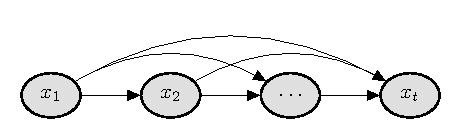
\includegraphics[width=0.9\textwidth]{cascade.pdf}
        \label{Markov:cascade}
    }%
    
    \subfigure[Second-order Markov model]{
        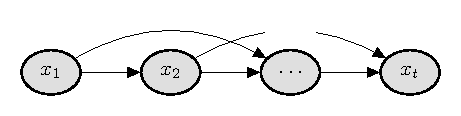
\includegraphics[width=0.9\textwidth]{second_order.pdf}
        \label{Markov:second_order}
    }%
    
    \subfigure[First-order Markov model]{
        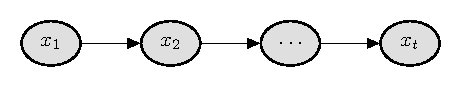
\includegraphics[width=0.9\textwidth]{first_order.pdf}
        %\caption{First-order Markov model}
        \label{Markov:first_order}
    }
    \caption{Graphical models for different time-series models}
    \label{Markov}
\end{figure}

The fundamental solution to this problem is the assumption of conditional independence. 
Intuitively, it corresponds to the removal of the edges in the cascade graph. 
One of the most well-known models for conditional independence assumption on time-series model is the Markov model. 
In which, $L$th-order Markov model assumes that given observation only depends on previous $L$ observations. 
Mathematically, assumption of the $L$th-order Markov model is as the following:

\begin{eqnarray}
    p\left(x_{t} \mid x_{1 : t-1}\right) & = & p\left(x_{t} \mid x_{t-L : t-1}\right)
\end{eqnarray}

Although $L$th-order Markov model is a simplified representation of the cascade graph, it still has relatively high complexity. 
On the other hand, the most straightforward representation of the Markov model is the $1$st-order Markov model, which assumes each observation in the sequence only depend on previous observation. 
It seems easy; however, it has a traceable posterior distribution, and therefore, it is an influential model which allows stronger modeling.
Mathematical interpretation of the first-order Markov model is as follows:

\begin{eqnarray}
    p\left(x_{t} \mid x_{1 : t-1}\right) & = & p\left(x_{t} \mid x_{t-1}\right)
\end{eqnarray}

Graphical models for cascaded graph, second($L$th)-order Markov model and first-order Markov model are shown in Figure~\ref{Markov:second_order} and Figure~\ref{Markov:first_order}, respectively. 
The complexity increases with the order of the network.

\section{Hidden Markov Model}
Up to the present, we examined the models which are directly built on observations.
However, such models are suffering from low representation power on data.
The reason for this is that observations are not always accurate and can deceive the model. 
Therefore, in the literature, a more general framework of time series models exists which uses latent, unobservable variable $s_t$, which generates observations.

From now on, instead of building models where observations depend on previous observations, we build models in which the observations depend on the hidden variable.
One of the most well-known models with this structure is the `state-space models' (SSM). 
In this model, each observation is assumed to be generated from a latent (or hidden) variable.
Therefore, Markov structure is formed on latent variables, $s_{1:\mathcal{T}}$, not on the observations, $x_{1:\mathcal{T}}$.
The observed variables are dependent on the hidden variables through an emission, $p\left(y_t \mid x_t\right)$\cite{barber2012bayesian}. 
Hidden Markov Model is the particular case of SSM in which hidden variables are only dependent on the previous hidden variable \cite{rabiner1989tutorial}.
Hence, state-transition dynamics are shown as $p\left(s_{t} \mid s_{t-1}\right)$.
In other words, Hidden Markov models are first order state-space models. Graphical model for HMMs is given in Figure~\ref{fig:hmm}. The joint probability distribution for this model is given below.
Initial state $s_1$ can be considered as dependent on initial hidden state $s_0$ and $p\left(s_1\right) = p\left(s_1 \mid s_0\right)$ so that one could get a simpler expression for joint probability.

\begin{eqnarray}
    p\left(s_{1 : \mathcal{T}}, x_{1 : \mathcal{T}}\right) & = & \left[\prod_{t=1}^{\mathcal{T}} p\left(x_{t} \mid s_{t}\right)\right]\left[\prod_{t=2}^{\mathcal{T}} p\left(s_{t} \mid s_{t-1}\right)\right]p\left(s_{1}\right) \\
    & = & \prod_{t=1}^{\mathcal{T}} p\left(x_{t} \mid s_{t}\right)p\left(s_{t} \mid s_{t-1}\right)\label{eq:hmm}
\end{eqnarray}

\begin{figure}
    \centering
    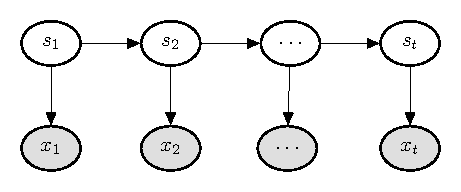
\includegraphics[width=0.9\textwidth]{figures/hmm.pdf}
    \caption{Graphical model for hidden Markov models or first-order state-space models}
    \label{fig:hmm}
\end{figure}

There are different naming for hidden Markov models because both discrete and continuous models share the same graphical model structure. 
For the convention, we use the term `state-space models'(SSM) as a generic name for latent state Markov models, `hidden Markov Model'(HMM) for the discrete latent state Markov models and `linear dynamical systems'(LDS) for continuous latent state Markov models.

The hidden variables in HMM are always discrete, while observations could be both discrete or continuous.
Therefore for a HMM, in the case of $S$ different states, the state transition distribution $p(s_{t}\mid s_{t-1})$ can be defined by an $S \times S$ transition matrix {\boldmath$\Psi$} and, $\Psi_{\hat{s}, \hat{s}^{\prime}}=p\left(s_{t}=\hat{s} \mid s_{t-1}=\hat{s}^{\prime}\right)$ denotes the probability of going from state $\hat{s}^{\prime}$ to state $\hat{s}$ at the time $t$. 
It is important to note that the transition matrix {\boldmath$\Psi$} is build from non-negative entries $\Psi_{\hat{s}, \hat{s}^{\prime}}$, and sum of entries in columns of transaction matrix is equal to 1, $\sum_{\hat{s}} \Psi_{\hat{s}, \hat{s}^{\prime}} = 1$
Similarly, in the case of $X$ discrete observations, emission distribution $p(x_t | s_t)$ can be defined  by $ X \times S$ emission matrix {\boldmath$\Omega$} and $\Omega_{\hat{x}, \hat{s}} = p\left(x_t = \hat{x} \mid s_t = \hat{s} \right)$. If the output is continuous then $s_t$ selects one of the potential $S$ output distributions $p(x_t \mid s_t)$.

\section{Inference in Hidden Markov Model}
\label{section:Inference-in-HMM}

Hidden Markov models have widespread applications with different purposes in many different domains, such as speech recognition, bioinformatics, and time series forecasting. Therefore, different outputs and statistics from the model may be requested.
One may try to infer the current latent state $s_t$ from the observations $x_{1:t}$. Mathematically, it can be shown as $p\left(s_t\mid x_{1:t}\right)$. 
This approach is named as {\it filtering} in the literature. 
On the other hand one can try to infer the past $p\left(s_{t-L}\mid x_{1:t}\right)$ or try to infer the future $p\left(s_{t+L}\mid x_{1:t}\right)$ with positive $L$, 
which are known as {\it smoothing} and {\it prediction} respectively. 
Finally one can try to identify the most likely hidden path $\arg\max_{s_{1 : \mathcal{T}}} p\left(s_{1 : \mathcal{T}} \mid x_{1 : \mathcal{T}}\right)$ which is known as {\it Viterbi path}. and can be calculated with {\it Viterbi algorithm}.
In the following parts, we will discover these methods.

\subsection{Filtering}
Filtering is the estimation of the current hidden state by using all observations so far, $p\left(s_t \mid x_{1:t}\right)$. 
To compute that, one can first find joint marginal $p\left(s_t,x_{1:t}\right)$ which is proportional to conditional marginal $p\left(s_t\mid x_{1:t}\right)$ and conditional marginal can be reached by the normalization.

\begin{eqnarray} 
p\left(s_{t}, x_{1 : t}\right) & = & \sum_{s_{t-1}} p\left(s_{t}, s_{t-1}, x_{1 : t-1}, x_{t}\right) \\ 
& = & \sum_{s_{t-1}} p\left(x_{t} \mid x_{1 : t-1}, s_{t}, s_{t-1}\right) p\left(s_{t}\mid x_{1 : t-1}, s_{t-1}\right) p\left(x_{1 : t-1}, s_{t-1}\right)\\ 
& = & \sum_{s_{t-1}} p\left(x_{t} \mid s_{t}\right) p\left(s_{t} \mid s_{t-1}\right) p\left(s_{t-1}, x_{1 : t-1}\right) \label{eq:filtering}
\end{eqnarray}

If we define $\alpha \left(s_t\right) = p\left(s_{t}, x_{1 : t}\right)$ and put that in the equation \ref{eq:filtering} we could get {\it $\alpha$-recursion} or {\it forward recursion};

\begin{eqnarray}
    \alpha\left(s_{t}\right) & = & \underbrace{p\left(x_{t} \mid s_{t}\right)}_{\text { corrector }} \underbrace{\sum_{s_{t-1}} p\left(s_{t} \mid s_{t-1}\right) \alpha\left(s_{t-1}\right)}_{\text { predictor }} \label{eq:filtering2}
\end{eqnarray}

where $\alpha \left(s_1\right) = p\left(x_{1}, s_{1}\right) = p\left(x_{1} \mid s_{1}\right)p\left(s_{1}\right)$. This recursive formula shows that filtered distribution $\alpha(.)$ is propagated through forward in each step and it acts like a `prior' distribution for the following time step. In other words, at each time step the previous posterior becomes the new prior \cite{barber2012bayesian}.

\subsection{Smoothing}

Smoothing is basically the estimation of the past from the given data.
Mathematically it can express as $p(s_t\mid x_{1:\mathcal{T}})$ where the $\mathcal{T}$ is usually the length of the sequence.
Similar to what have we done in the previous section, we calculate the joint marginal $p(s_t,x_{1:\mathcal{T}})$ instead of conditional marginal.
There are two main approaches to calculate smoothing: {\it Parallel Smoother} and {\it Sequential Smoother}.

\subsubsection{Parallel Smoother}

In this approach, the posterior distribution is rewritten in the form with contributions from the past and the future, taking advantage of {\it d-separation} in the equation \ref{eq:d-seperation}. 
It is the best-known smoothing method in the literature \cite{rabiner1989tutorial}.
Algebraically it can be shown as follows.

\begin{eqnarray}
    p\left(s_{t}, x_{1 : \mathcal{T}}\right) & = & p\left(s_{t}, x_{1 : t}, x_{t+1 : \mathcal{T}}\right) \\
    & = & p\left(s_{t}, x_{1 : t}\right)p \left(x_{t+1 : \mathcal{T}} \mid s_{t}, x_{1 : t}\right) \\
    & = & \underbrace{p\left(s_{t}, x_{1 : t}\right)}_{\text { past }} p \underbrace{\left(x_{t+1 : \mathcal{T}} \mid s_{t}\right)}_{\text { future }} \label{eq:d-seperation}\\
    & = & \alpha\left(s_t\right)\beta\left(s_t\right)
\end{eqnarray}

where $\beta(s_t)$ is called as {\it $\beta$-recursion} or {\it backward recursion}. 
Since $\alpha(.)$ and $\beta(.)$ recursions are independent of each other, and they may be run in parallel. 
So, we have to derive the $\beta$-recursion as in the equation \ref{eq:backward}. It is as follows:

\begin{eqnarray} 
p\left(x_{t+1:\mathcal{T}} \mid s_{t}\right) & = & \sum_{s_{t+1}} p\left(x_{t+1}, x_{t+2:\mathcal{T}}, s_{t+1} \mid s_{t}\right) \\ 
& = & \sum_{s_{t+1}} p\left(x_{t+1} \mid x_{t+2 : \mathcal{T}}, s_{t+1}, s_{t}\right) p\left(x_{t+2:\mathcal{T}}, s_{t+1}\mid s_{t}\right) \\
& = & \sum_{s_{t+1}} p\left(x_{t+1} \mid s_{t+1}\right) p\left(s_{t+1} \mid s_{t}\right) p\left(x_{t+2:\mathcal{T}} \mid s_{t+1} , s_{t}\right) \\
& = & \sum_{s_{t+1}} p\left(x_{t+1} \mid s_{t+1}\right) p\left(s_{t+1} \mid s_{t}\right) p\left(x_{t+2:\mathcal{T}} \mid s_{t+1}\right) \label{eq:backward} \\
\beta(s_t) & = & \sum_{s_{t+1}} p\left(x_{t+1} \mid s_{t+1}\right) p\left(s_{t+1} \mid s_{t}\right) \beta\left(s_{t + 1}\right)
\end{eqnarray}

This $\alpha - \beta$ recursion is known as {\it Forward-Backward} algorithm. Smoothed posterior can be obtained by the normalization of the result of the {\it Forward-Backward} algorithm.

\subsubsection{Sequential Smoother}

In this approach, the recursion is directly formed for smoothed posterior.
In the literature, it is known as {\it correction smoother}. This method also uses the power of the {\it d-separation} in a different manner. 
It makes future observations unnecessary by the conditioning on the latent present state \cite{rauch1965maximum}.

\begin{eqnarray}
    p\left(s_{t} \mid x_{1 : \mathcal{T}}\right) & = & \sum_{s_{t+1}} p\left(s_{t}, s_{t+1} \mid x_{1 : \mathcal{T}}\right) \\
    & = & \sum_{s_{t+1}}p\left(s_{t} \mid s_{t+1} , x_{1 : t}, x_{t+1:\mathcal{T}}\right)p\left(s_{t+1} \mid x_{1:\mathcal{T}}\right) \\
    & = & \sum_{s_{t+1}}p\left(s_{t} \mid s_{t+1} , x_{1 : t}\right)p\left(s_{t+1} \mid x_{1:\mathcal{T}}\right) \label{eq:sequential} \\
    \gamma(s_t) & = & \sum_{s_{t+1}} p\left(s_{t} \mid s_{t+1} , x_{1 : t}\right) \gamma(s_{t+1}) \label{eq:sequential-gamma}
\end{eqnarray}

%\vspace{20mm}
Equation~\ref{eq:sequential-gamma} could be obtained by setting $\gamma(s_t) = p(s_t \mid x_{1:\mathcal{T}})$.

In this smoother, the probability $p\left(s_{t} \mid s_{t+1} , x_{1 : t}\right) \propto p\left(s_{t+1}\mid s_t\right)p\left(s_t\mid x_{1:t}\right)$. 
So, it may directly be calculated from the filtered results. It is called {\it dynamic reversal} because it equals to change the directions in the latent space. 
This methods also named as {\it correction smoother} because it changed the filtered result. 
One could realize that sequential smoother is proportional to parallel smoother. 
%Mathematically it can be shown as;

\begin{eqnarray}
    \gamma \left(s_t\right) & \propto & \alpha \left(s_t\right) \beta \left(s_t\right)
\end{eqnarray}

\subsection{Prediction}

Prediction of the succeeding states and observations is another important topic in the latent space models. One can find the following sequence of length $L$ as follows:

\begin{eqnarray}
    p\left(x_{t+1:t+L} \mid x_{1 : t}\right) & = & \sum_{s_{t:t+L}} \left(\prod_{\tau=t+1}^{t+L} p\left(x_{\tau} \mid s_{\tau}\right) p\left(s_{\tau} \mid s_{\tau-1}\right)\right) p\left(s_{t} \mid x_{1 : t}\right) \label{eq:pred}
\end{eqnarray}

If the $L$-step ahead predictive distribution is more important than the predictive distribution of the $1$-step ahead, the sum is taken over future observations in the equation \ref{eq:pred}. So the new density is as follows:

\begin{eqnarray}
    p\left(x_{t+1:t+L} \mid x_{1 : t}\right) & = & \sum_{s_{t:t+L}} p\left(x_{t+L} \mid s_{t+L}\right)\left(\prod_{\tau=t+1}^{t+L} p\left(s_{\tau} \mid s_{\tau-1}\right)\right) p\left(s_{t} \mid x_{1 : t}\right)
\end{eqnarray}

\subsection{Viterbi Algortihm}

Finding the most likely sequence $s_{1:\mathcal{T}}$ of hidden states is significant problem\cite{viterbi1967error, forney1973viterbi}. The most likely sequence $s_{1:\mathcal{T}}$ for posterior $p\left(s_{1:\mathcal{T}}\mid x_{1:\mathcal{T}}\right)$ is the same with the most likely sequence for joint probability $p\left(s_{1:\mathcal{T}},x_{1:\mathcal{T}}\right)$. This joint probability is equivalent to equation \ref{eq:hmm}.

\begin{eqnarray}
    \underbrace{\max_{s_{1 : t}} p\left(s_{1 : t}, x_{1 : t}\right)}_{\phi \left(s_{t}\right)} & = & 
    \left(\max_{s_{t}}p\left(x_{t} \mid s_{t}\right) p\left(s_{t} \mid s_{t-1}\right) \right)
    \underbrace{\max _{s_{1 : t-1}} p\left(s_{1 : t-1}, x_{1 : t-1}\right)}_{\phi \left(s_{t-1}\right)}
\end{eqnarray}

In this recursion, the message is sent from the beginning to the end of the chain. 
From the set of observations $x_{1:\mathcal{T}}$, the Viterbi algorithm starts to find the most likely states $s_t$ beginning from the last.

\section{Learning in Probabilistic Models}

Learning is the estimation of the model parameters $\theta$ from the given data $\boldsymbol{x} \equiv x_{1:\mathcal{T}}$. 
Parameter estimation methods such as {\it maximum likelihood estimation} (MLE) and {\it maximum a posteriori} (MAP) are based on the idea of defining a probability distribution on data {$\boldsymbol{x}$} and tuning the parameters $\theta$ of the distribution such that likelihood of observed data is maximized under this particular probability distribution \cite{gauvain1994maximum}.
Maximum a Posteriori requires an additional prior distribution on parameters which is equivalent to regularization. Additionally, probability distributions are functions distributed between 0 and 1 and can take very small values. Therefore, for numerical stability, they are examined on a logarithmic scale, which is a monotonic function. So the general solution form is as follows;

\begin{itemize}
    \item {\it Maximum Likelihood Estimation}: $\arg \max _{\theta} \log p\left(\boldsymbol{x} \mid \theta\right)$
    \item {\it Maximum a Posteriori}: $\arg \max _{\theta} \log p\left(\theta \mid \boldsymbol{x}\right) \equiv \arg \max _{\theta} \left(\log p\left(\boldsymbol{x} \mid \theta\right)+\log p\left(\theta\right)\right)$
\end{itemize}

In latent space models, the hidden variables $\boldsymbol{s} \equiv s_{1:\mathcal{T}}$ should be marginalized out in order to calculate the likelihood of the data. In time series problem, since the hidden dimensions grows with time, it is usually impossible to track marginalization $\sum_{\boldsymbol{s}} p(\boldsymbol{x}, \boldsymbol{s} \mid \theta)$. Therefore it is impossible to calculate the likelihood of the data directly. Intractable likelihood of the HMM is as follows:

\begin{eqnarray}
    p\left(x_{1 : \mathcal{T}}\right)& = &\sum_{s_{\mathcal{T}}} p\left(s_{\mathcal{T}}, x_{1 : \mathcal{T}}\right) = \sum_{s_{\mathcal{T}}} \alpha\left(s_{\mathcal{T}}\right)
\end{eqnarray}

where $\alpha\left(s_{\mathcal{T}}\right)$ is shown in equation \ref{eq:filtering2}. 
So, the goal is the learning of the maximum likelihood parameters \cite{barber2011bayesian} which can be carried out by the following algorithms.
It is important to note that sum is exponential in the sequence length. Therefore, although the above formula appears straightforward, it is often impossible to calculate it directly.

\subsection{Expectation-Maximization Algorithm}

Maximizing the likelihood is an essential problem under missing data or latent variables \cite{dempster1977maximum}.
We mentioned that this is usually an intractable problem in time series models.
There is an iterative and convenient method in order to solve such problems, which is called {\it Expectation-Maximization} (EM) Algorithm.
The primary goal of the EM algorithm is to find a $\theta$ that maximizes the marginal likelihood $p(\boldsymbol{x}\mid \theta)$ or log marginal likelihood $\log p(\boldsymbol{x}\mid \theta)$. 
Since, the logarithm is a monotonic function, maximizing $\theta$ for these two likelihood is the same.
Usually, log marginal likelihood is preferred because it has numerical stability in calculations.
The main idea of the EM algorithm is to form an alternative objective function for which individual parameter updates can be achieved.
By doing so, the marginal likelihood will be replaced by a lower bound.
So, one can iteratively maximize this lower bound. 

To derive a lower bound on log marginal likelihood $\log p(\boldsymbol{x}\mid \theta)$, one could consider {\it Kullback-Leibler} (KL) divergence which measures the distance between probability distributions and is always non-negative\cite{kullback1951information}. 
In EM algorithm, one should define a `variational' distribution $q\left(\boldsymbol{s}\mid \boldsymbol{x}\right)$.
Then, the distance between `variational' distribution $q\left(\boldsymbol{s}\mid \boldsymbol{x}\right)$ and the parametric model $p\left(\boldsymbol{s}\mid \boldsymbol{x}, \theta \right)$ can be measured by KL divergence as follows:

\begin{align}
    \mathcal{D}_{\mathrm{KL}}\left( q\left(\boldsymbol{s}\mid \boldsymbol{x}\right) \| p\left(\boldsymbol{s}\mid \boldsymbol{x},\theta \right)\right) &=\mathbb{E}_{q\left(\boldsymbol{s}\mid\boldsymbol{x}\right)} \left[\log q\left(\boldsymbol{s}\mid\boldsymbol{x}\right) - \log p\left(\boldsymbol{s}\mid\boldsymbol{x}, \theta \right)\right] \\
    &=\mathbb{E}_{q\left(\boldsymbol{s}\mid\boldsymbol{x}\right)} \left[\log q\left(\boldsymbol{s}\mid\boldsymbol{x}\right) - \log p\left(\boldsymbol{s},\boldsymbol{x}\mid\theta \right)\right]
    + \log p\left(\boldsymbol{x}\mid\theta \right) \label{eq:KL}\\
    &\geq 0  \label{eq:KL0}
\end{align}

Equation \ref{eq:KL} is obtained from Bayes' rule $p\left(\boldsymbol{s}\mid\boldsymbol{x},\theta \right) = p\left(\boldsymbol{s}, \boldsymbol{x}\mid \theta \right) / p\left(\boldsymbol{x}\mid \theta \right)$ where $p\left(\boldsymbol{x}\mid \theta \right)$ does not depend on $\boldsymbol{s}$. So, lower bound on log marginal likelihood could be obtain by rearranging the inequality \ref{eq:KL} and \ref{eq:KL0}:

\begin{eqnarray}
    \log p\left(\boldsymbol{x} \mid \theta \right) &\geq& \underbrace{-\mathbb{E}_{q\left(\boldsymbol{s}\mid\boldsymbol{x}\right)} \left[\log  q \left(\boldsymbol{s}\mid\boldsymbol{x}\right) \right]}_{\text { Entropy }}
    +\underbrace{\mathbb{E}_{q\left(\boldsymbol{s}\mid\boldsymbol{x}\right)} \left[\log p\left(\boldsymbol{s},\boldsymbol{x}\mid\theta \right)\right]}_{\text { Energy }} \label{eq:ent-enr}
\end{eqnarray}

The right-hand side of the equation \ref{eq:ent-enr} is known as a lower bound for log-likelihood and represented as $\mathcal{L}(q, \theta)$ which is a function that depends on the choice of distribution $q$ and the model parameters $\theta$. Energy term is, on the other hand, known as `expected complete log-likelihood'\cite{barber2011bayesian}. 
One can show log-likelihood of the data as follows:
\begin{eqnarray}
    \log p\left(\boldsymbol{x} \mid \theta\right)&=&\mathcal{L}\left(q, \theta\right) + \mathcal{D}_{\mathrm{KL}}\left( q\left(\boldsymbol{s}\mid \boldsymbol{x}\right) \| p\left(\boldsymbol{s}\mid \boldsymbol{x},\theta \right)\right) \label{eq:loglik}
\end{eqnarray}

Therefore, by minimizing divergence in equation \ref{eq:loglik}, one can achieve to maximize the lower bound on the log-likelihood of the observations. The lower bound $\mathcal{L}$ depends both on model parameters $\theta$ and `variational distributions' $q$. 
The EM algorithm tries to find this lower bound iteratively by optimizing it w.r.t. $\theta$ and $q$, respectively.  This algorithm is built upon two steps which are;

\begin{itemize}
    \item {\it Expectation (E-step)}: Finds the variational distribution  $q\left(\boldsymbol{s}\mid \boldsymbol{x}\right)$ for fixed $\theta$
    \item {\it Maximization (M-step)}: Finds the model parameters $\theta$ for fixed $q\left(\boldsymbol{s}\mid\boldsymbol{x}\right)$
\end{itemize}

The algorithm starts with initial model parameters $\theta^{old}$. In the E-step, the variational distribution $q\left(\boldsymbol{s}\mid \boldsymbol{x}\right)$ is set to posterior distribution $p\left(\boldsymbol{s}\mid \boldsymbol{x}, \theta^{old}\right)$ and log-likelihood is calculated under $\theta^{old}$.
In the M-step, $\theta^{new}$ will be found which maximizes the log-likelihood. Since only the `energy' term of the lower bound in equation \ref{eq:ent-enr} depends on $\theta^{new}$, M-step corresponds to maximization of the energy.
By denoting `energy' as $Q\left(\theta , \theta^{o l d}\right)$, E and M steps could be shown as follows:

\begin{eqnarray}
    \text{E-step}:Q\left(\theta , \theta^{old} \right)&=&\mathbb{E}_{p\left(\boldsymbol{s} \mid \boldsymbol{x}, \theta^{old}\right)}\left[\log p\left(\boldsymbol{s}, \boldsymbol{x} \mid \theta\right)\right] \\ 
    \text{M-step}:\theta^{new}&=&\arg \max _{\theta} Q\left(\theta , \theta^{old}\right)
\end{eqnarray}

These steps are repeated until the convergence. E-step and M-step could also be considered as an inference step and learning step, respectively. In the E-step, posterior of the latent variables are inferred, and in the M-step, the new model parameters $\theta^{new}$ are learned.

\subsection{Baum-Welch Algorithm}

Baum-Welch algorithm is special case of the EM algorithm which is for learning model parameters of a hidden Markov model (HMM)\cite{tu2015derivation}. In the HMM, state transition matrix $\boldsymbol{\Psi}$, where $\Psi_{\hat{s}, \hat{s}^{\prime}}=p\left(s_{t}=\hat{s} \mid s_{t-1}=\hat{s}^{\prime}\right)$, emission matrix $\boldsymbol{\Omega}$, where $\Omega_{\hat{x}, \hat{s}} = p\left(x_t = \hat{x} \mid s_t = \hat{s} \right)$, and initial state parameter $\boldsymbol{\pi}$, where $\pi_{\hat{s}}=p\left(s_{t}=\hat{s}\right)$, could be learned from the given set of data $\boldsymbol{x}$ under the assumption that the number of hidden states S is known.
Therefore model parameters $\theta$ are parameterized by state transition $\boldsymbol{\Psi}$, emission probability $\boldsymbol{\Omega}$ and initial state $\boldsymbol{\pi}$, in such $\theta = \left(\boldsymbol{\pi}, \boldsymbol{\Psi}, \boldsymbol{\Omega}\right)$\cite{bishop2006pattern}.

The energy term of the HMM is obtained from the logarithm of the joint probability density of HMM in equation \ref{eq:hmm} under the assumption of the {\it independent and identically distributed} (i.i.d.) which is as follows:

\begin{eqnarray}
    Q\left(\theta , \theta^{old}\right) &=&\sum_{n=1}^{N} \mathbb{E}_{p\left(\boldsymbol{s}^{n} \mid \boldsymbol{x}^{n}, \theta^{o l d}\right)}\left[\log p\left(\boldsymbol{s}^{n}, \boldsymbol{x}^{n}\mid \theta\right)\right] \\
    &=&\sum_{n=1}^{N} \mathbb{E}_{p\left(s_{1}^{n} \mid \boldsymbol{x}^{n}, \boldsymbol{\pi}^{o l d}\right)}\left[\log p\left(s_{1}^{n}\right)\right] \nonumber\\
    & &+\sum_{n=1}^{N}\sum_{t=2}^{\mathcal{T}_{n}}\mathbb{E}_{p\left(s_{t}^{n}, s_{t-1}^{n} \mid \boldsymbol{x}^{n}, \boldsymbol{\Psi}^{old}\right)}\left[\log p\left(s_{t}^{n} \mid s_{t-1}^{n}\right)\right] \nonumber\\
    & &+\sum_{n=1}^{N}\sum_{t=1}^{\mathcal{T}_{n}}\mathbb{E}_{p\left(s_{t}^{n} \mid \boldsymbol{x}^{n}, \boldsymbol{\Omega}^{old}\right)}\left[\log p\left(x_{t}^{n} \mid s_{t}^{n}\right)\right] \label{eq:baum-welch}
\end{eqnarray}

One need to maximize energy term specified in equation \ref{eq:baum-welch}. We need to maximize this equation according to our three different parameters. This procedure corresponds to the M-step of the EM algorithm.

Optimizing Equation \ref{eq:baum-welch} with respect to $p\left(s_1\right)$ and forcing $p\left(s_1\right)$ to be a distribution one can get M-step of the initial parameters as follows:

\begin{eqnarray}
    \pi_{\hat{s}}^{n e w} \equiv p\left(s_{1}=\hat{s}\mid \theta^{old}\right)&=&\frac{1}{N} \sum_{n=1}^{N} p\left(s_{1}^{n}=\hat{s} \mid \boldsymbol{x}^{n}, \theta^{old}\right)
\end{eqnarray}

This is the average number of time where initial state $s_1$ is in state $\hat{s}$ w.r.t. $\boldsymbol{\pi}^{old}$. Similarly one should optimize equation \ref{eq:baum-welch} w.r.t. $p\left(s_t\mid s_{t-1}\right)$ to get M-step of the transition paramaters which is as follows:

\begin{eqnarray}
    \Psi_{\hat{s},\hat{s}^{\prime}}^{n e w} &\equiv& p\left(s_{t}=\hat{s} \mid s_{t-1}=\hat{s}^{\prime}, \theta^{old}\right) \\
    &\propto& \sum_{n=1}^{N} \sum_{t=2}^{\mathcal{T}_{n}} p\left(s_{t}^n=\hat{s}, s_{t-1}^n=\hat{s}^{\prime} \mid \boldsymbol{x}^{n}, \theta^{old}\right)
\end{eqnarray}

Which is equivalent to the average number of times that transition from latent state $\hat{s}^{\prime}$ to $\hat{s}$. By enforcing the rows of the $\boldsymbol{\Psi}$ to be a distribution, we get the following equation:

\begin{eqnarray}
    \Psi_{\hat{s},\hat{s}^{\prime}}^{n e w} &=&\frac{\sum_{n=1}^{N} \sum_{t=2}^{\mathcal{T}_{n}} p\left(s_{t}^n=\hat{s}, s_{t-1}^n=\hat{s}^{\prime} \mid \boldsymbol{x}^{n},\theta^{old}\right)} {\sum_{\hat{s}} \sum_{n=1}^{N} \sum_{t=2}^{\mathcal{T}_{n}} p\left(s_{t}^n=\hat{s}, s_{t-1}^n=\hat{s}^{\prime} \mid \boldsymbol{x}^{n}, \theta^{old}\right)}
\end{eqnarray}

Similar to the previous update equations, M-step for the emission parameters are obtained by the optimization of equation \ref{eq:baum-welch} w.r.t $p\left(x_t\mid s_{t}\right)$. Update equation is as follows:

\begin{eqnarray}
    \Omega_{\hat{x}, \hat{s}}^{new} &\equiv& p\left(x_{t}=\hat{x} \mid s_{t}=\hat{s}\right) \\
    &\propto& \sum_{n=1}^{N} \sum_{t=1}^{\mathcal{T}_{n}} p\left(s_{t}^n=\hat{s} \mid \boldsymbol{x}^{n}, \theta^{old}\right) \mathbb{I}\left[x_{t}^{n}=\hat{x}\right]
\end{eqnarray}

This is equivalent to the average probability of emission form latent state $\hat{s}$ to observation state $\hat{x}$. Similar to transition probability, to get stationary probability distribution on emission matrix $\boldsymbol{\Omega}$ we need to normalize this equation for emission probability as follows:

\begin{eqnarray}
    \Omega_{\hat{x}, \hat{s}}^{new} &=& \frac{\sum_{n=1}^{N} \sum_{t=1}^{\mathcal{T}_{n}} p\left(s_{t}^n=\hat{s} \mid \boldsymbol{x}^{n}, \theta^{old}\right) \mathbb{I}\left[x_{t}^{n}=\hat{x}\right]} {\sum_{n=1}^{N} \sum_{t=1}^{\mathcal{T}_{n}} p\left(s_{t}^n=\hat{s} \mid \boldsymbol{x}^{n}, \theta^{old}\right)}
\end{eqnarray}

In the E-step, three quantities $p\left(s_{1}^{n}=\hat{s} \mid \boldsymbol{x}^{n}, \theta^{old}\right)$, $p\left(s_{t}^n=\hat{s}, s_{t-1}^n=\hat{s}^{\prime} \mid \boldsymbol{x}^{n}, \theta^{old}\right)$ and $ p\left(s_{t}^n=\hat{s} \mid \boldsymbol{x}^{n}, \theta^{old}\right)$ which are used in M-step update equations, should be calculated. The derivations of this quantities are shown in the section \ref{section:Inference-in-HMM}.

\section{Deep Learning Sequence Models}

Up to the present, we examined statistical models and algorithms. 
However, deep learning techniques for making inferences in time series are also very successful. In this section, we will continue to more in-depth dive into such sequence models. We will be only interested in networks that produce an output at each time step.

A neural network (NN), in the case of artificial neurons, is called an artificial neural network (ANN). It resembles an interconnected group of neurons which mathematically correspond to non-linear activation functions. 
That is, neural networks are non-linear statistical data modeling or decision making tools which can be used to model complex relationships between inputs and outputs or to find patterns in data. 
Additionally, these structures are transformed into deep models with an increased number of layers.
We will use the name `traditional, fully connected feedforward network' for all similar models.
Such networks would have separate parameters for each input feature so they would need to learn all parameter space separately at each position in the sequence and assume that all inputs and outputs are independent of each other. 
To overcome this problem, we deep learning sequence models use the parameter sharing approach. 
Parameter sharing makes it possible to share features across different positions of the network.
By this modification, NN approaches would work in sequence prediction since it takes into account the previous inputs to predict the next output.

\subsection{Recurrent Neural Networks}

Recurrent Neural Networks (RNN) are the neural networks for processing sequence data, which contains cycles in the structure\cite{goodfellow2016deep}. 
In the literature, any NN with the cycles can be considered as an RNN. 
Such cycles allow detecting recurrences of patterns and networks share the same weights across several time-steps\cite{graves2012supervised}. 
This chain structure makes them powerful to analyze sequences and time series problems. 
The folded and unfolded computational graphs of the RNNs and LSTMS are shown in Figure~\ref{fig:rnn}.
These graphs represents the mapping between an input sequence $\boldsymbol{x}$ and 
corresponding output sequence $\boldsymbol{\hat{y}}$.
$\boldsymbol{\mathcal{L}}$ refers to loss and shown as $\mathcal{D}\left(\boldsymbol{y}\|\boldsymbol{\hat{y}}\right)$ while $\boldsymbol{\mathcal{W}}$'s correspond to the weight matrix of the network. $\boldsymbol{C}$ represents the neural network in the loop and called as `cell'.
These computational graphs inspire these networks with the loops where each loop in the network represents the influence of the previous value of each variable on the next value of the same variable.

\begin{figure}
    \centering
    \subfigure[RNN Cell]{
       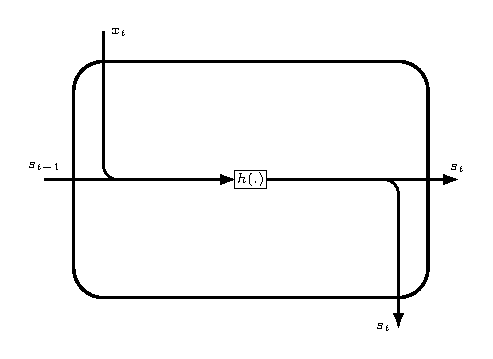
\includegraphics[width=0.48\textwidth]{figures/RNN_cell.pdf}
       \label{fig:rnn_cell}
    }%
  \hfill
  \subfigure[LSTM Cell]{
       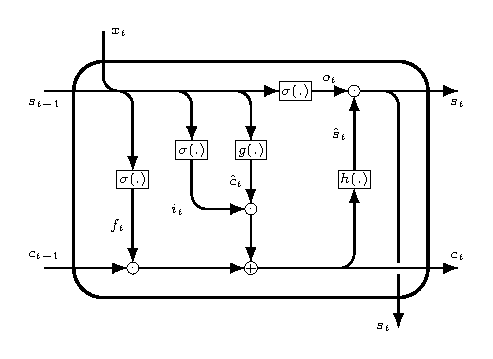
\includegraphics[width=0.48\textwidth]{figures/LSTM_cell.pdf}
       \label{fig:lstm_cell}
  }
    \caption{Cell structures of the RNN and LSTM, respectively}
    \label{fig:cells}
\end{figure}

The forward propagation of the RNN assumes that there is a non-linear activation function at the hidden units. Hidden state of the network is the result of this activation function. 
Outputs are the linear transformations of the hidden states. 
Graphically recurrent neural networks can be shown as Figure~\ref{fig:rnn} with the cell in Figure~\ref{fig:rnn_cell}.
Forward propagation begins with the $s_0$. Then for each time step following update equations will be applied:

\begin{eqnarray}
     s^{\prime}_{t} &=& \mathcal{W}_{ss}s_{t-1} + \mathcal{W}_{sx}x_t + b_s\\ 
     s_{t} &=& h \left(s^{\prime}_{t}\right) \\ 
     \hat{y}_{t} &=& \mathcal{W}_{ys}s_t + c_y
\end{eqnarray}

\begin{figure}
    \centering
    \subfigure{
       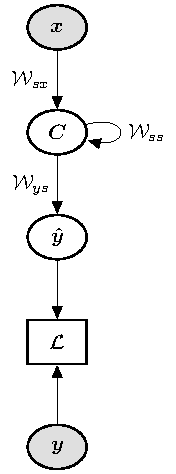
\includegraphics[width=0.231\textwidth]{figures/rnn_folded.pdf}
       \label{fig:rnn_folded}
    }%
  \hfill
  \subfigure{
       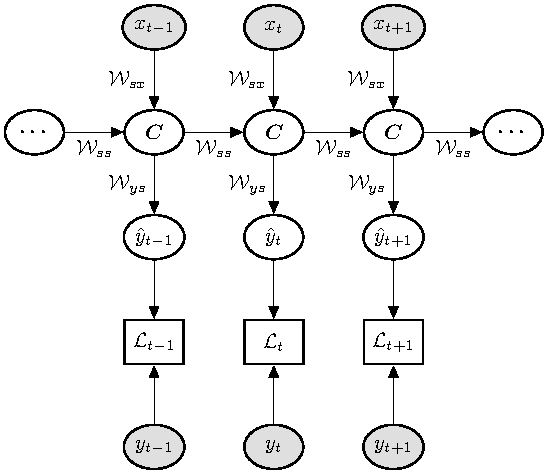
\includegraphics[width=0.7205\textwidth]{figures/rnn_unfolded.pdf}
       \label{fig:rnn_unfolded}
  }
    \caption{Folded and unfolded representation of the computational graphs, respectively}
    \label{fig:rnn}
\end{figure}

By the help of the chain structure and recurrence, these networks can learn sequences and patterns.
However, there are some disadvantages to RNNs. 
Since the gradients are transferred over time and pass through the activation function at each time step, the gradients tend to be decreasing exponentially and disappears after a few time steps. Therefore networks tend to forget the previous inputs after a few time steps and accordingly cannot handle the long-term dependencies.
This problem is usually called as the vanishing gradient \cite{hochreiter1998vanishing}.

\subsection{Long Short-Term Memory}

Learning long-term dependencies in dynamical systems is one of the main challenges in deep learning researches.
Long Short-Term Memory (LSTM) structure is designed for capturing long-term dependencies. 
They remember information for an extended period by default.
Therefore LSTMs have emerged as effective and scalable models for several learning problems related to sequential data \cite{hochreiter1997long}. They are a special kind of RNN that are good at learning long-term dependencies. 
Similar to all kind of RNNs, LSTMs have the form of a chain of repeating modules of neural networks \cite{olah2015understanding}. 

LSTM is a kind of gated RNN. The idea behind the gated RNNs is creating paths through time that have derivatives that neither vanish nor explode \cite{goodfellow2016deep}. Gated RNNs accomplish this idea by the gates that change connection weights at each time step. The central idea behind the LSTM architecture is a memory cell which can maintain its state over time, and non-linear gating units which regulate the information flow into and out of the cell \cite{greff2017lstm}.
The idea of introducing internal recurrence, in addition to the outer recurrence of the RNN, is to produce paths where the gradient can flow for long time-steps.
In standard RNN, repeating structure (cell) has a simple structure, an activation function. On the other hand, LSTM cell has four layers which interact with each other.
The combination of the Figure~\ref{fig:rnn} and Figure~\ref{fig:lstm_cell} could form graphical representation of the LSTMs.
Forward propagation and interactions in the single LSTM cell are derived step by step as following:

\begin{enumerate}
    \item It should be decided which information should be thrown away from the previous cell state. Decision is made by `forget gate' $f_t$. 
    It is derived as follows:
    \begin{eqnarray}
        f_t &=& \sigma\left(\mathcal{W}^{f}_{ss} s_{t-1} + \mathcal{W}_{sx}^{f} x_t + b^f \right)
    \end{eqnarray}
    \item It should be decided which new information coming from input $x_t$ will be stored in new cell state. In order to do this, first a proposal $\hat{c}_t$ should be made for the new cell state and then it should be decided how much of this proposal will be accepted. The decision maker for this process is the `input gate' $i_t$. These are derived as follows:
    \begin{eqnarray}
        \hat{c}_t &=& g\left(\mathcal{W}^{\hat{c}}_{ss} s_{t-1} + \mathcal{W}_{sx}^{\hat{c}} x_t + b^{\hat{c}} \right) \\
        i_t &=& \sigma\left(\mathcal{W}^{i}_{ss} s_{t-1} + \mathcal{W}_{sx}^{i} x_t + b^i \right)
    \end{eqnarray}
    \item The new step is the determination of the new cell state. For this purpose, the outputs obtained in the previous steps should be used. Derivation of the updated cell state is as follows:
    \begin{eqnarray}
        c_t &=& f_t \odot c_{t-1} + i_t \odot \hat{c}_t
    \end{eqnarray}
    \item The new hidden state $s_t$ is calculated after the calculation of the new cell status $c_t$. But this transformation is done in 3 steps. First, the cell state $c_t$ is passed through the activation function $h(.)$ as in RNN and unfiltered hidden state $\hat{s}_t$ is obtained. Then the obtained result is filtered by the `output gate' $o_t$ and the hidden state $s_t$ is obtained . The derivations as follows:
    \begin{eqnarray}
        \hat{s}_t &=& h\left(c_{t}\right) \\
        o_t &=& \sigma\left(\mathcal{W}^{o}_{ss} s_{t-1} + \mathcal{W}_{sx}^{o} x_t + b^o \right) \\
        s_t &=& o_t \odot \hat{s}_t
    \end{eqnarray}
    \item The predictions $\hat{y}_{t}$ of the network are obtained as follows. It is the linear transformation of the hidden state $s_t$ at time $t$, with the output weights of the network $\mathcal{W}_{ys}$, as in RNN.
    \begin{eqnarray}
        \hat{y}_{t} &=& \mathcal{W}_{ys}s_t + c_y
    \end{eqnarray}
\end{enumerate}

LSTMs are the improved version of the RNNs. It has a better capacity of holding past information to current state and known as state of the art sequence model \cite{greff2017lstm}.

\subsection{Learning in RNN and LSTM}

After forward propagation, the loss $\mathcal{L}$ between $y_t$ and $\hat{y}_t$ and gradients will be calculated. Computation of the gradients through an RNN and an LSTM is a straightforward problem\cite{goodfellow2016deep}. A particular version of the backpropagation algorithm, which is known as {\it Backpropagation Through Time} (BPTT), should be applied \cite{werbos1990backpropagation}. 
BPTT operates on an unfolded computational graph of RNN in time. The unfolded network contains $t$ inputs and outputs, but the network shares the same parameters over all networks. Then the backpropagation algorithm is used to find the gradient of the loss function concerning all the network parameters.

\chapter{MODELS AND ALGORITHMS FOR ANOMALY DETECTION}
\label{chapter:models-and-algorithms-for-anomaly-detection}
In chapter 1, we briefly mentioned the anomaly detection in time series problem and showed that several studies in the literature address different approaches for the problem. 
In chapter 2, we mentioned the models and inference algorithms that are necessary for the development of anomaly detection in time series applications. 
In this chapter, the development of anomaly detection algorithms will be examined. 
Anomaly detection models should be able to distinguish the anomalies arising from the outliers in the system and the anomalies resulting from the errors in the observations.
Besides, these models should be able to cope with missing observations to achieve more fruitful results, because such missing observations may disrupt the resulting anomaly score.
Another issue is the importance of the models that can detect anomalies online because the anomalies are often wanted to be detected as soon as possible, even before they happen.
The rest of this section contains details about the works we have done by paying attention to the above details.

\section{Gaussian Mixture Model for Anomaly Detection}

The problem of anomaly detection is more common in real data than in virtual data. 
Therefore, while modeling the system, it should be ensured that erroneous observations do not disturb the model. 
Therefore, we should be able to model these erroneous observations while developing our model.
In other words, we can say that systems feed on multiple sources where one of them produce erroneous observations.
If we can develop a model in this way, we can better detect system behavior and detect anomalies.
We can develop such a model with Gaussian mixtures.
Let assume; we have a one-dimensional observation. We assume that these observations come from 2 different distributions.
So, we define two distributions. The first one is for non-outlier observations, and it has Gaussian distribution with a mean and ideal amount of variance that is calculated during the expectation maximization process. The second distribution is for outlier observations and has $0$ mean and $\infty$ variance. Then, let us assume, there is another Bernoulli distributed parameter $r$ which decides either given observation is an outlier or not. 
Then, we evaluate the model for parameters of the first distribution during the process. So our generative model is as follows:

\begin{eqnarray}
    r_t &\sim& \mathcal{BE}(\pi) \\
    p\left(y \mid x,r,\mu,\sigma\right) &\sim &\mathcal{N}\left(\mu,\sigma^2\right)^{r=0} \mathcal{N}\left(0,\Sigma\right)^{r=1}
\end{eqnarray}

Here, $r = 1$ represents the outlier observations and $r = 0$ represents the non-outlier ones. 
This model is intended to find the possibility of  $\mu^{(n+1)}$ and $\sigma^{(n+1)}$ which are maximizing the expectation of $\langle \log p\left(y,r\mid x,\mu,\sigma\right)\rangle$ under the probability distribution $p\left(r\mid x,y,\mu^{(n)},\sigma^{(n)}\right)$. So, the derivation of this is as follows:

\begin{eqnarray}
    \mu^{(n+1)},\sigma^{(n+1)}&=&\arg\max_{\mu,\sigma}\mathbb{E}_{p\left(r\mid x,y,\mu^{(n)},\sigma^{(n)}\right)} \left[\log p\left(y,r\mid x,\mu,\sigma\right)\right] \label{eq:mu-sigma}
\end{eqnarray}

If we derive the probability distribution inside the expectation in equation \ref{eq:mu-sigma}, we got the following equations:

\begin{eqnarray}
    p\left(y,r\mid x,\mu,\sigma\right) &=& \prod_t p\left(y_t,r_t\mid x_t,\mu,\sigma\right) \\
    &=&\prod_t p\left(y_t\mid x_t,r_t,\mu,\sigma\right)p\left(r_t\right) \\
    &=&\prod_t \left(\frac{1-\pi_0}{\sqrt{\tau*\sigma^2}}\exp\left(\frac{-(\mu_t-y_t)^2}{2*\sigma_t^2}\right)\right)^{(1-r_t)} \\
    & &\times\left(\frac{\pi_0}{\sqrt{\tau*\Sigma}}\exp\left(\frac{-y_t^2}{2*\Sigma}\right)\right)^{(r_t)} \label{eq:pd}
\end{eqnarray}

After the calculation of $p\left(y,r\mid x,\mu,\sigma\right)$, one can directly calculate the outlier probability $r$ given all other parameters. To calculate $r$, there is a need for the sum of the probability in Equation \ref{eq:pd} over $r$.
The derivation is as follows:

\begin{eqnarray}
    p\left(r\mid x,y,\mu,\sigma\right) &=& \frac{p\left(r,y\mid x,\mu,\sigma\right)}{p\left(y\mid x,\mu,\sigma\right)} \\
    &=& \frac{p\left(r,y\mid x,\mu,\sigma\right)}{\Sigma_r p\left(r,y\mid x,\mu,\sigma \right)}
\end{eqnarray}

From now on, we derived the conditional distribution of outlier probability $r$, $p\left(r\mid x,y,\mu,\sigma\right)$ and opened the formula of $p\left(y,r\mid x,\mu,\sigma\right)$. Now let $\pi_t^{(n)}$ be the probability of $r=1$ given all other parameters. Then $\pi_t^{(n)}$ will become;

\begin{eqnarray}
    \pi_t^{(n)} &=& p\left(r_t=1\mid x_t, y_t, \mu^{(n)} ,\sigma^{(n)}\right) \\
    \pi_t^{(n)} &=& \frac{\frac{\pi_0}{\Sigma}\exp\left(\frac{-y_t^2}{2*\Sigma}\right)}{\frac{\pi_0}{\Sigma}\exp\left(\frac{-y_t^2}{2*\Sigma}\right) + \frac{1-\pi_0}{\sigma}\exp\left(\frac{-(\mu_t-y_t)^2}{2*\sigma^2}\right)}
\end{eqnarray}

Now, we should calculate the log likelihood in the equation \ref{eq:mu-sigma}. The objective is the maximization of the log-likelihood. 
The derivations for the calculation of the log-likelihood is as follows:

\begin{eqnarray}
    \mathbb{E}_{p\left(r\mid x,y,\mu^{(n)},\sigma^{(n)}\right)} \left[\log p\left(y,r\mid x,\mu,\sigma\right)\right] &=&\sum_t \mathbb{E}_{p\left(r\mid x,y,\mu^{(n)},\sigma^{(n)}\right)} \left[\log p\left(y_t,r_t\mid x,\mu,\sigma\right)\right] \nonumber\\
    &=&\sum_t\Bigg\langle r_t\left(\frac{-y_t^2}{2\Sigma^2}\right) \Bigg\rangle \nonumber \\
    &+&\sum_t\Bigg\langle(1-r_t)\left(\left(\frac{-(\mu_t-y_t)^2}{2\sigma_t^2}\right) -log\sigma_t\right)\Bigg\rangle \nonumber\\
    Q(\mu,\sigma)&\propto& \sum_t(1-\pi_t^{(n)})\left(\frac{(\mu_t-y_t)^2}{2\sigma_t^2} + log\sigma_t\right)
\end{eqnarray}

Now, we can iteratively calculate the $\mu^{(n+1)}$ and $\sigma^{(n+1)}$ values that maximize $Q(\mu,\sigma)$ such that;

\begin{eqnarray}
\mu^{(n+1)} &=& \arg\max_{\mu} Q(\mu,\sigma^{(n)}) \\
\sigma^{(n+1)} &=& \arg\max_{\sigma} Q(\mu^{(n)},\sigma)
\end{eqnarray}  

\begin{figure}
    \centering
    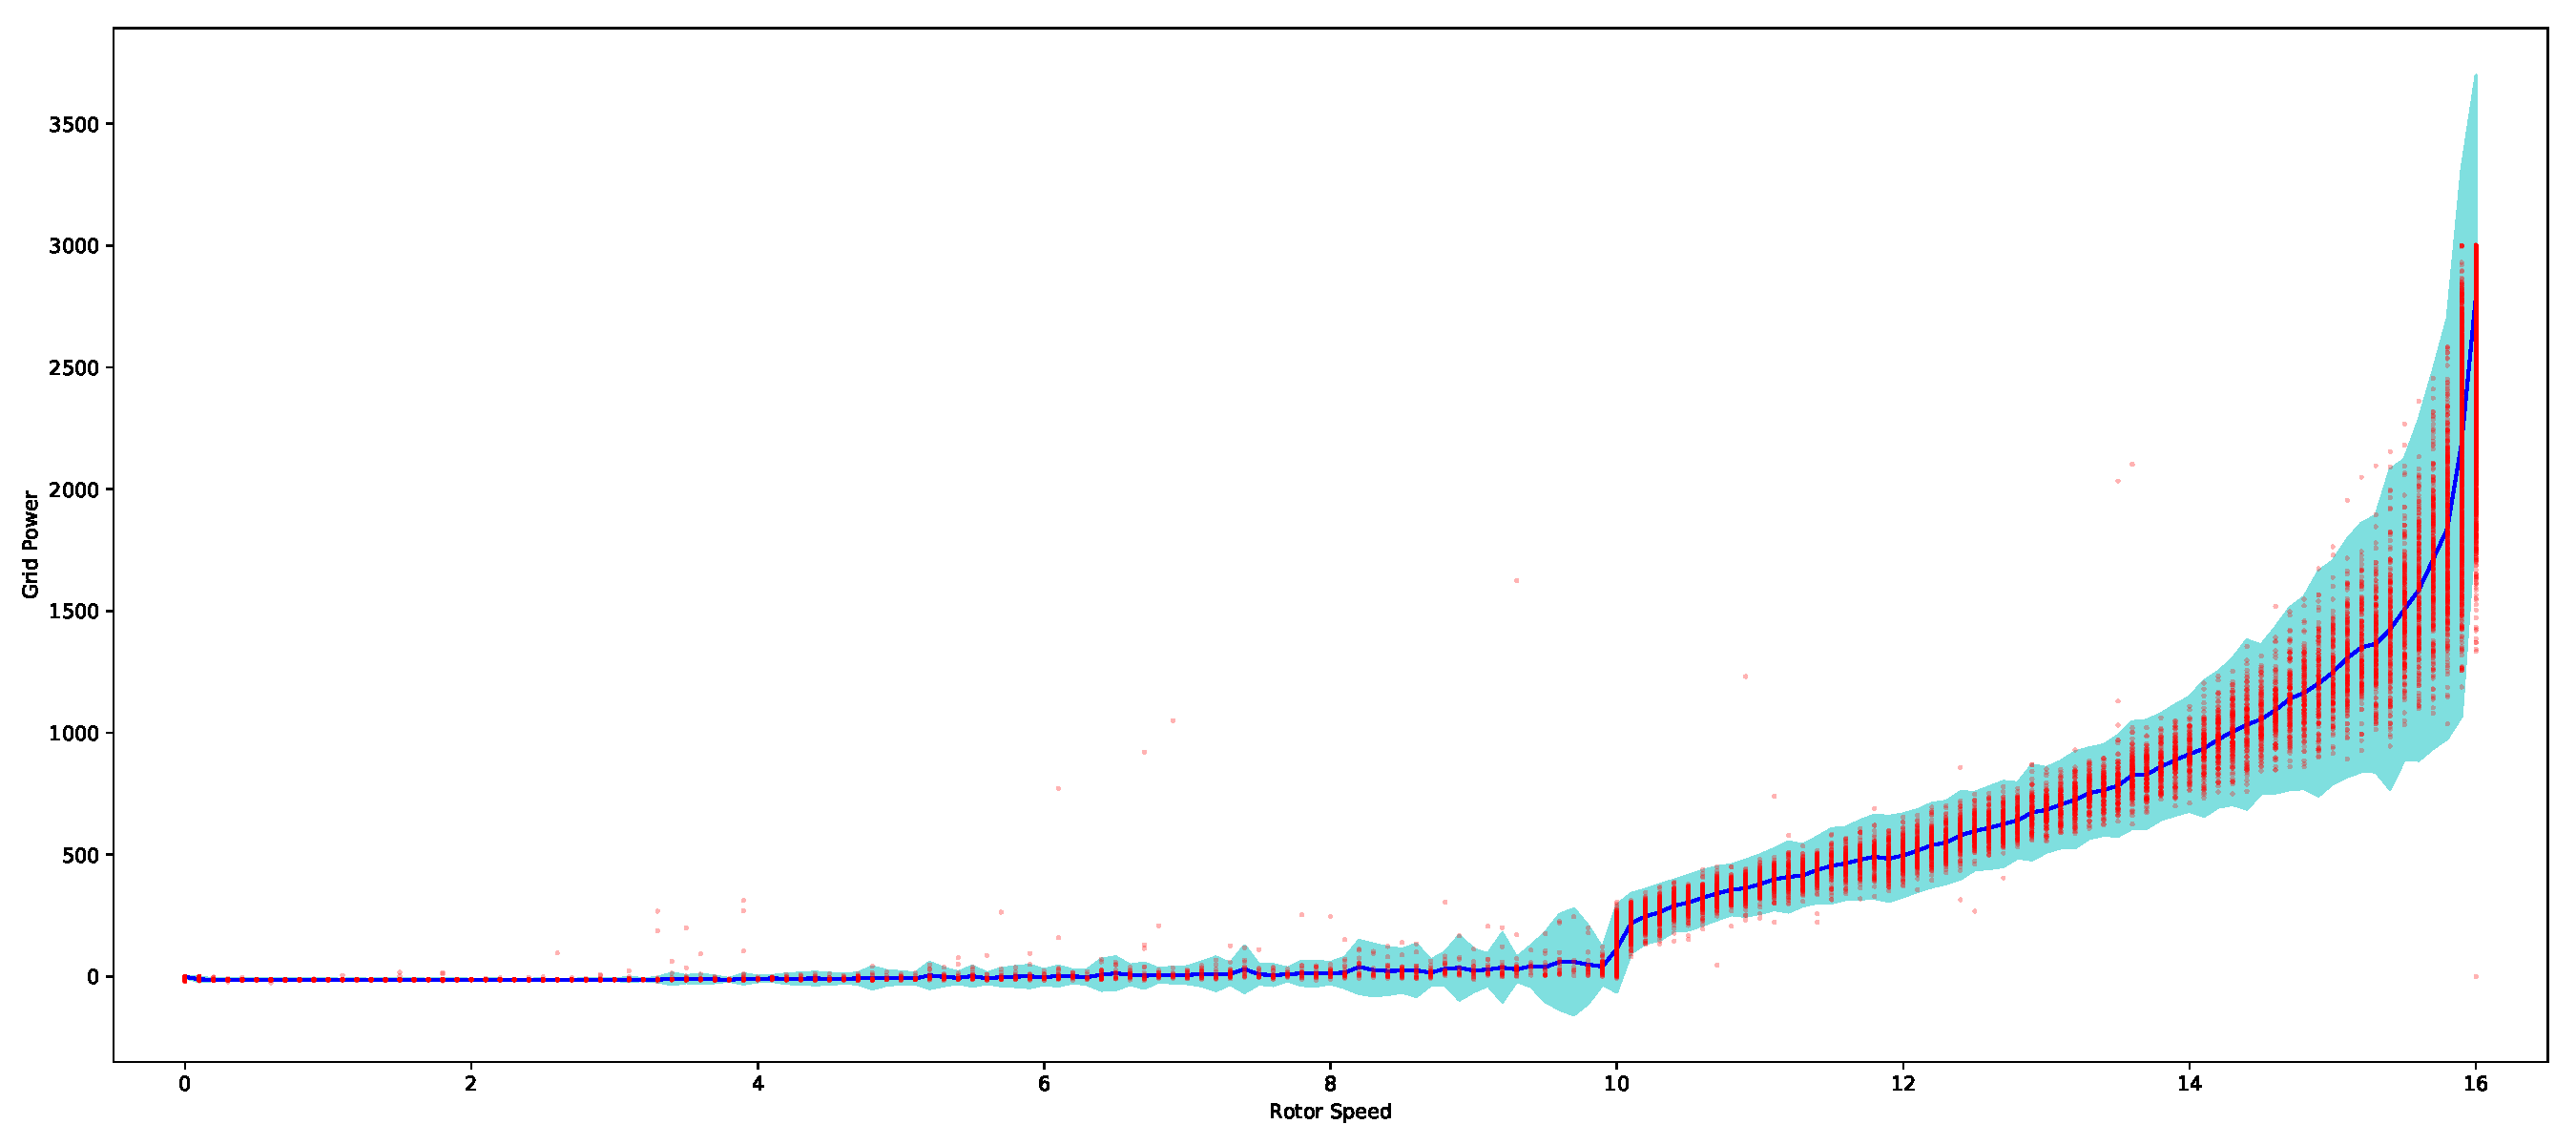
\includegraphics[width=0.85\textwidth]{figures/gmm-em.pdf}
    \caption{One dimensional Gaussian mixtures for the each value on the x-axis}
    \label{fig:gmm-em}
\end{figure}

In this model, we modeled the system without considering time series properties. Figure~\ref{fig:gmm-em} is showing the intuitive but straightforward example of the Gaussian mixtures. The model decides the outlier observations and then learns the system behaviors. The model learns the $r$ parameters during the test, and they will become the anomaly score of the system.

\section{Hidden Markov Model for Anomaly Detection}

The purpose of this section is to create a model that will learn the operation of a system as a time series and generate a warning against distortions and deterioration in this system. 
The model is also expected to catch anomalies in an unsupervised manner because the anomaly detection needs to be done online, and it is often not possible to find the data marked as an anomaly. 
Also, usually, there is not enough data available to model or validate the deterioration phase. 
For this reason, the behavior of the system in normal working conditions has been modeled. The model will generate a warning if the system works outside of the normal working conditions.

In this approach, the behavior of the system is modeled as a \textit{Hidden Markov Model}. 
Also, it is assumed that the system always selects a state from a \textit{discrete state space}, and according to this state, the system creates multi-dimensional observations. 
The state that the system chooses at any time depends only on the previous state. 
This state space corresponds intuitively with the phases that the system enters during operation (such as being closed or working on full power). 
However, one of the main difficulties of the problem is that the data set does not have an attribute, such as the phase of the system. 
Therefore, the state space should be found with the unsupervised learning algorithm. 
There are also some \textit{missing observations} and \textit{outliers} in the data set due to the sensors. 
These are other factors that must be accounted for in the Hidden Markov Model.

In the model, hidden variables of the system for the states at the $t$th time step is shown as $s_t$ and observations of the system at the $t$th time step is shown as $x_t$. 
Observations are usually multi-dimensional and expressed as a vector with a length of $\mathcal{P}+\mathcal{R}$ as $x_t = \begin{bmatrix} p_{t}^{1} & \cdots & p_{t}^{\mathcal{P}} & r_{t}^{1} & \cdots & r_{t}^{\mathcal{R}} \end{bmatrix}^T$. 
There are usually two kinds of the subgroup of observations which are observations that drives the system and observations that are driven by the systems and shown as $p^{1:\mathcal{P}}$ and $r^{1:\mathcal{R}}$, respectively. We will show $p^{1:\mathcal{P}}$ as $p$ and $r^{1:\mathcal{R}}$ as $r$ for the simplicity of the representation, unless otherwise required.

\subsection{Generative Model and Learning}

The discrete state space of the system consists of $S$ different states which indicate the typical operating phases, and there is $1$ additional state which indicates contradictory observations. In fact, with the slight modification of the observation model, instead of defining a separate state for the modeling of contradictory observations, it can be assumed that each observation is observed to be very noisy with a small likelihood. However, as far as we can tell from our analysis, outlier values are more likely to be seen in succession. For this reason, the state space of the model is defined in a way where there is an additional latent feature.

In our model the probability of transitions between states is shown in parameter $\boldsymbol{\Psi} \in \mathbb{R}^{(S+1) \times (S+1)}$. In other words, the transition probability from state $\hat{s}^{\prime}$ to state $\hat{s}$ is $\Psi_{\hat{s}, \hat{s}^{\prime}}$. Each situation has its own observation distribution. The observation distribution where the outliers are observed ($\hat{s}=0$) is a uniform distribution defined in the space of the observation. The observational distributions of the other states ($\hat{s}>0$) are multivariate Gaussian distributions with the variables $\mu_{\hat{s}}$ and $\Sigma_{\hat{s}}$:

\begin{eqnarray}
p(s_1) & = & \mathcal{U}\{0,S\} \\
p(s_{t} =\hat{s} \mid s_{t-1}=\hat{s}^{\prime}) & = & \Psi_{\hat{s} \hat{s}^{\prime}} \\
p(x_{t} \mid s_t = \hat{s}) & = &
\begin{cases}
c,& \hat{s} = 0 \\
\mathcal{N}(x_t;\mu_{\hat{s}},\Sigma_{\hat{s}}),& \hat{s} > 0 \\
\end{cases}
\end{eqnarray}

The next step is to calculate the variables $\Psi_{\hat{s} \hat{s}^{\prime}}$, $\mu_{\hat{s}}$ ve $\Sigma_{\hat{s}}$ from the data. Since this operation is expensive to perform over the whole dataset, random sequences with the length of $ \tau $ can be selected from the dataset. Let $x^{(i)}_{1:\tau}$ be the $i$th selected sequence and suppose that corresponding $s^{(i)}_{1:\tau}$ are known for this sequence. Then sufficient statistics for the variables can be calculated as follows:

{\small
    \begin{eqnarray}
    \Bigl< x_t x_t^T \Bigr>_{p(x_t \mid s_t = \hat{s})} &\approx& \mathcal{V}_{\hat{s}}^{(i)} = \frac{\sum_{t=1}^\tau [s^{(i)}_t = \hat{s}]  x_t x_t^T}{\sum_{t=1}^\tau [s^{(i)}_t = \hat{s}]} \label{eq:suff1}\\
    \Bigl< x_t \Bigr>_{p(x_t \mid s_t = \hat{s})} &\approx& m_{\hat{s}}^{(i)} = \frac{\sum_{t=1}^\tau [s^{(i)}_t = \hat{s}]  x_t }{\sum_{t=1}^\tau [s^{(i)}_t = \hat{s}]}\label{eq:suff2} \\
    C^{(i)}_{\hat{s}\hat{s}^{\prime}} & = & \sum_{t=2}^{\tau} [s^{(i)}_{t-1} = \hat{s}^{\prime}][s^{(i)}_{t} = \hat{s}] \label{eq:suff3}
    \end{eqnarray}
}

The average of sufficient statistics ($\mathcal{V}_{\hat{s}}^{(i)}$, $m_{\hat{s}}^{(i)}$, $C^{(i)}_{\hat{s}\hat{s}^{\prime}}$) of selected sequences can be used to estimate the final values of $\mathcal{V}_{\hat{s}}$, $m_{\hat{s}}$ ve $C_{\hat{s}\hat{s}^{\prime}}$. \textit{Moving averages} can be computed using a $\eta_i$ variable in the range $[0,1]$ to make this process less costly. Estimation of variables of distributions from the sufficient statistics are as follows:

\begin{eqnarray}
\Psi_{\hat{s}\hat{s}^{\prime}} & \approx & C_{\hat{s}\hat{s}^{\prime}}/\sum_k C_{k\hat{s}^{\prime}}  \\
\mu_{\hat{s}} & \approx & m_{\hat{s}}  \\
\Sigma_{\hat{s}} & \approx & \mathcal{V}_{\hat{s}} - m_{\hat{s}} m_{\hat{s}^{\prime}}^T
\end{eqnarray}

The states $s^{(i)}_{1:\tau}$ must be known for the calculations of equations in \ref{eq:suff1}, \ref{eq:suff2} ve \ref{eq:suff3}. If the variables $\Psi_{\hat{s}\hat{s}^{\prime}}$, $\mu_{\hat{s}}$ and $\Sigma_{\hat{s}}$ are known, $s^{(i)}_{1:\tau}$ can be estimated using the following recursive equation with the \textit{Viterbi algorithm}:

\begin{eqnarray}
    \underbrace{\max _{s_{1 : t}^{(i)}} p\left(s_{1 : t}^{(i)}, x_{1 : t}^{(i)}\right)}_{\phi \left(s_{t}^{(i)}\right)}=
    \left(\max _{s_{t}^{(i)}}p\left(x_{t}^{(i)} \mid s_{t}^{(i)}\right) p\left(s_{t}^{(i)} \mid s_{t-1}^{(i)}\right) \right)
    \underbrace{\max _{s_{1 : t-1}^{(i)}} p\left(s_{1 : t-1}^{(i)}, x_{1 : t-1}^{(i)}\right)}_{\phi \left(s_{t-1}^{(i)}\right)}
\end{eqnarray}

Therefore, the desired variables can be deduced by a recursive algorithm which first assumes the states constant and makes \textit{maximization} over the variables and then assumes the variables constant and makes \textit{maximization} over the states.

If there are \textit{missing data}, the only thing that will change is the distribution of observations. Fortunately, one of the advantageous properties of the Gaussian distribution and the uniform distribution is that the \textit{marginal probability} can be easily calculated. For example, in the case where observation $p_*$ is not observed, the distribution with Gaussian joint distribution will be transformed from the $\mu$ and $\Sigma$ into $(\mathcal{P}+\mathcal{R}-1)$ dimensional Gaussian distributions obtained by subtracting all the rows and orders for the observation $p_*$.

\subsection{Calculation of Predictive Distribution}

In the previous section, the process of learning the normal working pattern of the system is performed. After that, the observed behavior should be evaluated with the learned model. In our opinion, calculating the \textit{predictive distribution} to do this task is one of the most efficient ways. One of the important points is that instead of the predictive distribution $p(x_t \mid x_{1:t-1})$ of $x_t$, predictive distribution of the system driven parameters conditioned on the parameter which drives the system $p(r_t \mid p_t, x_{1:t-1})$ is more meaningful. Because the behavior of the system is how the system produces its output under given external conditions.
The predictive distributions of the system driven observations, which are conditional on system driver parameters, are in fact the ratio of the predictive distribution of all observations to the predictive distribution of the system driver observations:

\begin{eqnarray}
p\left(r_t \mid p_t, x_{1:t-1}\right)
& = &  \frac{p\left(x_{t} \mid x_{1:t-1}\right)}{ p\left(p_t \mid x_{1:t-1}\right)}
\end{eqnarray}

Additionally, the predictive distributions of all observations and the predictive distributions of the system driver observations could be calculated by following recursive equations:

\begin{eqnarray}
p\left(x_{t} \mid x_{1:t-1}\right) 
& = & \sum_{s_t} p\left(x_t,s_t \mid x_{1:t-1}\right) \\
& = & \sum_{s_t} p\left(x_t \mid s_t\right) p\left(s_t \mid x_{1:t-1}\right) \\
& = & \sum_{s_t} p\left(x_t \mid s_t\right) \sum_{s_{t-1}} p\left(s_t, s_{t-1} \mid x_{1:t-1}\right) \\
& = & \sum_{s_t} p\left(x_t \mid s_t\right) \sum_{s_{t-1}} p\left(s_t \mid s_{t-1}\right) p\left(s_{t-1} \mid x_{1:t-1}\right) \\
p\left(p_{t} \mid x_{1:t-1}\right) 
& = & \sum_{s_t} p\left(p_t \mid s_t\right) \sum_{s_{t-1}} p\left(s_t \mid s_{t-1}\right) p\left(s_{t-1} \mid x_{1:t-1}\right)
\end{eqnarray}

In order to find $ p \left(s_ {t-1} \mid x_ {1: t-1}\right) $ probabilities in these equations, it is sufficient to find and normalize \textit{forward probabilities}. The forward probabilities can also be found in the following recursive equation:

\begin{eqnarray}
\underbrace{p\left(s_t, x_{1:t}\right)}_{\alpha(s_t)} & = & p\left(x_t \mid s_{t}\right) \sum_{s_{t-1}} p\left(s_t \mid s_{t-1}\right) \underbrace{p\left(s_{t-1}, x_{1:t-1}\right)}_{\alpha\left(s_{t-1}\right)}
\end{eqnarray}

In order to generate anomaly prediction $\mathcal{E}_t$ from predictive distribution, the performance of the predictive distribution calculated by HMM is compared with the performance of the uniform distribution. If the uniform distribution is better than HMM, $\mathcal{E}_t$ will be higher. We foresee these cases as anomalies:

\begin{eqnarray}
\mathcal{E}_t & = & \frac{c}{c+p\left(r_{t} \mid p_t, x_{1:t-1}\right)}
\end{eqnarray}

\section{Deep Learning Sequence Models for Anomaly Detection}

In this section, deep learning models are developed for anomaly detection in time series. 
The developed models in this section are also expected to handle missing observations, and they are developed to find deterioration and anomalies in the system. Since usually there is no deterioration or anomaly label, these model should be an unsupervised model. Therefore, the model uses the system outputs $r$ as a label and trained under system inputs $p$ and system outputs $r$. 
In other words, the model learns the system, not anomalies.
The developed model will perform analysis on time series; therefore, RNNs and LSTMs, which are deep learning sequence models, are used. 
We will decide on the anomalies according to the conformity of the observations to the outputs of the model.

In this approach, we designed deep models that learn the relationship between the system driver parameters (input) and the system driven parameters (output), and the model also learns patterns of the system from the given input. 
Both inputs and outputs are multidimensional and expressed as a vector with the lenghts of $\mathcal{P}$ and $\mathcal{R}$ as $p_t = \begin{bmatrix} p_{t}^{1} & \cdots & p_{t}^{\mathcal{P}} \end{bmatrix}^T$ and $r_t = \begin{bmatrix} r_{t}^{1} & \cdots & r_{t}^{\mathcal{R}} \end{bmatrix}^T$, respectively. 
Therefore the developed models should generate system driven observations from the system driver observations, so it will act as a kind of generative model and learn to generate outputs regarding the system behavior \cite{malhotra2015long}.
Because deep learning sequence models can learn system dynamics in more detail, we prefer to look at the error of the outputs instead of defining an outlier state as in HMM.

\subsection{Forward Propagation in RNN}

The inputs and outputs of the system are defined. Now, in this step, the model is expected to learn the pattern between inputs and outputs. 
Since these networks are expensive to perform over whole dataset, random sequence with length of $\tau$ can be selected at each training epoch. Let $p_{1:\tau}^{(i)}$ be the $i$th selected input sequence and $r_{1:\tau}^{(i)}$ is the corresponding output sequence. The model will calculate the predicted output sequence $\hat{r}_{1:\tau}^{(i)}$.
Forward propagation of RNN for this model is as follows:

\begin{eqnarray}
     s^{\prime}_{t} &=& \mathcal{W}_{ss}s_{t-1} + \mathcal{W}_{sp}p^{(i)}_t + b_s\\ 
     s_{t} &=& h \left(s^{\prime}_{t}\right) \\ 
     \hat{r}^{(i)}_{t} &=& \mathcal{W}_{rs}s_t + c_y \label{eq:rnn-result}
\end{eqnarray}

Where $b_s$ corresponds to bias terms in the hidden layer of the NN and $c_y$ corresponds to bias term in the output layer. $\mathcal{W}$s are the model weights that are learned through training. This forward propagation is calculated from $1:\tau$ for the $i$th subsequence at each epoch. There will be $\mathcal{T}/\tau$ subsequence at each training step. $\mathcal{T}$ corresponds to the number of total data instance.

\subsection{Forward Propagation in LSTM}

In a similar way with the RNN, random sequence with length of $\tau$ can be selected at each training epoch. Let $p_{1:\tau}^{(i)}$ be the $i$th selected input sequence and $r_{1:\tau}^{(i)}$ is the corresponding output sequence. The model will calculate the predicted output sequence $\hat{r}_{1:\tau}^{(i)}$, as in RNN.
The forward propagation of LSTM for such a model is as follows:

\begin{eqnarray}
    f_t & = & \sigma\left(\mathcal{W}^{f}_{ss} s_{t-1} + \mathcal{W}_{sp}^{f} p^{(i)}_t + b^f \right) \\
    \hat{c}_t & = & g\left(\mathcal{W}^{c}_{ss} s_{t-1} + \mathcal{W}_{sp}^{c} p^{(i)}_t + b^c \right) \\
    i_t & = & \sigma\left(\mathcal{W}^{i}_{ss} s_{t-1} + \mathcal{W}_{sp}^{i} p^{(i)}_t + b^i \right) \\
    c_t & = & f_t \odot c_{t-1} + i_t \odot \hat{c}_t \\
    \hat{s}_t & = & h\left(c_{t}\right) \\
    o_t & = & \sigma\left(\mathcal{W}^{o}_{ss} s_{t-1} + \mathcal{W}_{sp}^{o} p^{(i)}_t + b^o \right) \\
    s_t & = & o_t \odot \hat{s}_t \\
    \hat{r}^{(i)}_{t} & = & \mathcal{W}_{rs}s_t + c_y \label{eq:lstm-result}
\end{eqnarray}

Where $b$s correspond to the bias term in the gates and hidden layers, and $c_y$ is the bias at the output layer. $f_t, i_t$ and $o_t$ corresponds to forget gate, input gate, and output gate, respectively. $\hat{c}$ is the proposed cell state, while $c_t$ is the cell state of the network. In a similar manner, $\hat{s}_t$ is the proposed hidden state for the network, while $s_t$ is the filtered and resulted in the hidden state of the network. 

\subsection{Learning}

After the calculation of forward propagation and generation of the $\hat{r}^{(i)}_{1:\tau}$, the loss will be calculated. So, the objective is the minimization of the loss concerning {\boldmath$\mathcal{W}$} which is as follows:

\begin{eqnarray}
    \arg\min_{\boldsymbol{\mathcal{W}}} \mathcal{L} \left(r_{1:\tau}^{(i)} \| \hat{r}_{1:\tau}^{(i)}\right)
\end{eqnarray}

The loss will be calculated and then the weights, $\boldsymbol{\mathcal{W}}$, are updated with the time series specific gradient descent algorithm which is backpropagation through time (BPTT) at each time-step \cite{werbos1990backpropagation}. The forward propagation and the weight update procedure with BPTT algorithm will continue with the new sub-sequences $i^\prime$ at each epoch until the convergence. Thus, the model parameters, $\boldsymbol{\mathcal{W}}$, are learned. As a result of this procedure, the model is able to reproduce system outputs.

\subsection{Prediction and Anomaly Score}

We developed models which learn the system to be analyzed. 
The next step is to find anomalies.
After the training phase, let us assume that there is a sequence, with a length $\mathcal{T}$, and we represent it as $p_{1:\mathcal{T}}$. 
Then the model will calculate the predicted outputs $\hat{r}_{1:\mathcal{T}}$ with the learned weights and bias terms as in the equations \ref{eq:lstm-result} and \ref{eq:rnn-result}.
Then, to detect the anomalies, the loss $\mathcal{L}$ between the observed data $r_{1:\mathcal{T}}$ and model predictions $\hat{r}_{1:\mathcal{T}}$ should be calculated separately for each time step.

\begin{eqnarray}
    \mathcal{E}_t &=& \mathcal{L} \left(r_t \| \hat{r}_t\right)
\end{eqnarray}

We have linear units at the output layer; therefore, our predictions are the result of that linear units.
So, we need to select appropriate loss function. 
{\it Root mean square error} (RMSE), {\it mean square error} (MSE) and {\it mean absolute error} (MAE) are the most appropriate loss functions.
However, since system outputs are multi-dimensional and some of the sensors return numerically large values and dominate the error, such loss functions, especially MSE and RMSE, have drawbacks.
One way to handle this drawback is to use another distance metric, which measures the percentage error. This metric is called as a {\it mean absolute percentage error} (MAPE). However, it brings out other problems such as high error rate at the points where observations are too small.
Therefore, we use another solution.
We normalize all the inputs and outputs and model calculates the results and errors on the normalized data. When doing reconstruction, we unnormalize it. When it comes to producing an anomaly score, we are applying the following steps:

\begin{enumerate}
    \item Calculate the error of each observation and create an unnormalized anomaly score from the error for each observation.
    \item Calculate the average loss of the fake observations which are uniformly selected within the range of the space of the feature space.
    \item Compare unnormalized error with the uniformly selected samples error and create normalized anomaly score.
\end{enumerate}

We compare different loss functions; however, these are not the most appropriate loss functions for our study, except for L1 loss. 
The model we developed performs unsupervised learning. Therefore, our model should not be affected by anomalous observations in the training data while learning the system. 
So, we need a loss function that will not be influenced by the anomalies.
This demand is a severe problem in the robust statistics literature \cite{black1996unification}, and we use the {\it Tukey's biweight} loss function as a robust optimization method for a deep regression \cite{belagiannis2015robust}. 
Detailed analysis of the MSE loss, L1 loss, and Tukey's biweight loss could be found in Appendix \ref{chapter:comparison-of-the-loss-functions}.

Let $c$ represents the average loss of the uniformly selected random samples, and let $\mathcal{E}^{\prime}_t$ shows the unnormalized error for the $t$th observation. Then we can obtain normalized anomaly score with the following equation:

\begin{eqnarray}
\mathcal{E}_t & = & \frac{\mathcal{E}^{\prime}_t}{c+\mathcal{E}^{\prime}_t}
\end{eqnarray}

If there is a higher probability of error for the specified time step, then corresponding observation will be marked as an anomaly. For the detection of collective anomaly \cite{bontemps2016collective}, moving averages of the resulting errors can be computed using a $\eta$ variable in the range $[0,1]$, which is as follows:

\begin{eqnarray}
    \hat{\mathcal{E}}_t &=& \hat{\mathcal{E}}_{t-1} \times \eta + \mathcal{E}_t \times \left(1 - \eta\right)  
\end{eqnarray}

In this section, we developed two similar models which use RNN and LSTM, respectively. It is expected that LSTM should give more precise results if the system has long-term dependencies while RNN should give more accurate results if the system has only short-term dependencies.

%\include{experiments_results}
\chapter{EXPERIMENTS AND RESULTS}
\label{chapter:experiments-and-results}
In this chapter, we present applications of the anomaly detection models described in Chapter \ref{chapter:models-and-algorithms-for-anomaly-detection}.
%We start our experiments by applying probabilistic models.
In the beginning, we apply GMM, which does not take into account the sequential feature of the data, and then we implement the HMM, which is a probabilistic sequence model.
Then, we expand our work with the application of deep learning sequence models. 
We perform experiments and compare the results with models constructed on RNN and LSTM, respectively.

In the experiments, we will use the Borusan wind turbine dataset.
%and NASA Aircraft Engine datasets \cite{saxena2008damage, bao2018remaining}.

\section{Wind Turbine Dataset}

%We used Borusan Vestas V90-3MW wind turbines dataset as the first application of anomaly detection problem.
Borusan Vestas V90-3MW wind turbines dataset was created from 20 different wind turbines which are identical.
For each wind turbine, there are observations collected at 25737 different consecutive time-steps.
Each observation is the collection of wind speed, rotor speed, and generated power values.
This data set was created with data collected at 10-minute intervals from February to July.
There are only two reported anomalies in the data set. 
However, it is known that there are unreported and undetected anomalies.
Additionally, this dataset contains some Null and incorrect sensory information because of the faulty sensor measurements.
These errors occur randomly and do not continue.
Therefore, we know that there is no accurate data in the data set and that there are errors and missing data in the observations. The visualization of the wind, rotor, and power data could be found in Figure \ref{fig:data}.

\begin{figure}
\centering
    \subfigure[Wind speed graph as a time-series]{
        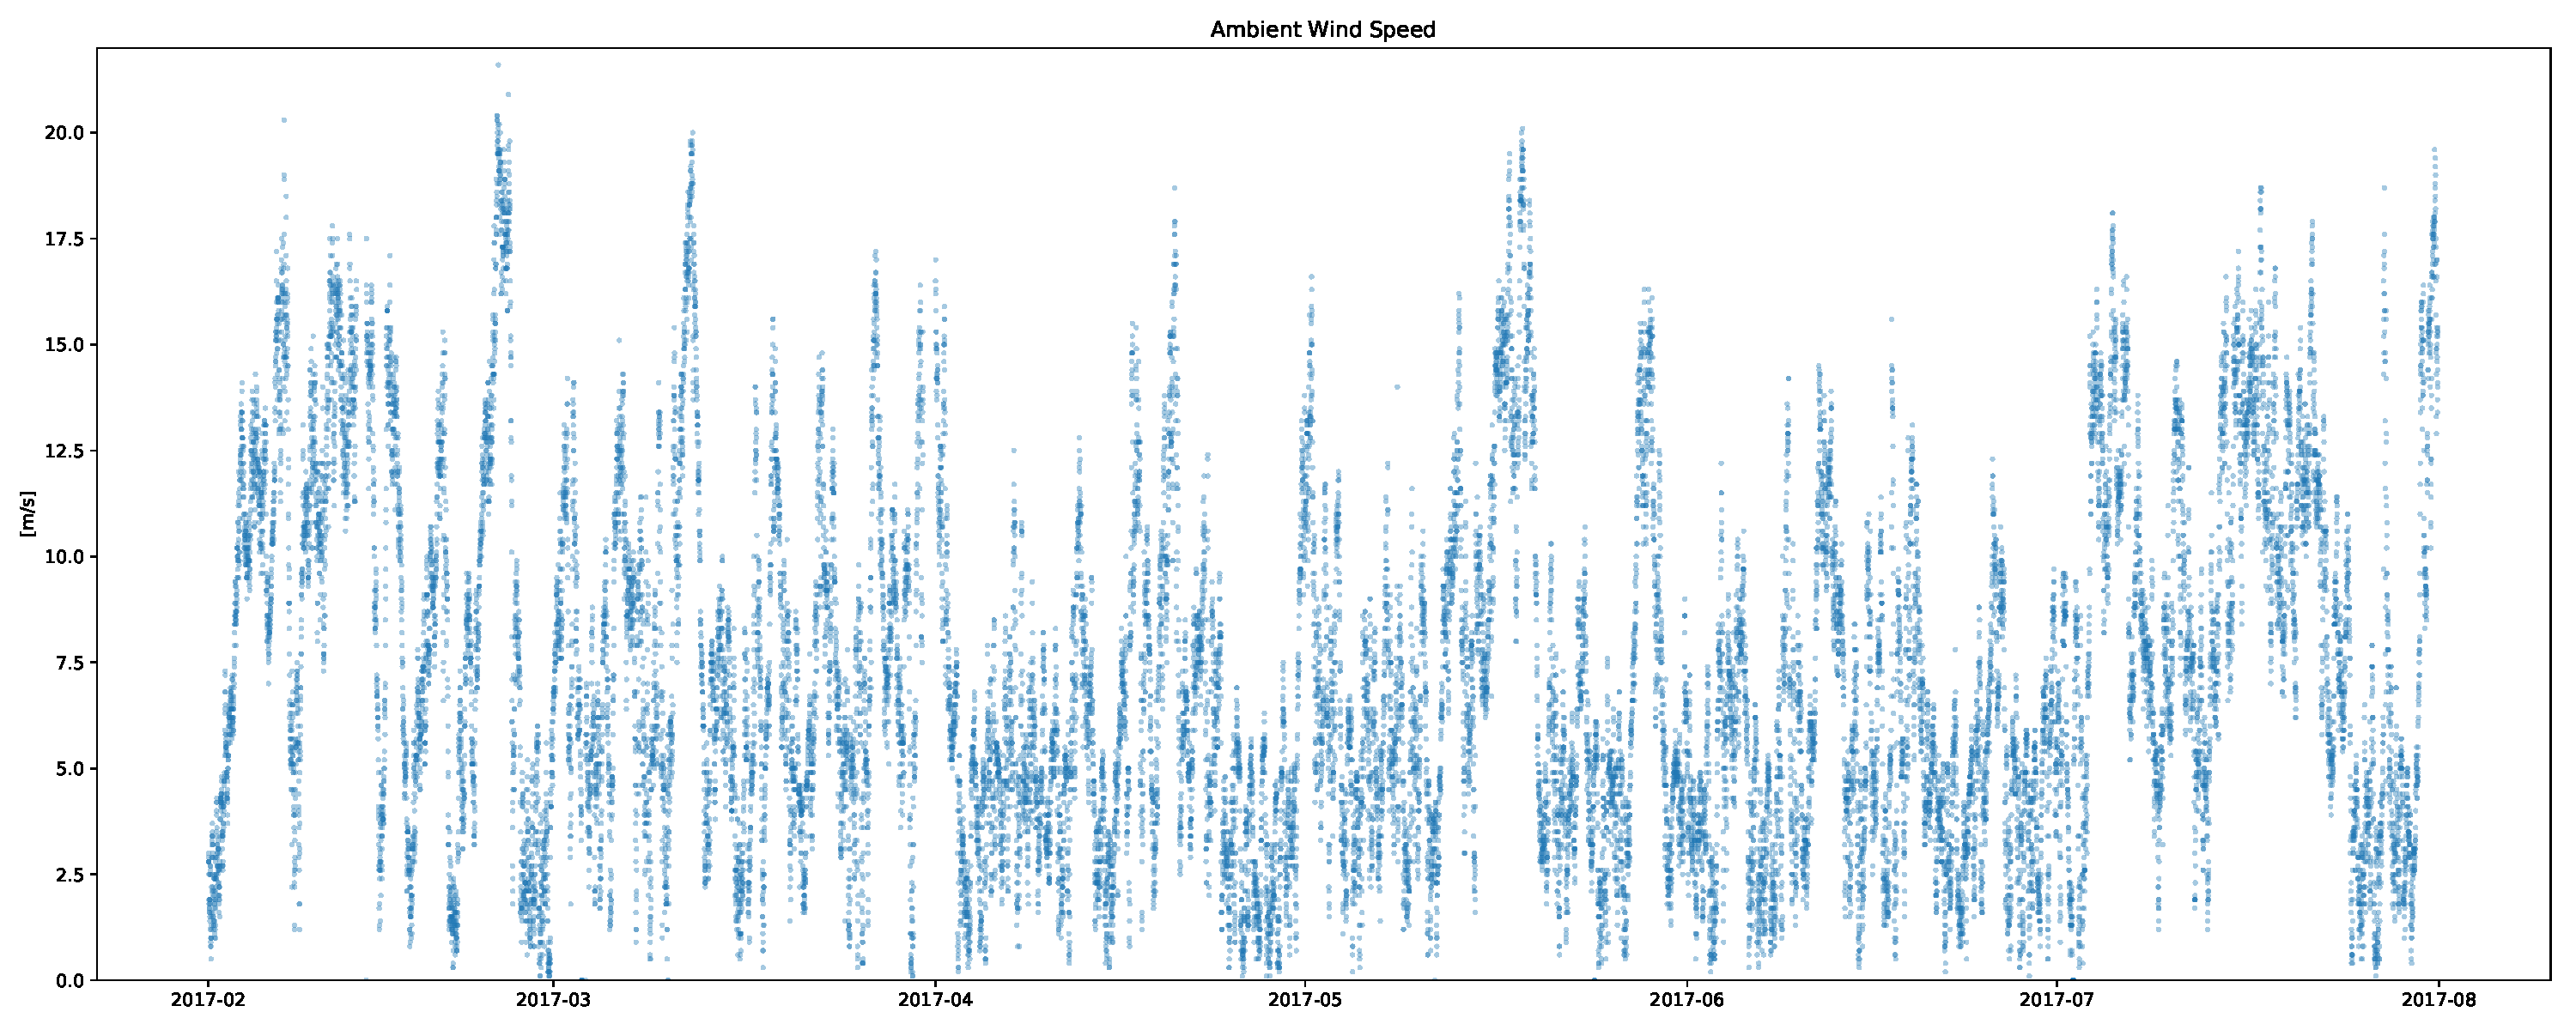
\includegraphics[width=0.9\textwidth]{wind.pdf}
        \label{fig:wind}
    }%
    
    \subfigure[Rotor speed graph as a time-series]{
        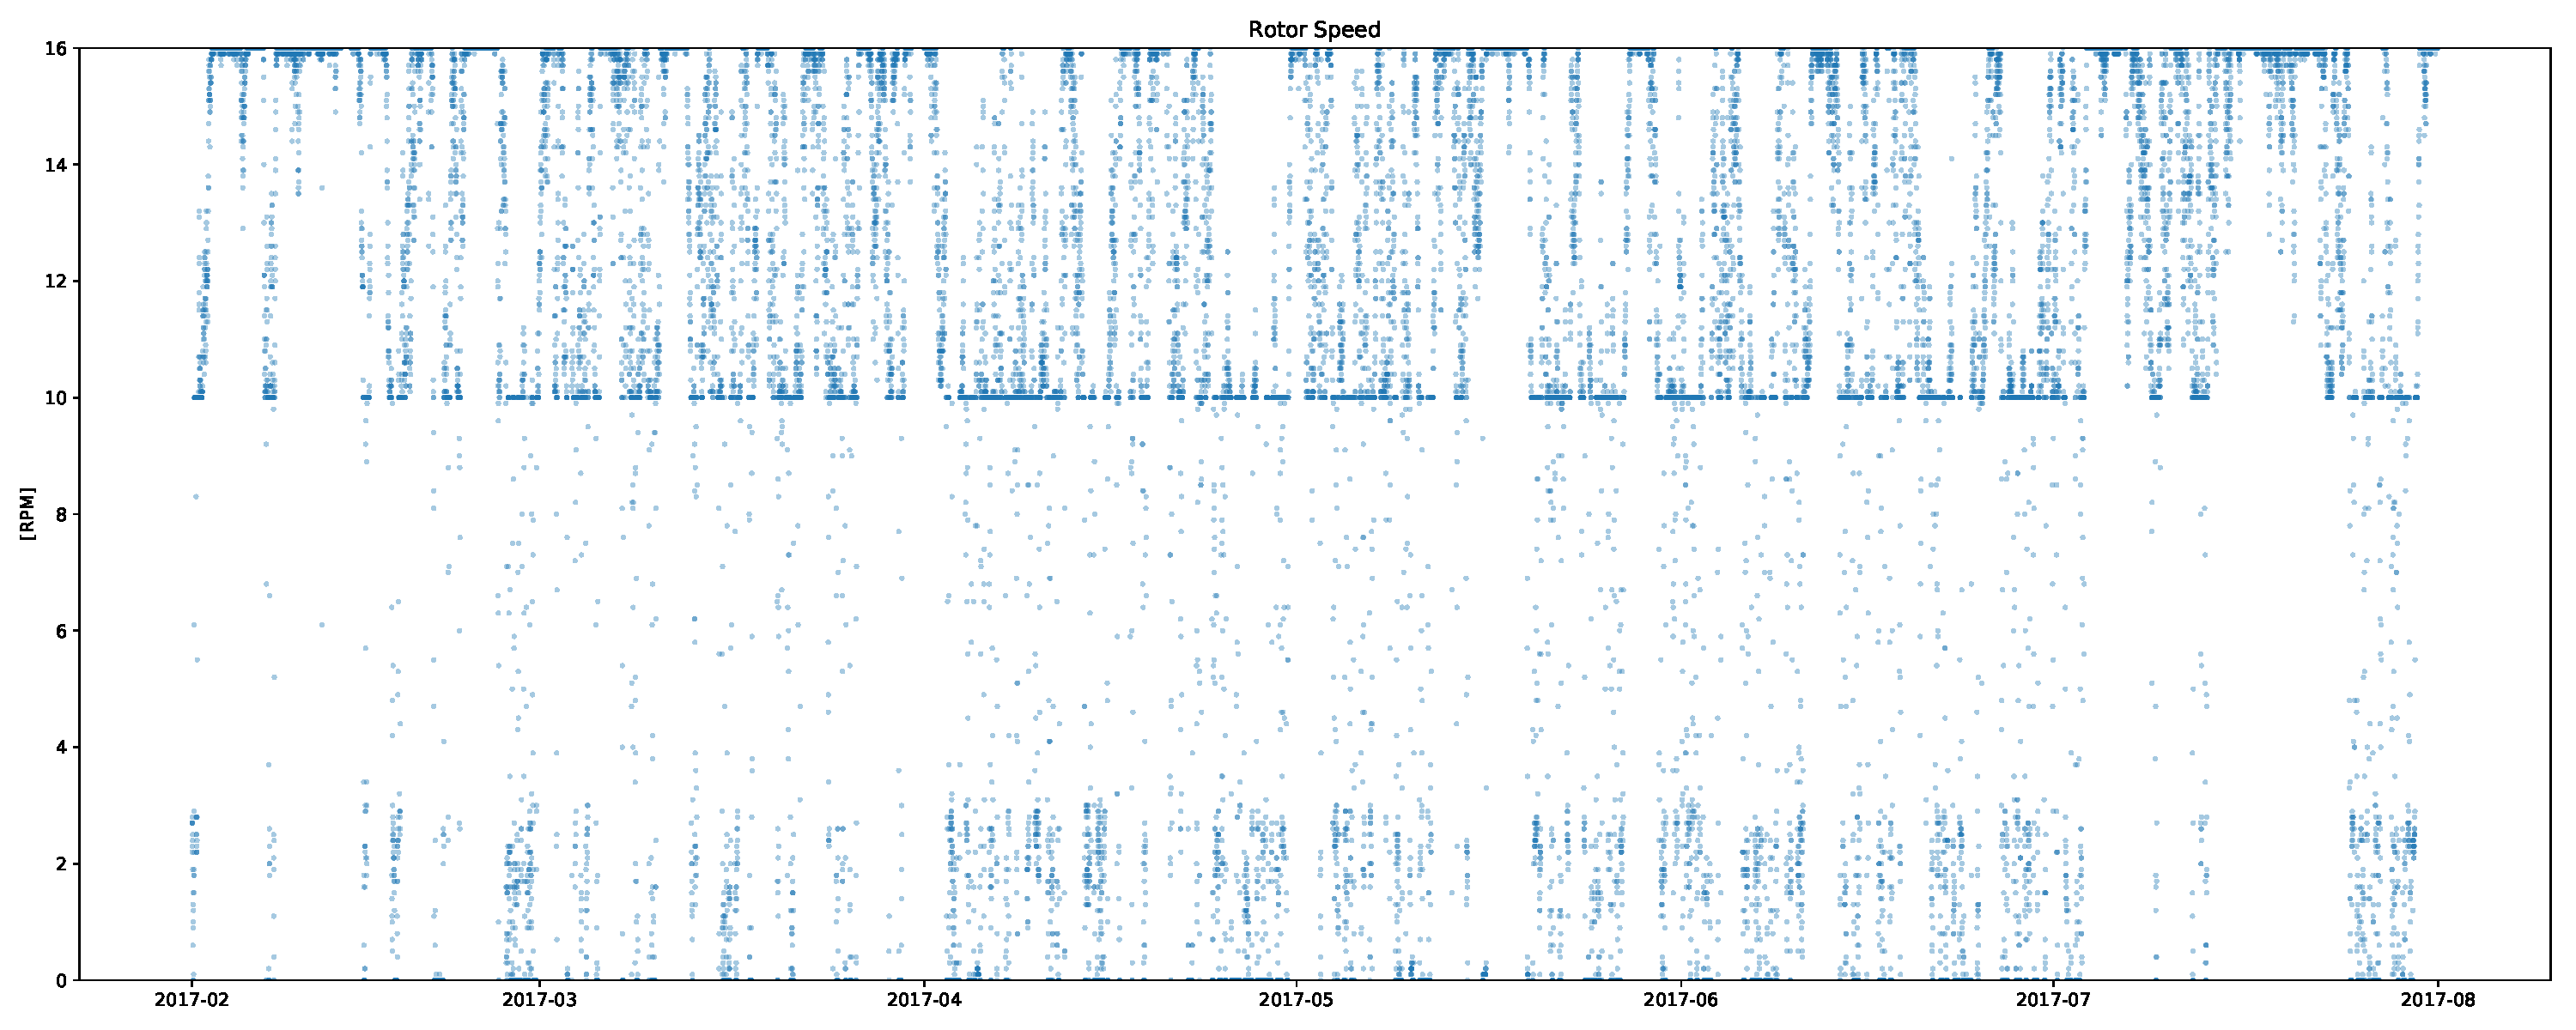
\includegraphics[width=0.9\textwidth]{rotor.pdf}
        \label{fig:rotor}
    }%
    
    \subfigure[Generated grid power graph as a time series]{
        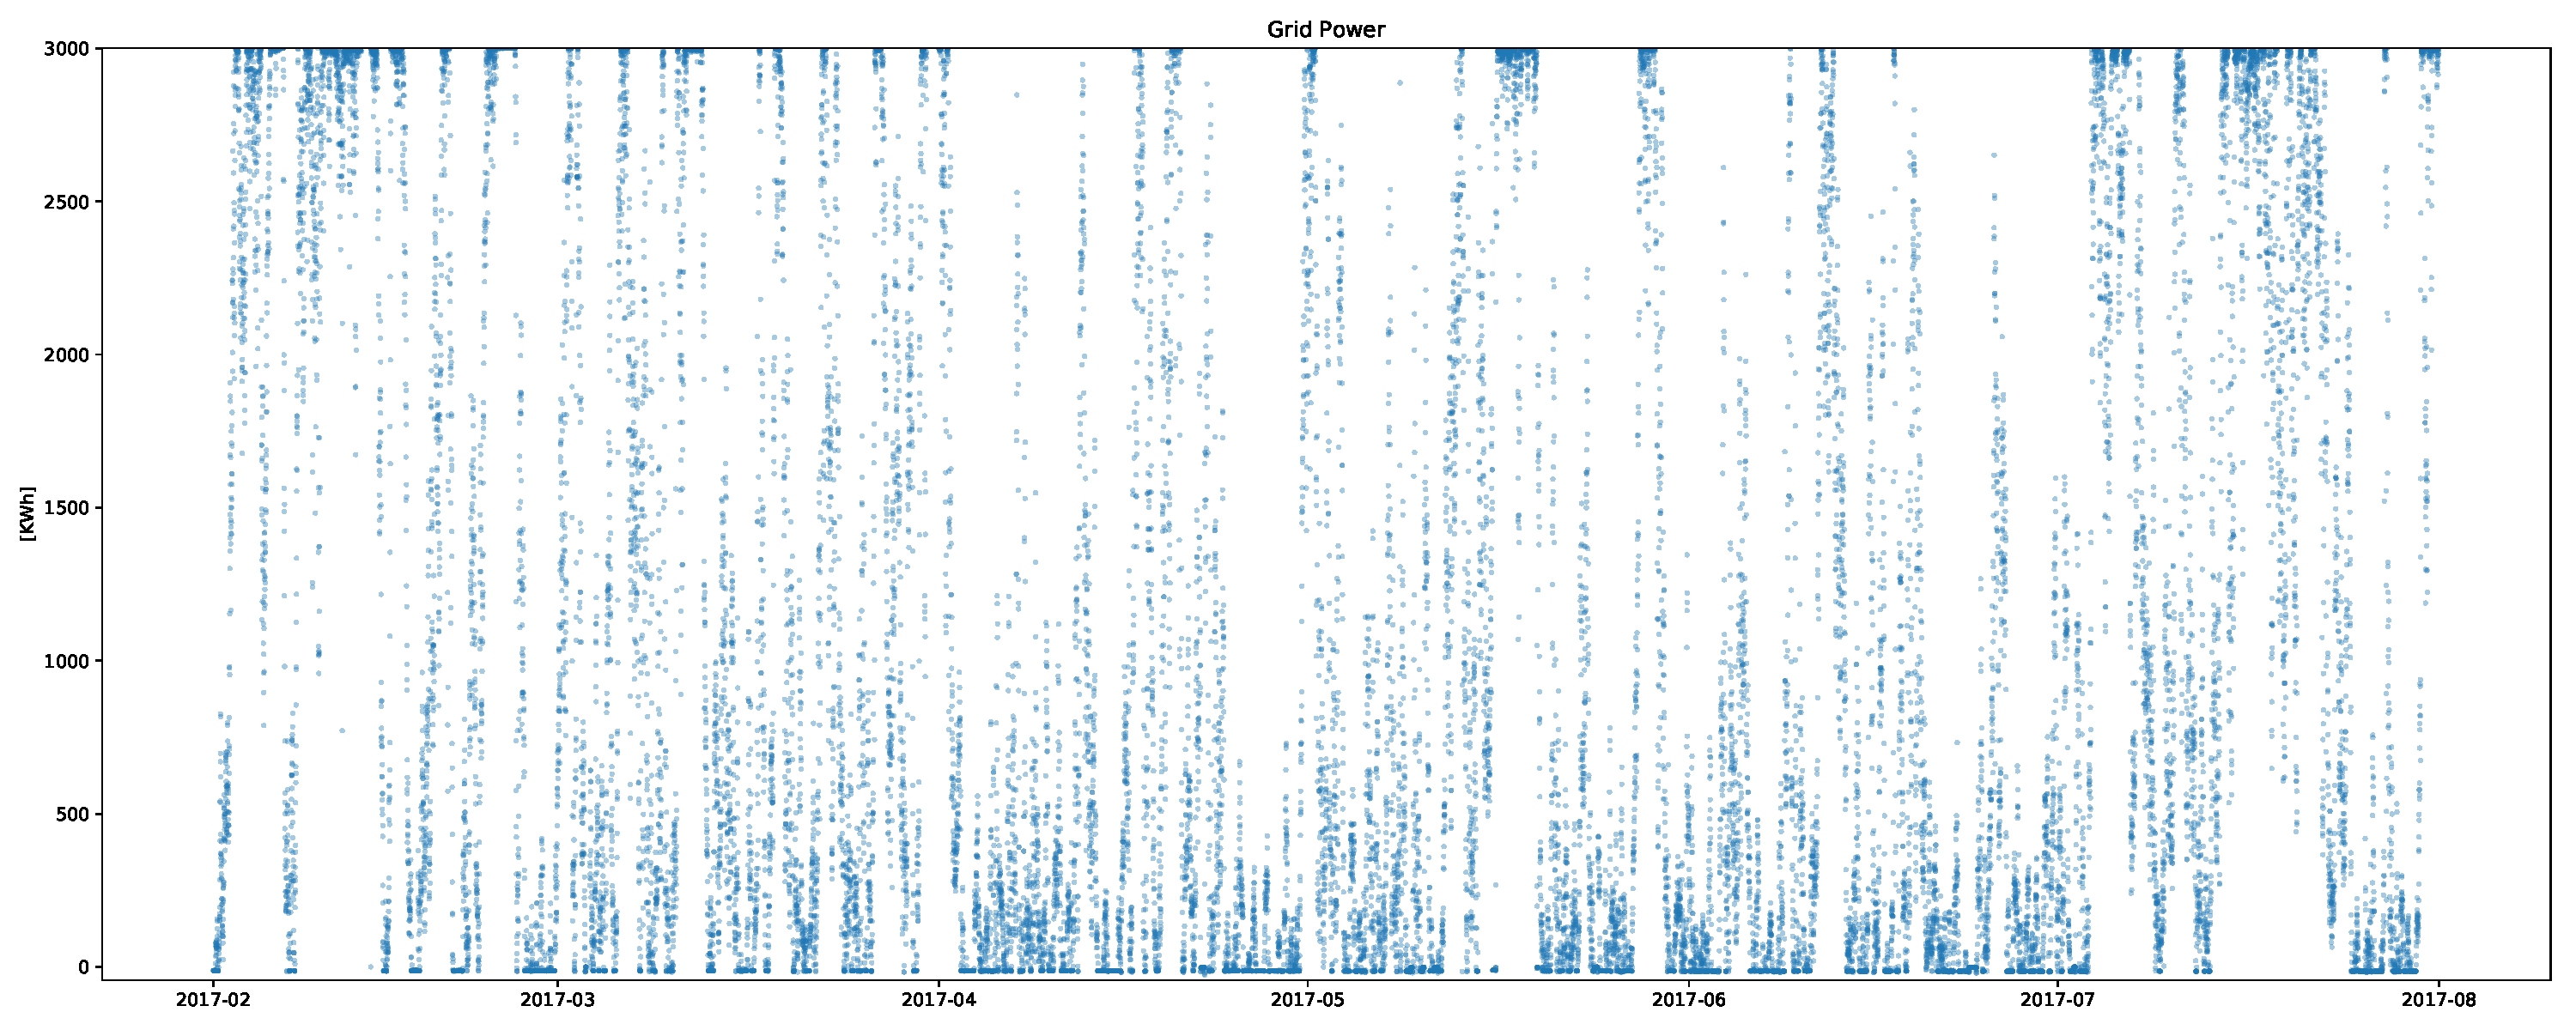
\includegraphics[width=0.9\textwidth]{grid_power.pdf}
        \label{fig:grid_power}
    }
    \caption{Individual sequential graphs for the sensory information}
    \label{fig:data}
\end{figure}

In this dataset, wind speed can be seen as an input to the system while the rotor speed and the generated power are the outputs of the system. However, it can be seen from Figure~\ref{fig:data} that there is not a direct relationship between these features. The reason behind this phenomena is that previous observations and working condition of the turbine affect the current time observations because of the physical relationships in the mechanical system of the wind turbines. Therefore, the outputs cannot be generated directly according to input data, and it requires the system state, which indicates how the system reacts to the given input. 
The interaction graph which is obtained from a limited time interval and does not consider the time series feature can be seen in Figure~\ref{fig:powercurve}.

\begin{figure}
    \centering
    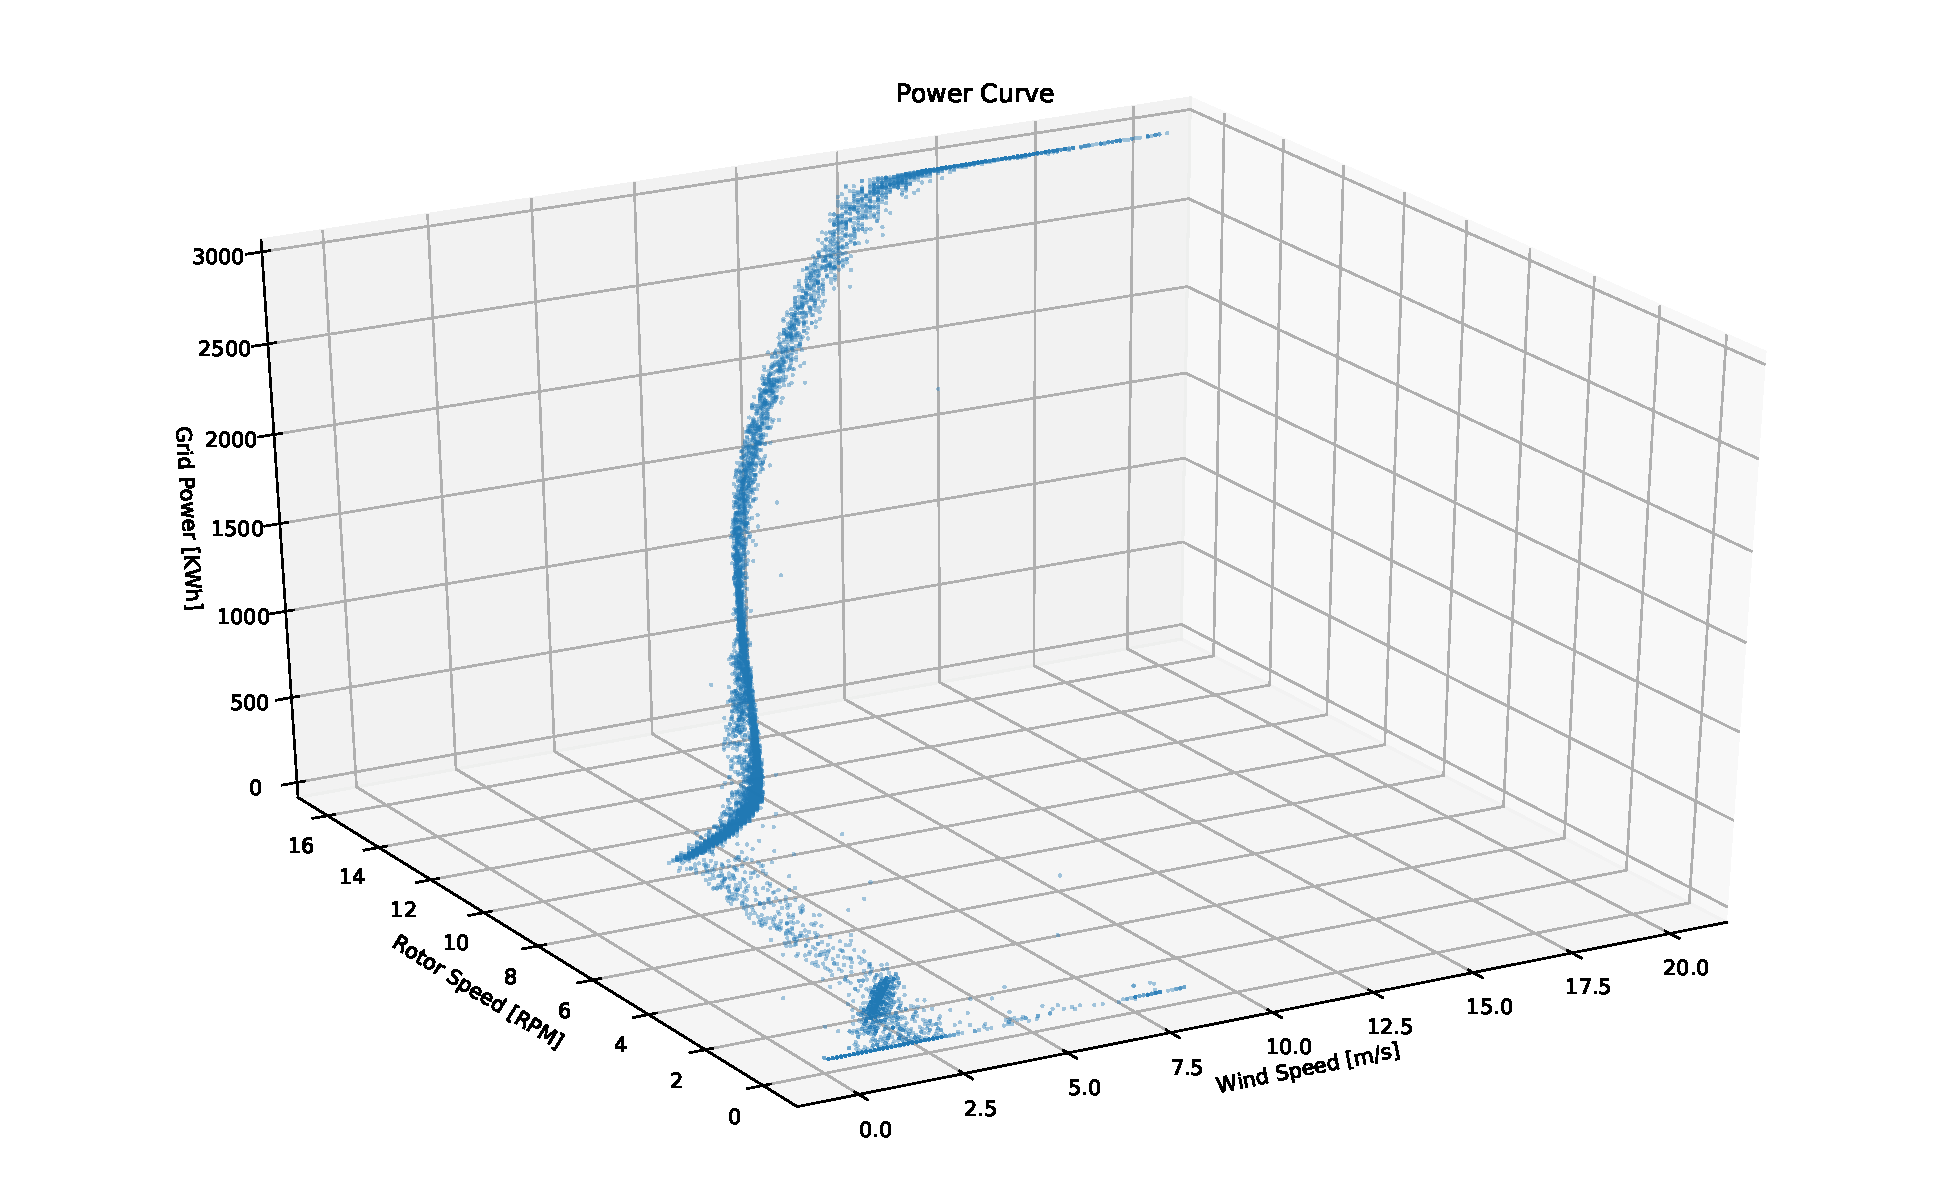
\includegraphics[width=\textwidth]{power.pdf}
    \caption{The relationship between the wind speed, rotor speed and grid power}
    \label{fig:powercurve}
\end{figure}

\subsection{Modeling The Power Curve of Wind Turbine}

The power curve of wind turbines defines the relationship of a wind speed or rotor speed, or both, to the amount of power generation. Since, the physical machinery has a sophisticated control mechanism, as well as environmental variations that are not directly measurable, makes this relationship more complicated. Therefore, we have to create a model that works under different circumstances according to basic working principals of the wind turbines. For this purpose, we use Bayesian approaches to generate the power curve of the wind turbine efficiently.

There are different approaches to the modeling of the power curve. Some of the works use wind speed and grid power to evaluate the power curve \cite{ouyang:17} and some other uses rotor speed and grid power to evaluate power curve \cite{romero:16}. On the other hand, we use both rotor speed and wind speed because only wind cannot give too much information because it has too much uncertainty and there is a lot of sudden changes in the wind speed. On the other hand, rotor speed itself again cannot give desired results because there is break points in the rotor speed - power curve graph. In addition to that, such a discontinuity is not desired in such a model. Therefore we use both wind speed and rotor speed to analyze power curve model. By this selection, we see that the discontinuity in the rotor speed - grid power model is gone, and the high variance in the wind speed - power curve is also reduced. Therefore increasing the dimensionality of the power curve significantly strengthens our hands in terms of better analysis.

The power curve shows us the critical features of the wind turbine machinery system. However, although the wind speed, rotor speed, and grid power are included, the turbine still contains some discontinuity in the power curve as a result of some states of the turbine. Since there is a gearbox in the turbine, we expect that kind of relationship, and we can see the location of this change points from the power curve.

In addition to the previous details, we can also add the time factor to the account. When we do this, we create the power curve using the incoming data sequence. On this page, we can analyze not only the power curve but also the trends of change on the power curve.

We aim to find the optimum power curve for each turbine individually because the physical machines are complex systems, and even if they work with precisely the same mechanism, they can show different production values. The power curve includes the main line that the turbine is likely to generate and the variance that occurs. It is important to note that since wind turbines are rotating systems, the variance of the production will increase with the rotor speed. Therefore our model should take into account that property.

\subsection{Experiments with the Probabilistic Models}

We started this study by reconstruction of the power curves of the wind turbines using \textit {Gaussian Mixture Model}(GMM).
This model learns the power curve of the wind turbine as a mixture of Gaussian distribution over the available data. 
At this point, we assume that our observations include both turbine states and anomalies.
Therefore we assume that, in the model, there are $10$ different Gaussian distributions for turbine operation states which should be learned and there is $1$ Gaussian distribution with the infinite variance, uniform over output space, for sensory information errors or anomalies. 
These Gaussian distributions are then learned using the EM algorithm, except the distribution corresponds to anomalies.
Once the distributions are learned, we can determine which distribution the incoming data belongs to, and what observations are anomalies.
Therefore, according to this model, the incoming data has a predictive error rate. 
This model, which is more straightforward than HMM, does not take into account the time effect and how the consecutive observations should behave is not taken into account.
Therefore, the Gaussian distributions in the model are learned without this knowledge.
Since the incoming data is not analyzed as a time series, the model is more susceptible to faulty data coming from the sensors and can not catch the faulty transitions between states. The mixtures are shown in Figure~\ref{fig:gmm-mixtures}. Moreover, the model may be insufficient to detect unexpected fluctuations in the power output of the turbine.

\begin{figure}
\centering
    \subfigure[The mixture of Gaussians]{
        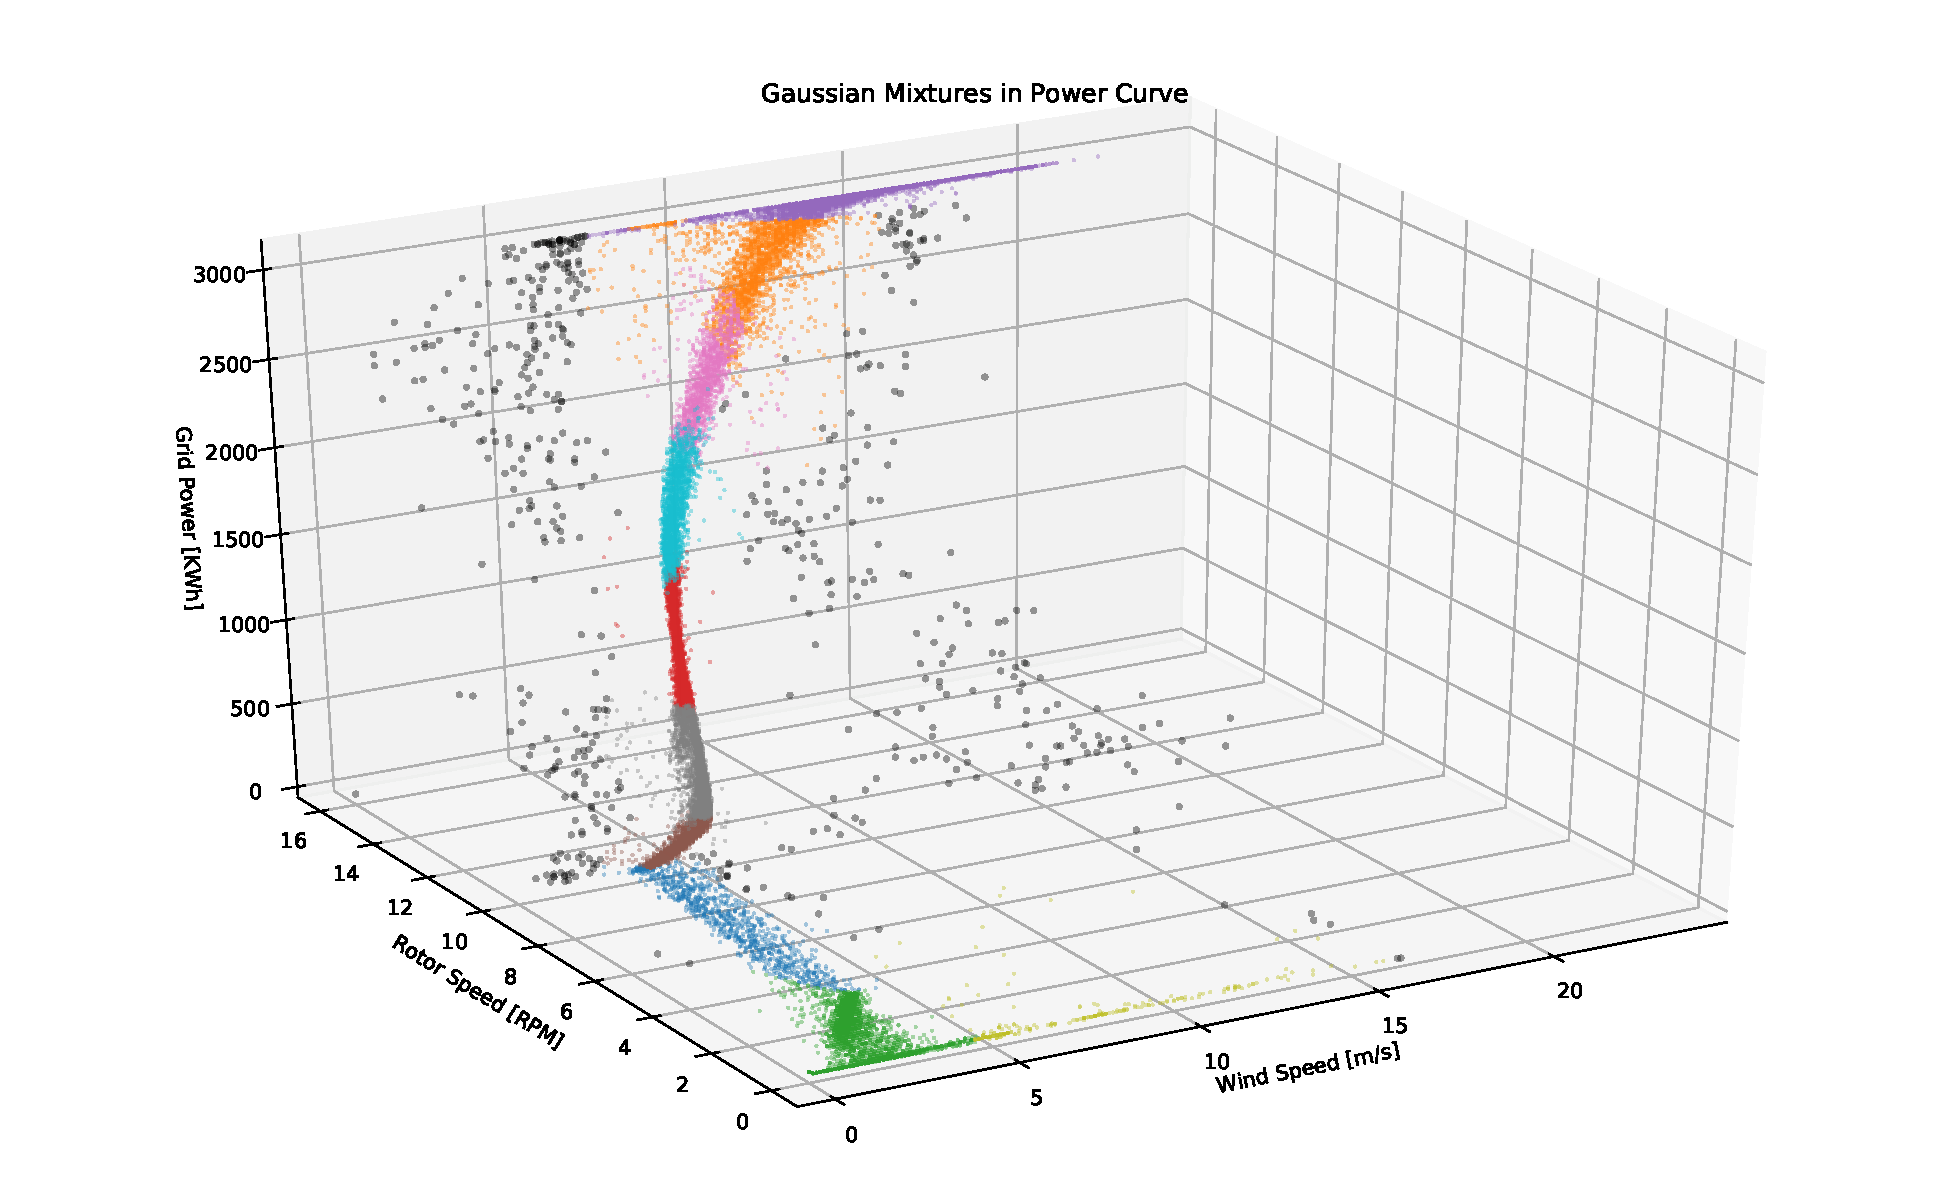
\includegraphics[width=0.95\textwidth]{gmm-mixtures.pdf}
        \label{fig:gmm-mixtures}
    }%
    
    \subfigure[Distributions in the latent space]{
        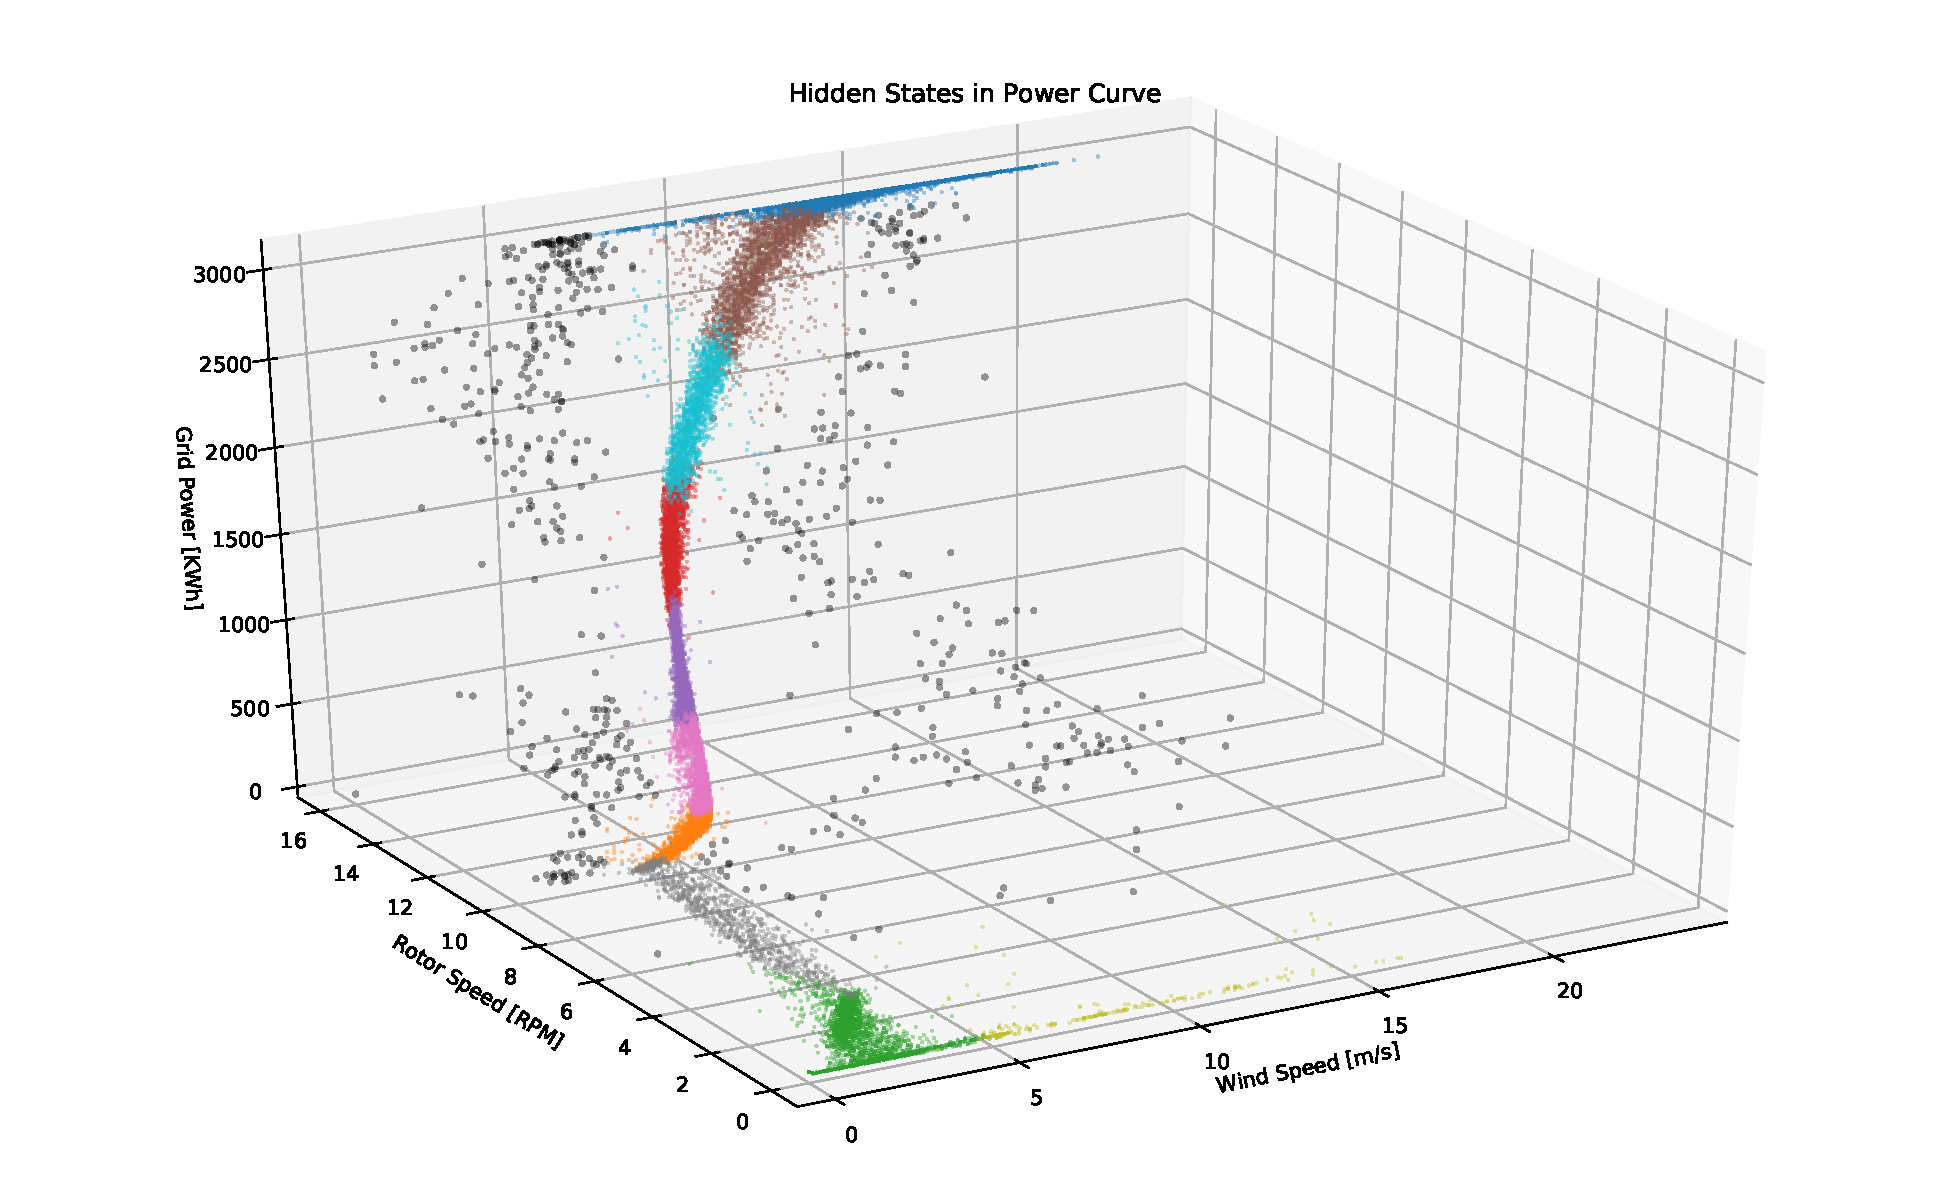
\includegraphics[width=0.95\textwidth]{hmm-mixtures.pdf}
        \label{fig:hmm-mixtures}
    }

    \caption{Comparison of the mixture of Gaussians in the GMM with distributions in the latent space of the HMM on the power curve.}
    \label{fig:mixtures}
\end{figure}

In the expanse of this study, the power curves of the wind turbines are constructed as time series using HMM. 
This model also learns the power curve of the wind turbine as a mixture of Gaussian distribution over the available data. 
Therefore we assume that, as in GMM, there are $10$ different Gaussian distributions for turbine operation states which should be learned and there is $1$ Gaussian distribution with the infinite variance, uniform over output space, for sensory information errors or anomalies. 
We design our model in such a way as to determine which distribution will come from which distribution.
Therefore, the previous distribution will have an impact on the distribution of the observations. Therefore the learned mixtures of the Gaussian distributions of the states will be slightly different from that obtained in the GMM.
The learned Gaussian mixtures by HMM are shown in Figure~\ref{fig:hmm-mixtures}. 
The better modeling of the system, as can be seen in Figure~\ref{fig:mixtures} has resulted in more obvious mixtures.
This model was trained by processing the sample mini-series of $144$ measurements, which corresponds to one-day observations. 
During this training, the learning speed was chosen as $\eta_t=1/\left(t+1\right)$. 
On the other hand, the state transition diagram of the HMM is shown in Figure~\ref{fig:transition}.
As can be seen from the transition diagram, it is possible to switch from any state to anomaly.
Therefore, the HMM model is more tolerant to incorrect measurements from the detectors and can detect abnormal changes in the power curve without being affected by false observations as it learns the operation of the turbine.
As a result of these studies, it can be seen that HMM can make error prediction more clear than GMM, according to Figure~\ref{fig:hmm-figc} and Figure~\ref{fig:hmm-figd}. However, the most critical point of HMM is that it minimizes the false positive error prediction. In most cases, the GMM tends to produce false positive predictions, as shown in Figure~\ref{fig:hmm-figf}, but HMM has achieved much better results in this regard. A detailed comparison between GMM and HMM model is given in Figure~\ref{fig:hmm-results}. Malfunctions are shown as black vertical lines in graphs. The collective anomaly result is cumulatively calculated from the anomaly forecast for each observation and converted into a warning signal.

\begin{figure}
    \centering
    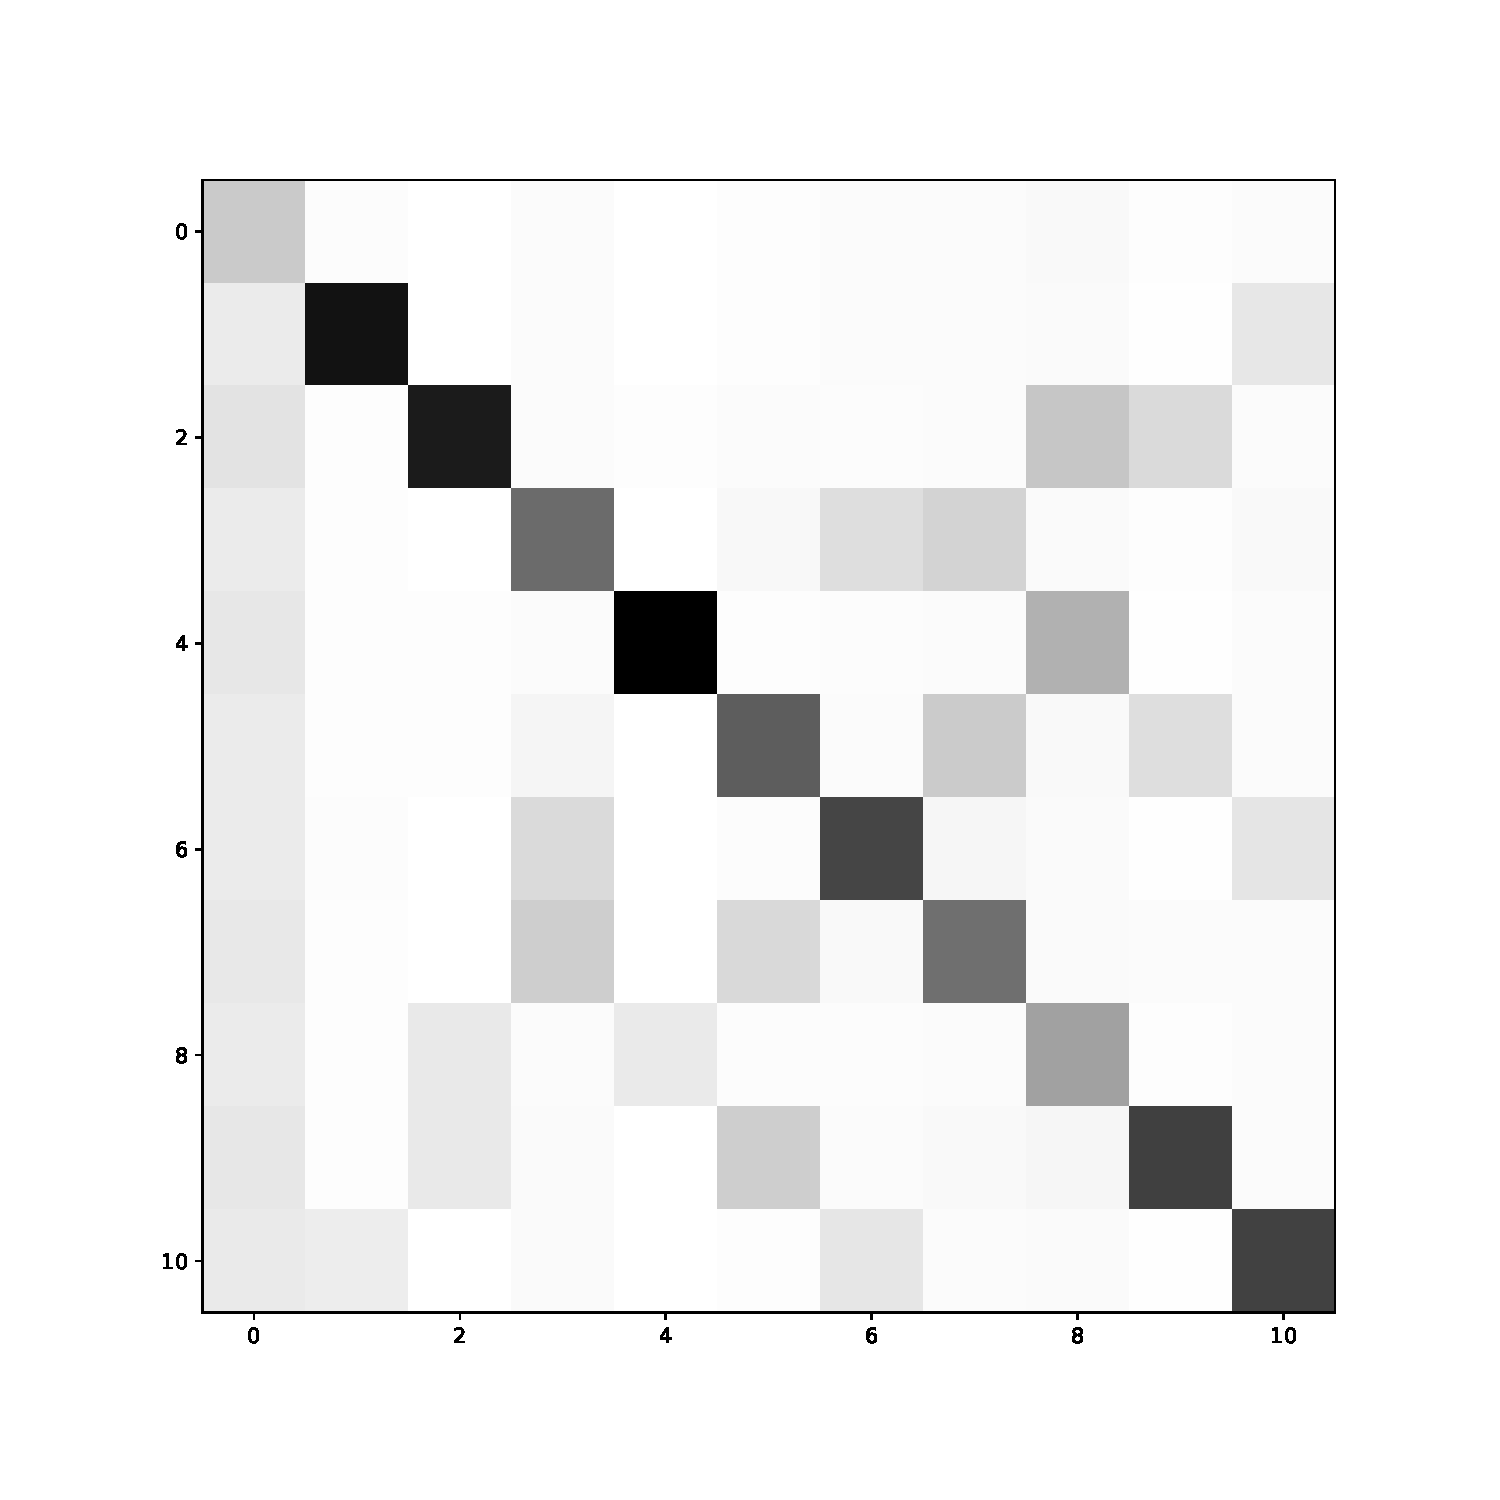
\includegraphics[width=0.6\textwidth]{transition.pdf}
    \caption{State transition diagram of the HMM}
    \label{fig:transition}
\end{figure}

\begin{figure}
    \centering
  \subfigure[The error prediction of HMM on the turbine which works under normal conditions]{
       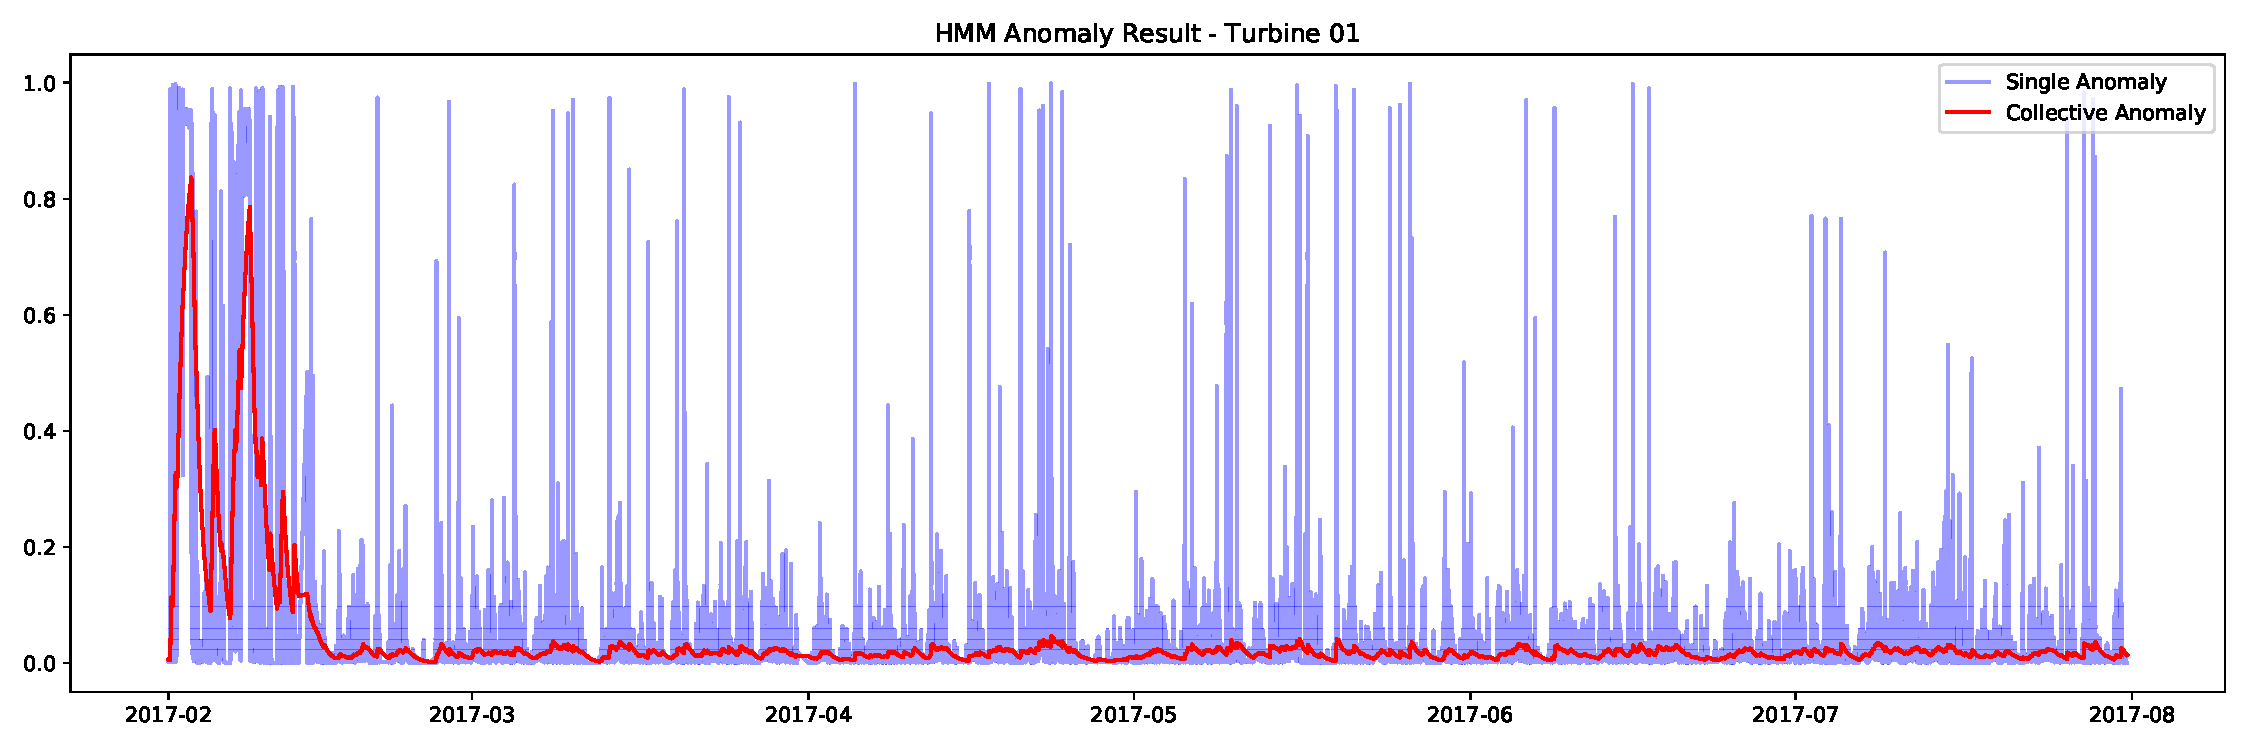
\includegraphics[width=0.48\textwidth]{hmm_t1.pdf}
       \label{fig:hmm-figa}
    }%
  \hfill
  \subfigure[The error prediction of GMM on the turbine which work under normal conditions]{
       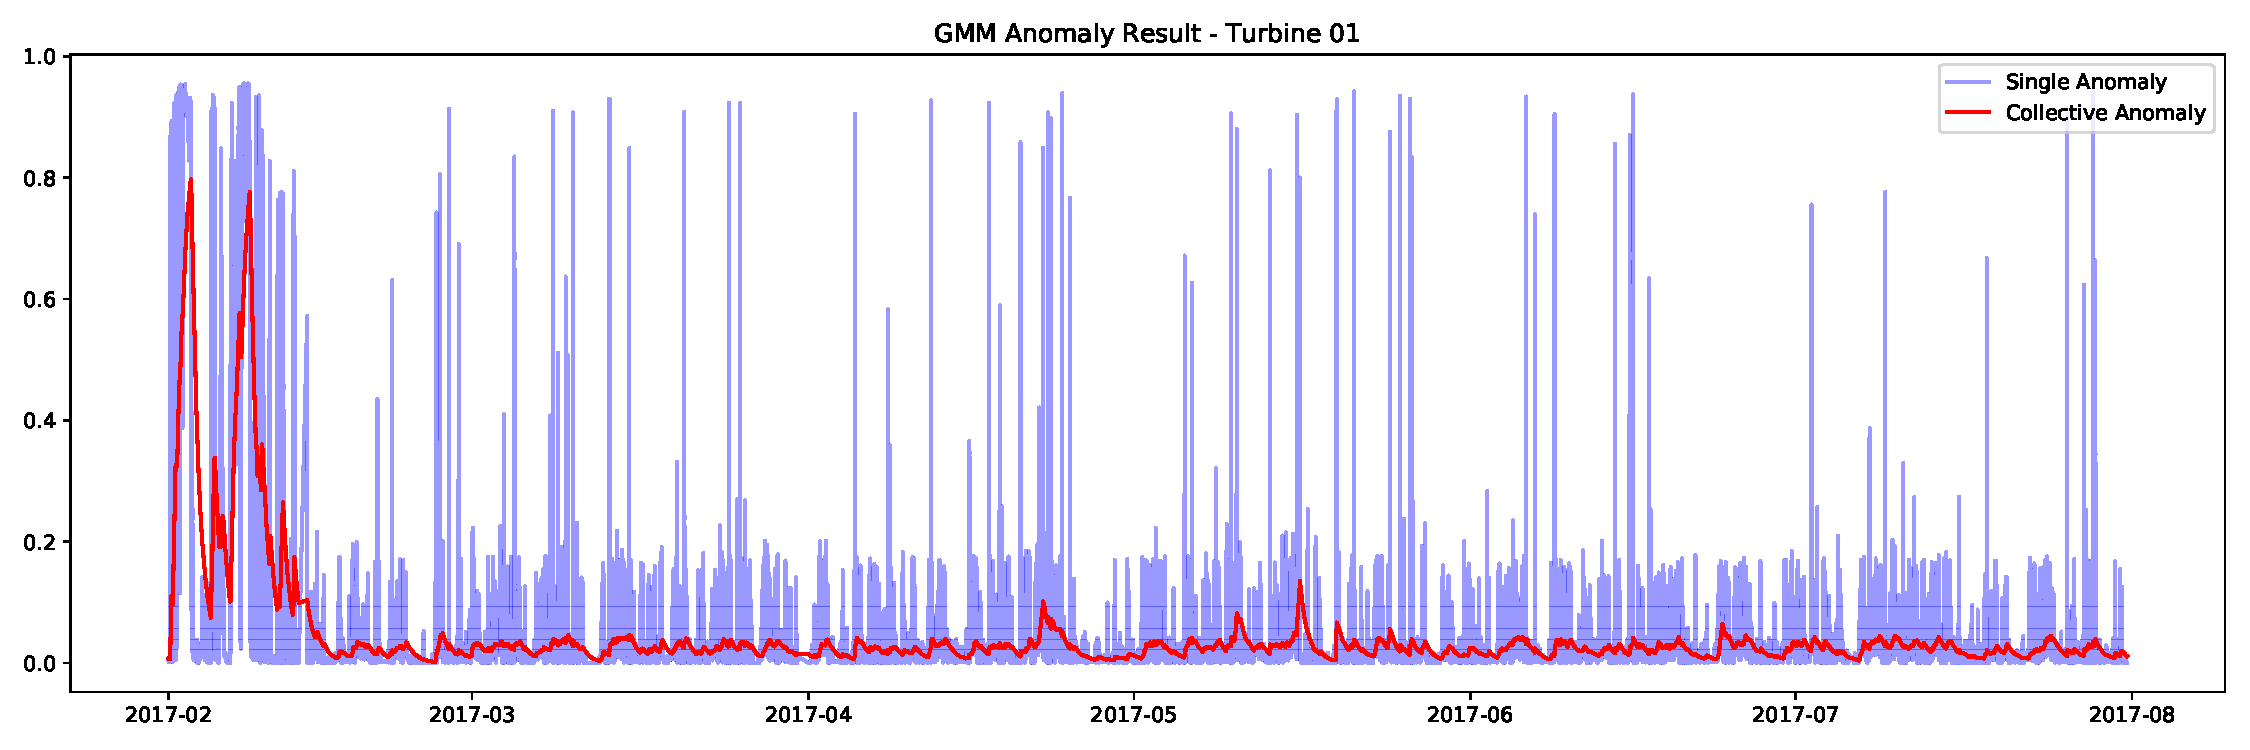
\includegraphics[width=0.48\textwidth]{gmm_t1.pdf}
       \label{fig:hmm-figb}
  }
  
  \subfigure[HMM generates two clear warning before malfunction on the June]{
       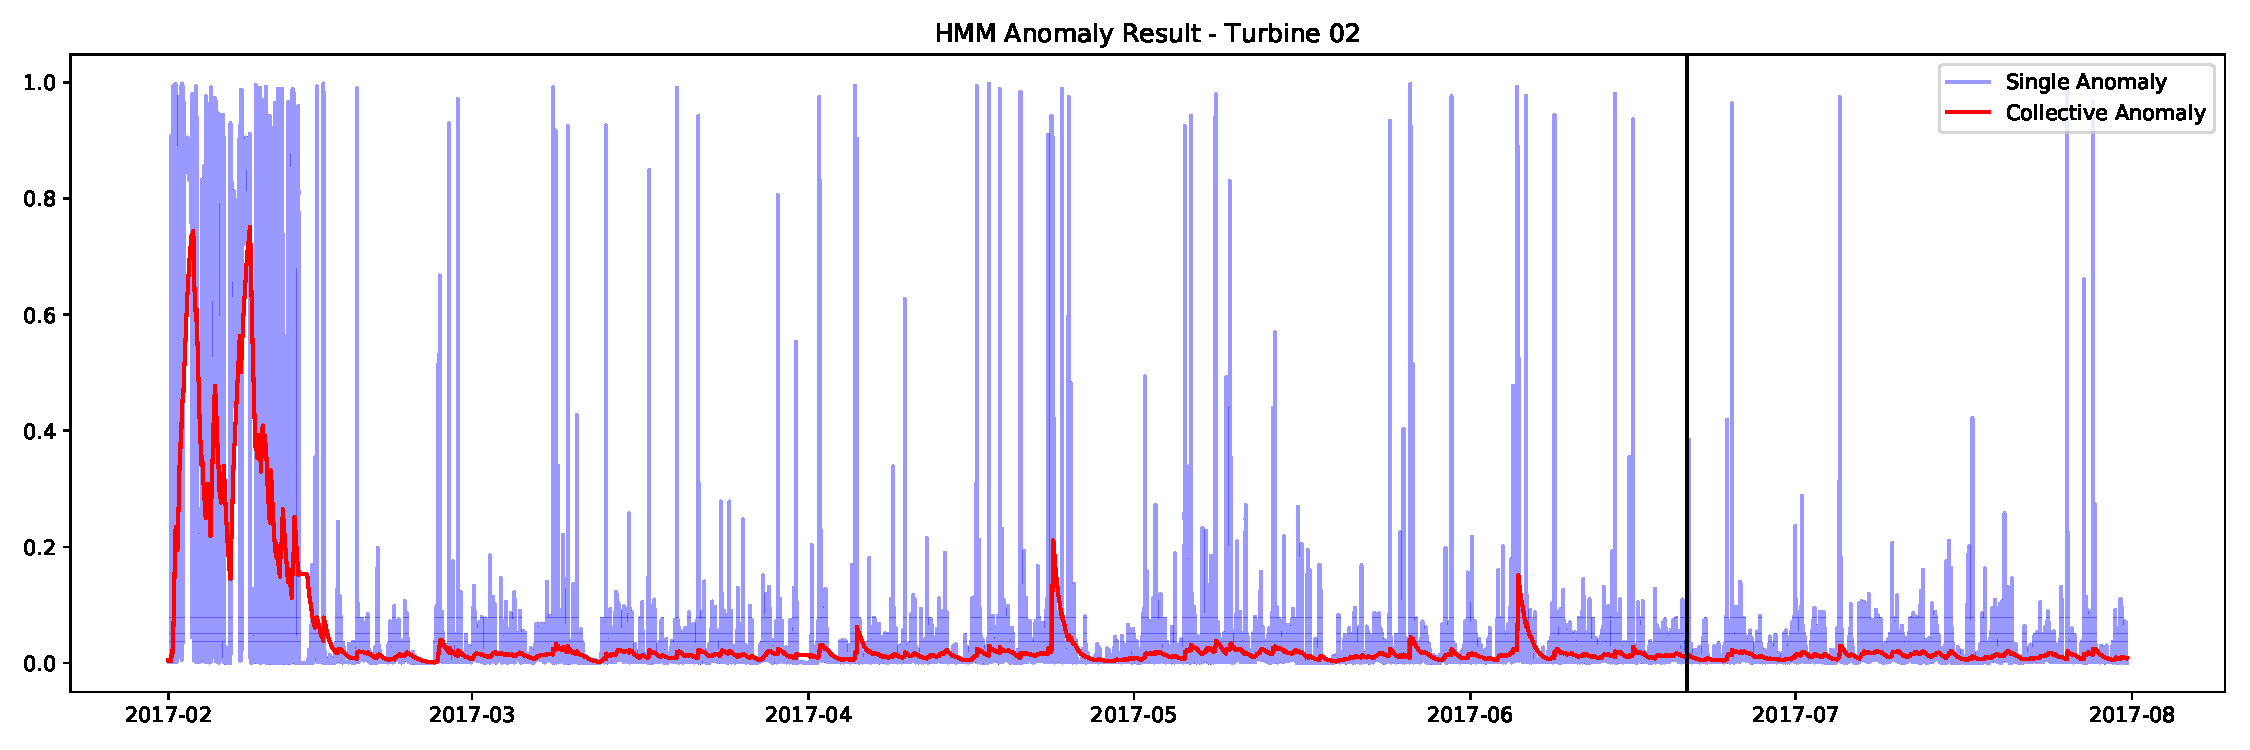
\includegraphics[width=0.48\textwidth]{hmm_t2.pdf}
       \label{fig:hmm-figc}
  }%
  \hfill
  \subfigure[Warnings of GMM are not clear as warning generated by HMM]{
       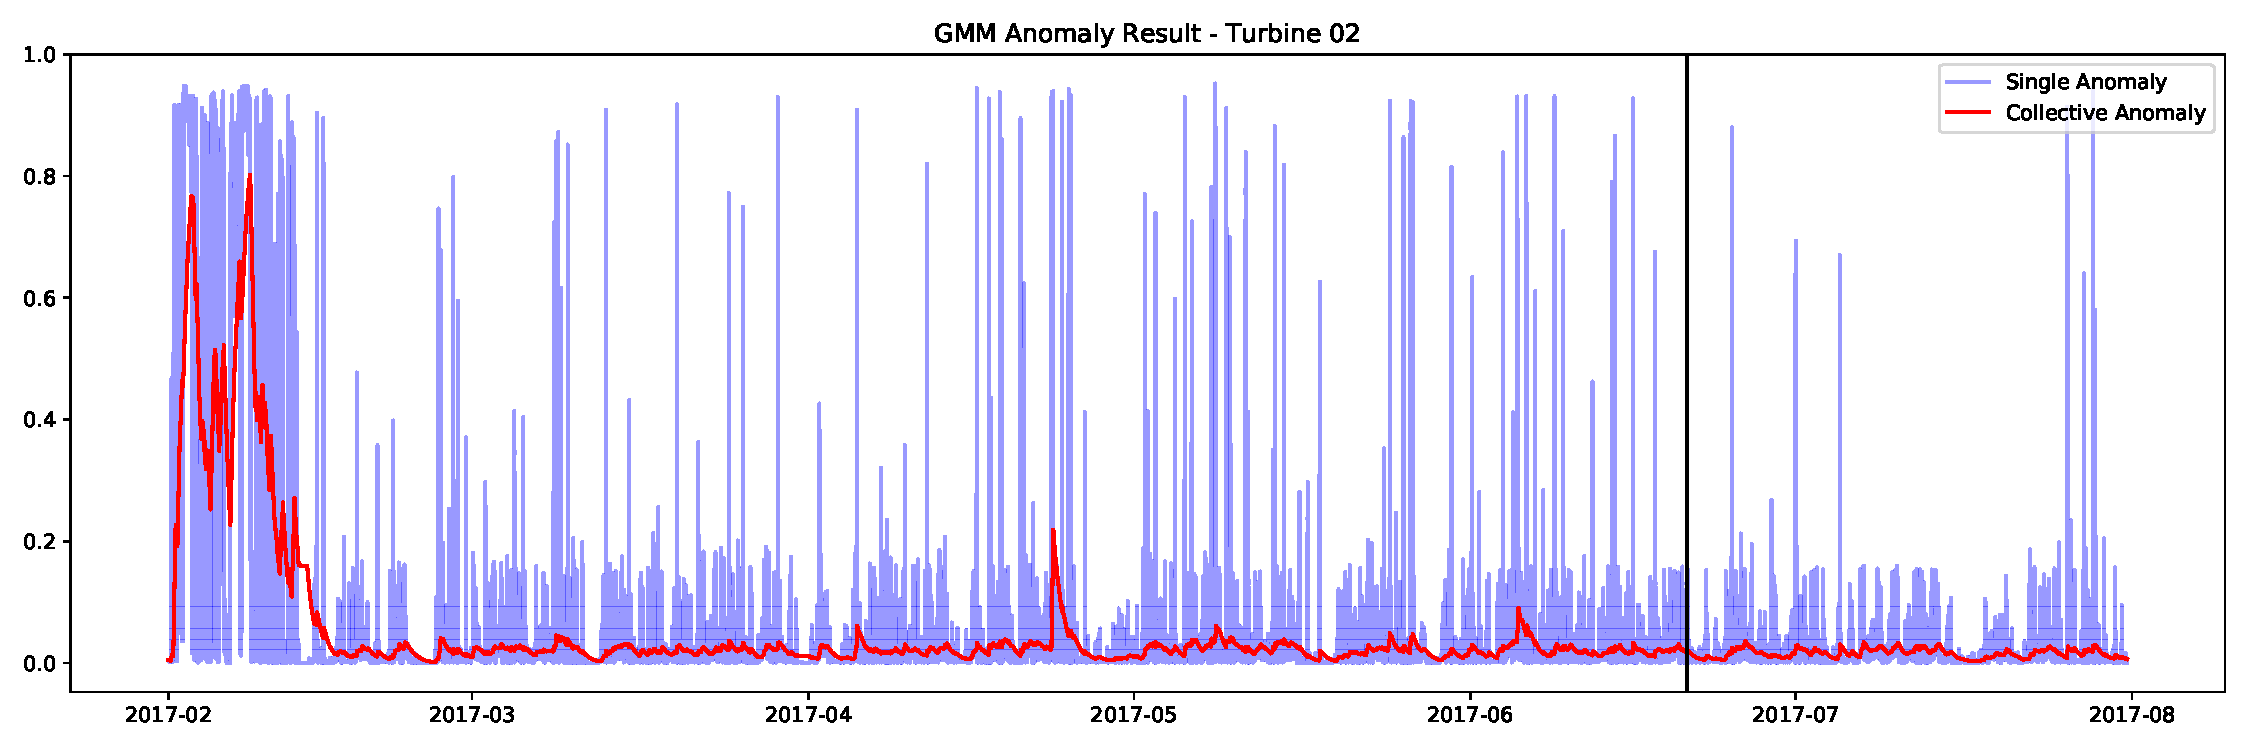
\includegraphics[width=0.48\textwidth]{gmm_t2.pdf}
        \label{fig:hmm-figd}
  }
  
  \subfigure[HMM does not predict error for the turbine which works under normal conditions]{
       %\centering
       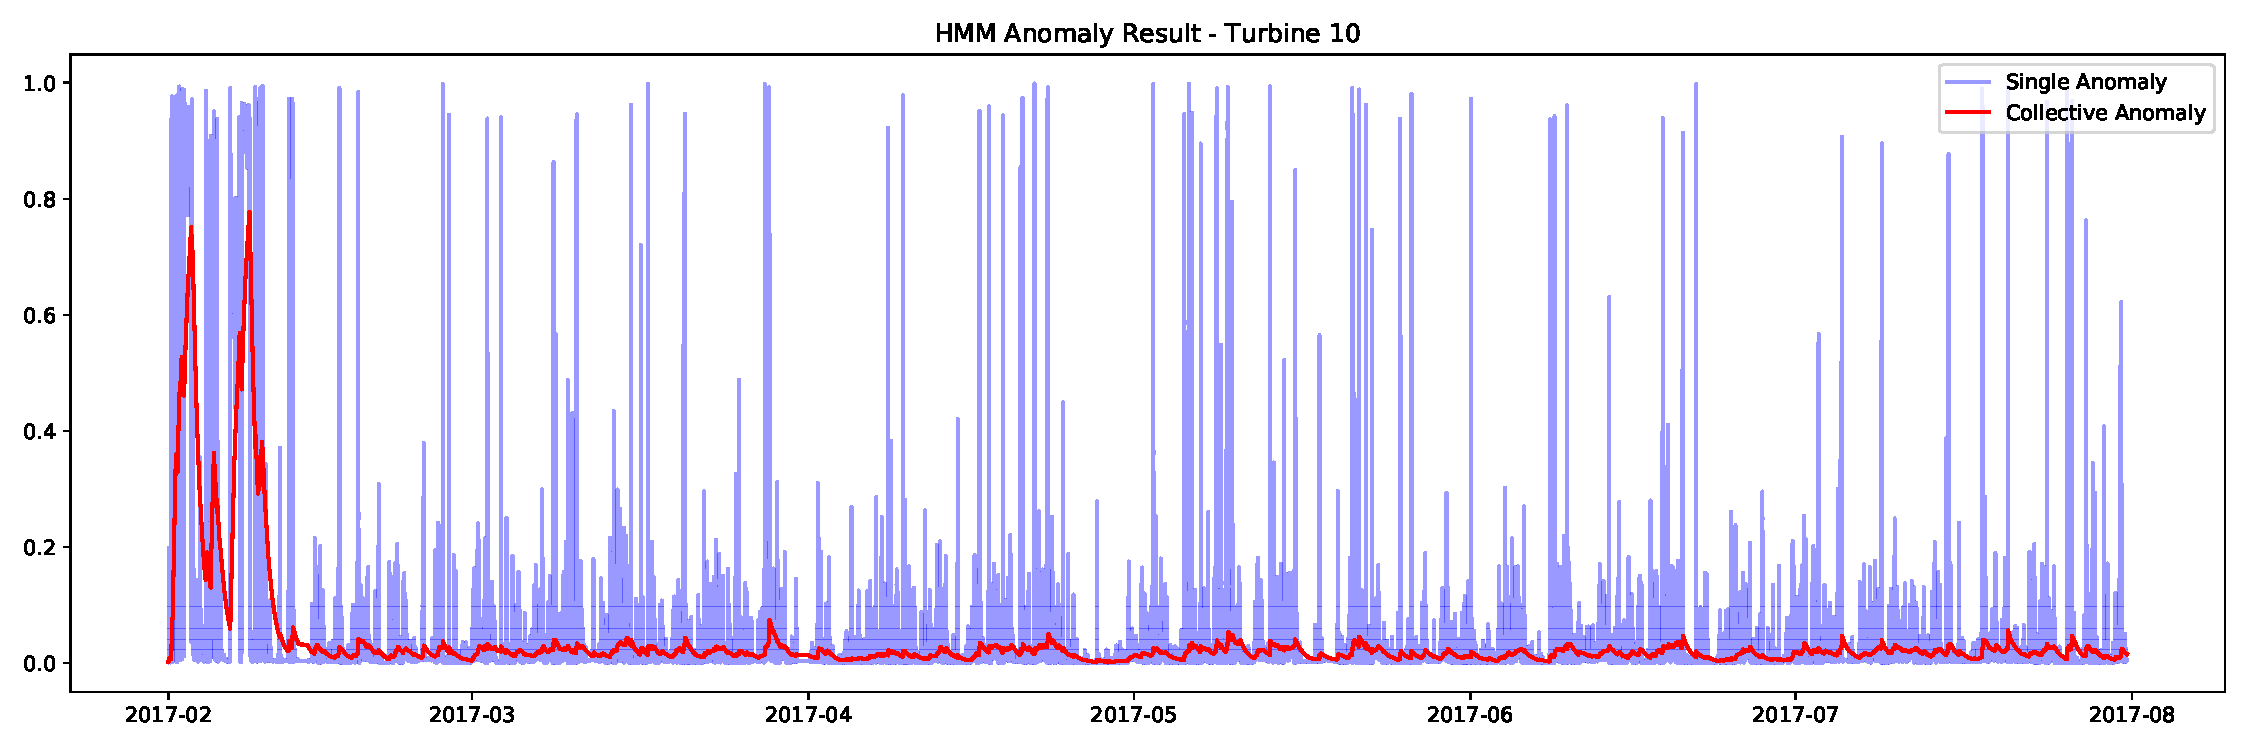
\includegraphics[width=0.48\textwidth]{hmm_t10.pdf}
        \label{fig:hmm-fige}
  }%
  \hfill
  \subfigure[GMMs tend to produce false positive warnings on the normally working turbine]{
       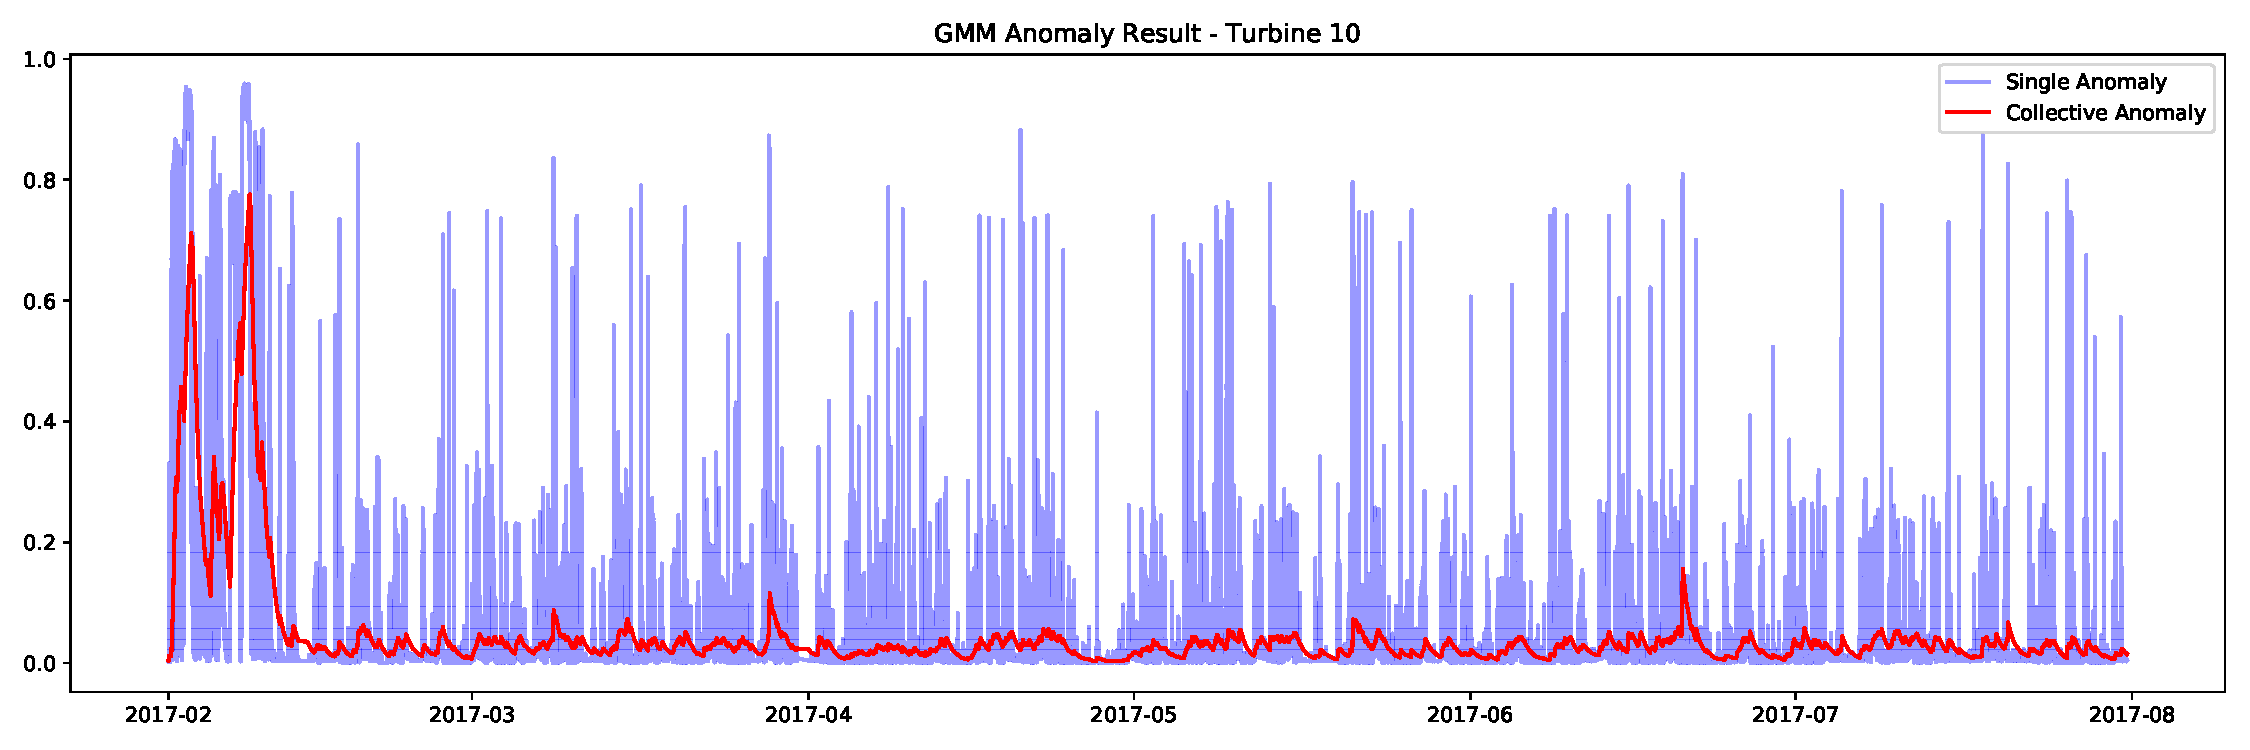
\includegraphics[width=0.48\textwidth]{gmm_t10.pdf}
       \label{fig:hmm-figf}
  }
  \caption{Comparison of the performance of HMM with GMM}
  \label{fig:hmm-results}
\end{figure}

\subsection{Experiments with the Deep Learning Sequence Models}

In this part of the study, we are interested in deep learning models to detect anomalies. 
Therefore we apply such models to the power curve of the wind turbines to learn about the system dynamics.
The main idea behind this study is to reconstruct the power curve of the wind turbines with developed models.
Then, in the test phase, we will first reconstruct the power curve, and compare this reconstruction with the new observations and measure how wrong they are.
This measurement will also determine our anomaly score.
In the experimental setup, we basically compare the RNN network with LSTM network.
While making this comparison, we will do our experiments by changing two additional parameters.
The first parameter to examine the effect on the model is the depth of the network.
For both RNN and LSTM, we compare the results with $1$-layer network with $2$-layer network (stacked) \cite{malhotra2015long}.
The other parameter to examine the effect on the model is loss function.
We examine the effect of the L1 loss and MSE loss on the developed model.
We focus on these two losses because both models have the rectified linear output layer, and these loss functions are more appropriate for such a model. 
In the rest of the experimental setup, we set all hyperparameters to the same for the healthy comparison.
We set learning rate $\eta = 0.01$ for all of the network setups, and we train each network for $1000$ number of the epoch. All the experimental setups use the same batch size, $144$ observation time-step for one batch. In the experiments, both RNN and LSTM network has the number of hidden layer size $128$.

\begin{figure}
\centering
    \subfigure{
        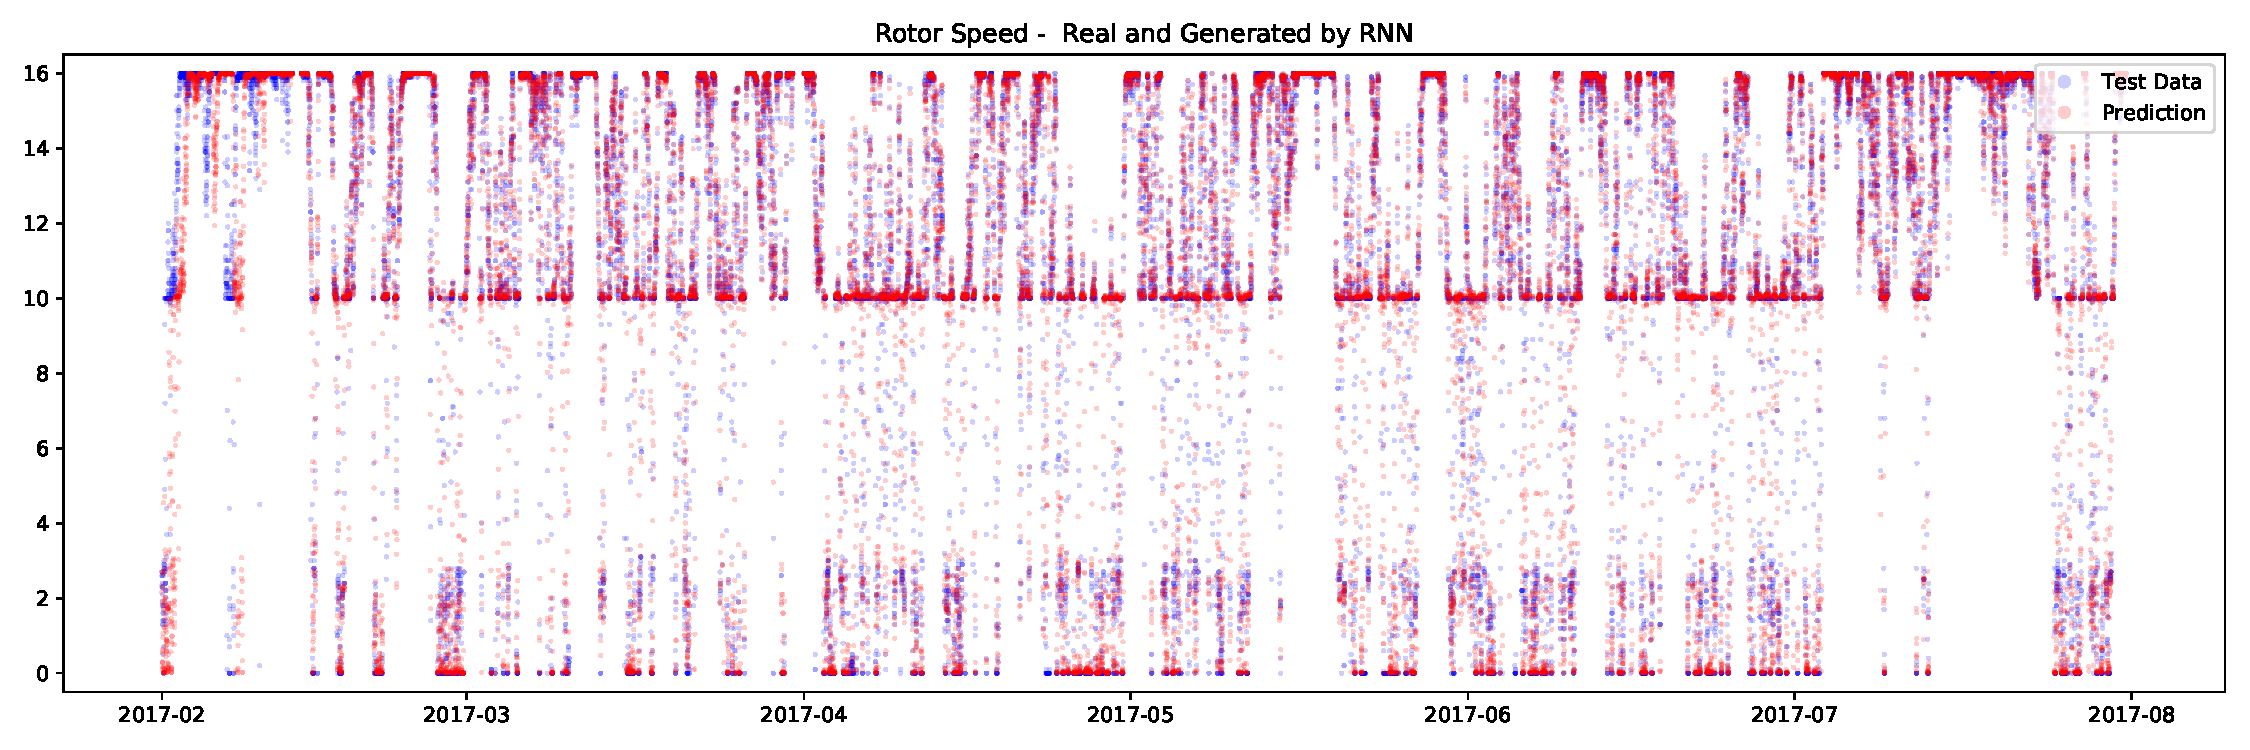
\includegraphics[width=0.9\textwidth]{rnn_rotor_128_2_tukey.pdf}
        \label{fig:rnn_rotor}
    }%
    
    \subfigure{
        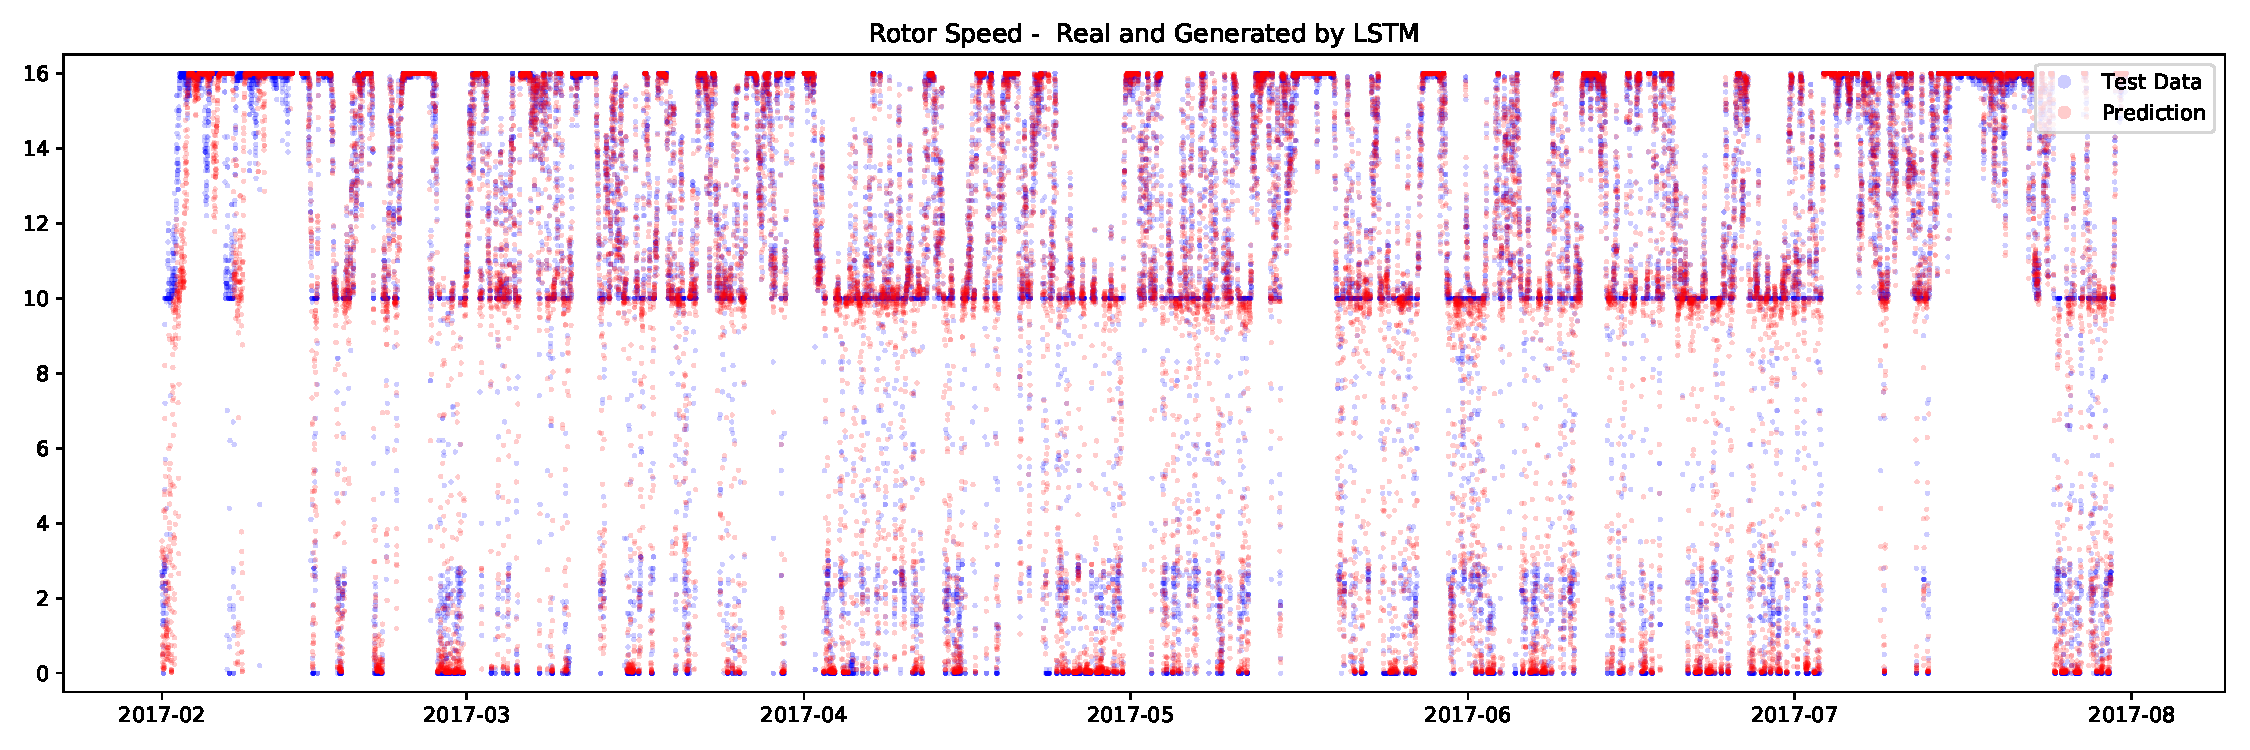
\includegraphics[width=0.9\textwidth]{lstm_rotor_128_2_tukey.pdf}
        \label{fig:lstm_rotor}
    }
    
    \caption{Predicted rotor speed data for RNN and LSTM model with Tukey's biweight loss}
    \label{fig:deep_rotors}
\end{figure}

In these experiments, we implement $12$ different experiment setup. 
These setups include RNN or LSTM, $1$-layer or $2$-layer, and L1 loss or MSE loss or Tukey's biweight loss.
Our experiments show that both RNN and LSTM setups have almost similar performance on the system.
This is because wind turbine dataset does not contain long-term dependencies and to obtain good estimation we do not need to know information from the future. 
On the other side, experiments show us that stacked networks perform better on the power curves.
This situation may be due to the complexity of the power curve.
Finally, we see in the experiments that L1 loss is a better choice to model such data because data includes anomalous observations and MSE loss not robust for such observations while L1 does.
Tukey's biweight loss, on the other hand, allow us to perform more robust optimizations and perform better on our task.
These networks almost totally correctly estimate the generated power and rotor speed values from the given wind speed, as in Figure~\ref{fig:deep_rotors}, Figure~\ref{fig:deep_powers}, Figure~\ref{fig:1-deep_power_curves} and Figure~\ref{fig:2-deep_power_curves}. 
The first two figures are generated from the stacked RNN and stacked LSTM network with the Tuckey's biweight loss.
Except for a small difference, both the RNN and LSTM model creates almost the same predictions on rotor speed and grid power values.
The third figure includes generated power curves for all experimental setups. In all figures, blue dots represent the observations while red dots show the model outputs.
In Figure~\ref{fig:1-deep_power_curves}, one can detailly analyze the performance of the 1-layer models with a different setting.
Similarly, in Figure~\ref{fig:2-deep_power_curves}, we share the performance of stacked (2-layered) networks.
Despite their small differences, all models produced acceptable results and found almost the same anomaly result. The anomaly scores are shown in Figure~\ref{fig:1-deep_anomalies} and Figure~\ref{fig:2-deep_anomalies}. 
Black vertical lines in the figures represent the malfunction in turbines, and the system generates warning before the malfunction.
Additionally, we know that at the February there is an iciness on the turbines. 
Models successfully detect these anomalies in all experiments.
These figures show that the results are very similar to each other and also similar to the ones that we find with probabilistic models in Figure~\ref{fig:hmm-results}.
Detailed analysis of the 1-layer networks can be found in Figure~\ref{fig:1-deep_anomalies}, while Figure~\ref{fig:2-deep_anomalies} includes detailed analysis of the 2-layer (stacked) networks.
In both experiments, blue dots represent the observations while red dots represent the predictions.

\begin{figure}
\centering
    \subfigure{
        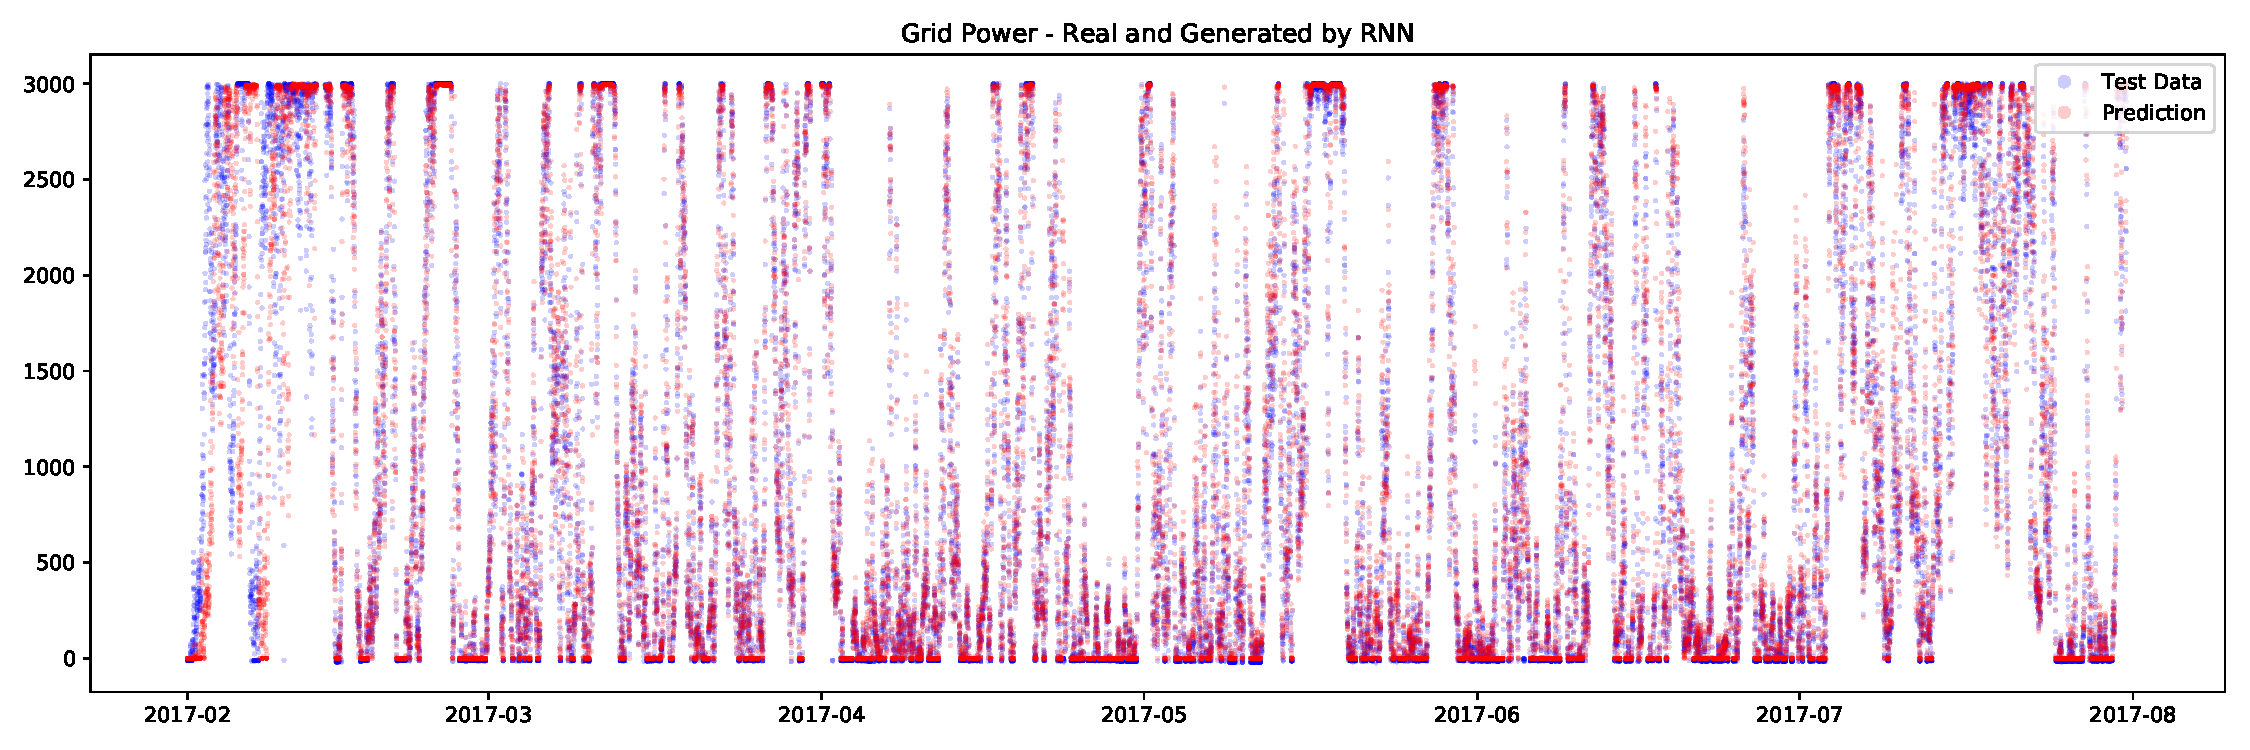
\includegraphics[width=0.9\textwidth]{rnn_grid_power_128_2_tukey.pdf}
        \label{fig:rnn_power}
    }%
    
    \subfigure{
        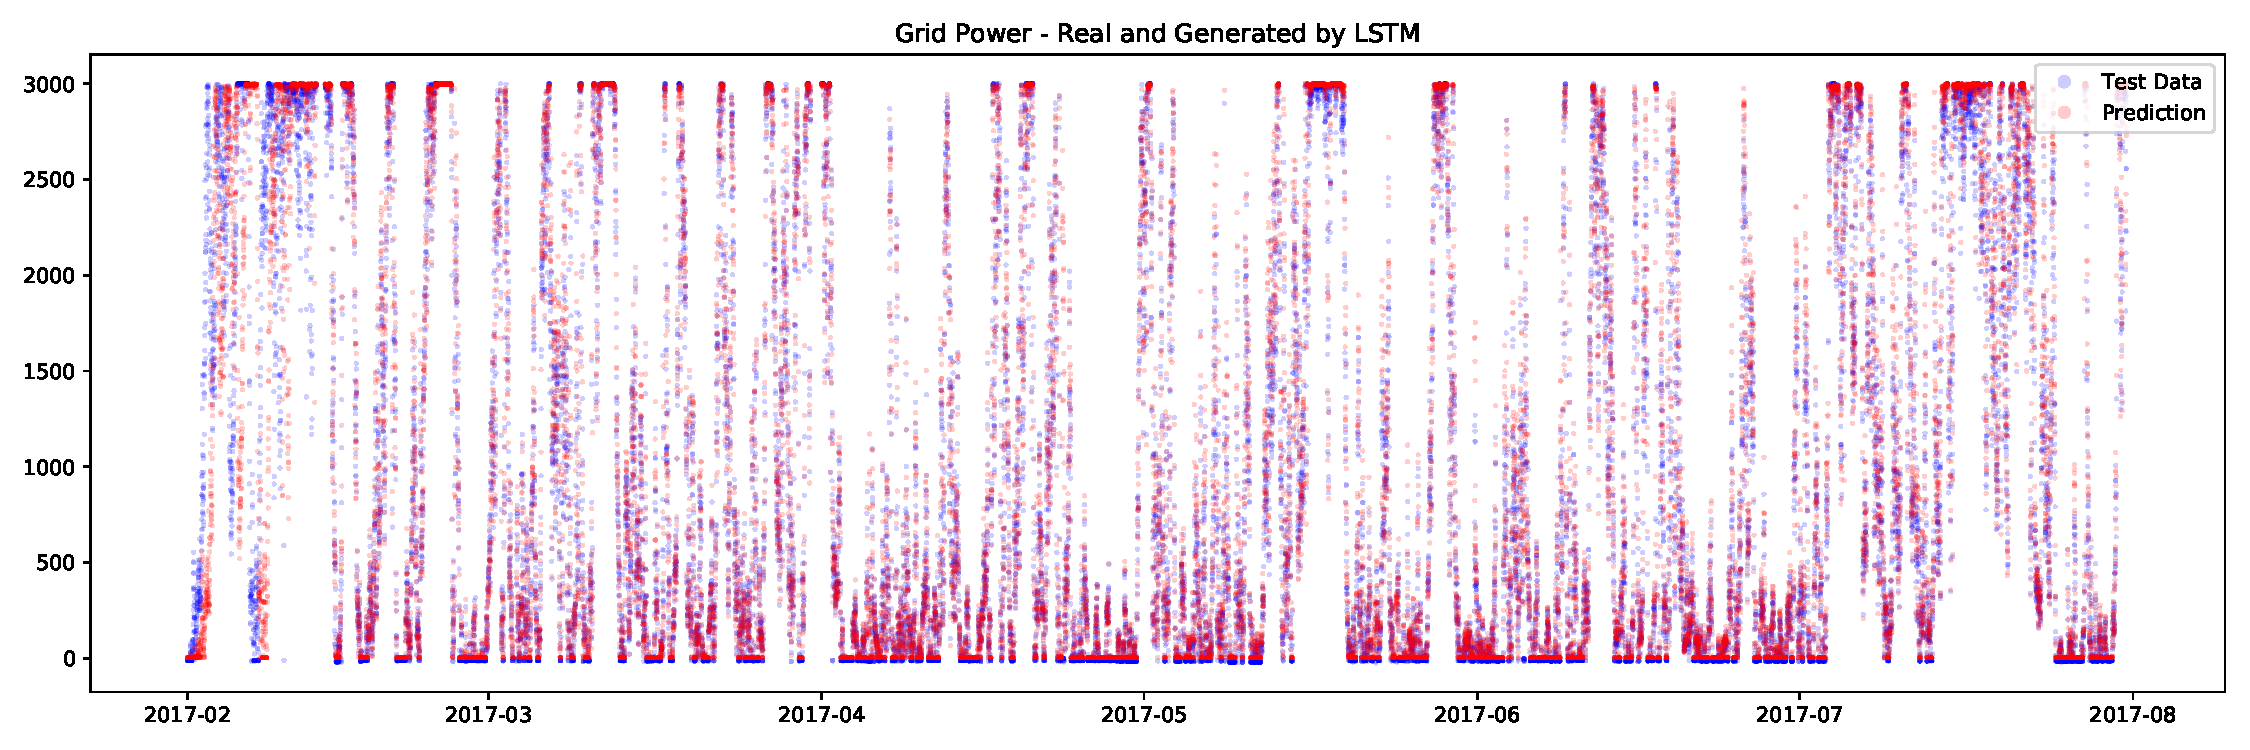
\includegraphics[width=0.9\textwidth]{lstm_grid_power_128_2_tukey.pdf}
        \label{fig:lstm_power}
    }
    
    \caption{Predicted generated power data for RNN and LSTM model with Tukey's biweight loss}
    \label{fig:deep_powers}
\end{figure}

\begin{figure}
    \centering
  \subfigure[RNN with MSE loss]{
       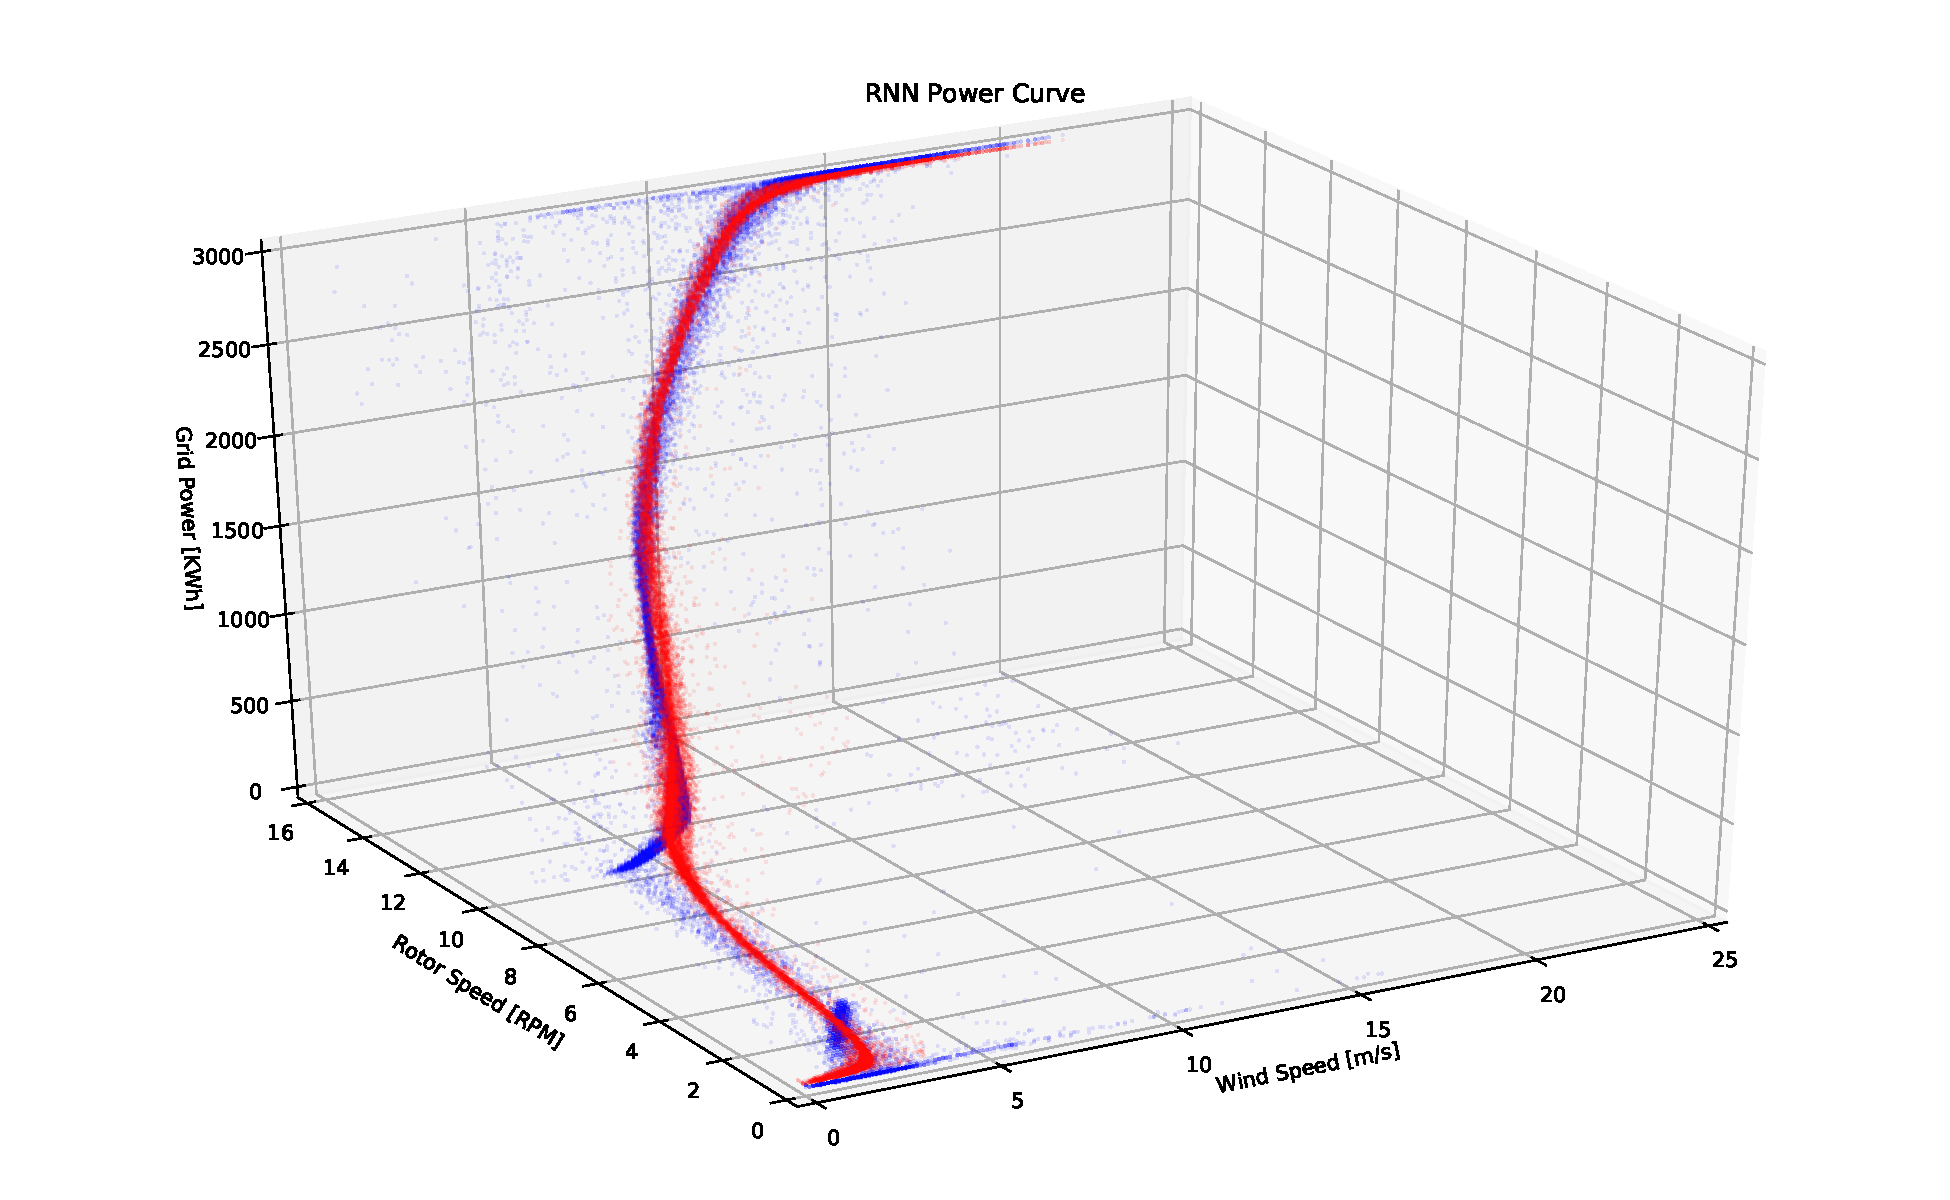
\includegraphics[width=0.47\textwidth]{rnn_power_curve_128_1_MSE.pdf}
       \label{fig:1-rnn-power_curve-figa}
    }%
  \hfill
  \subfigure[LSTM with MSE loss]{
       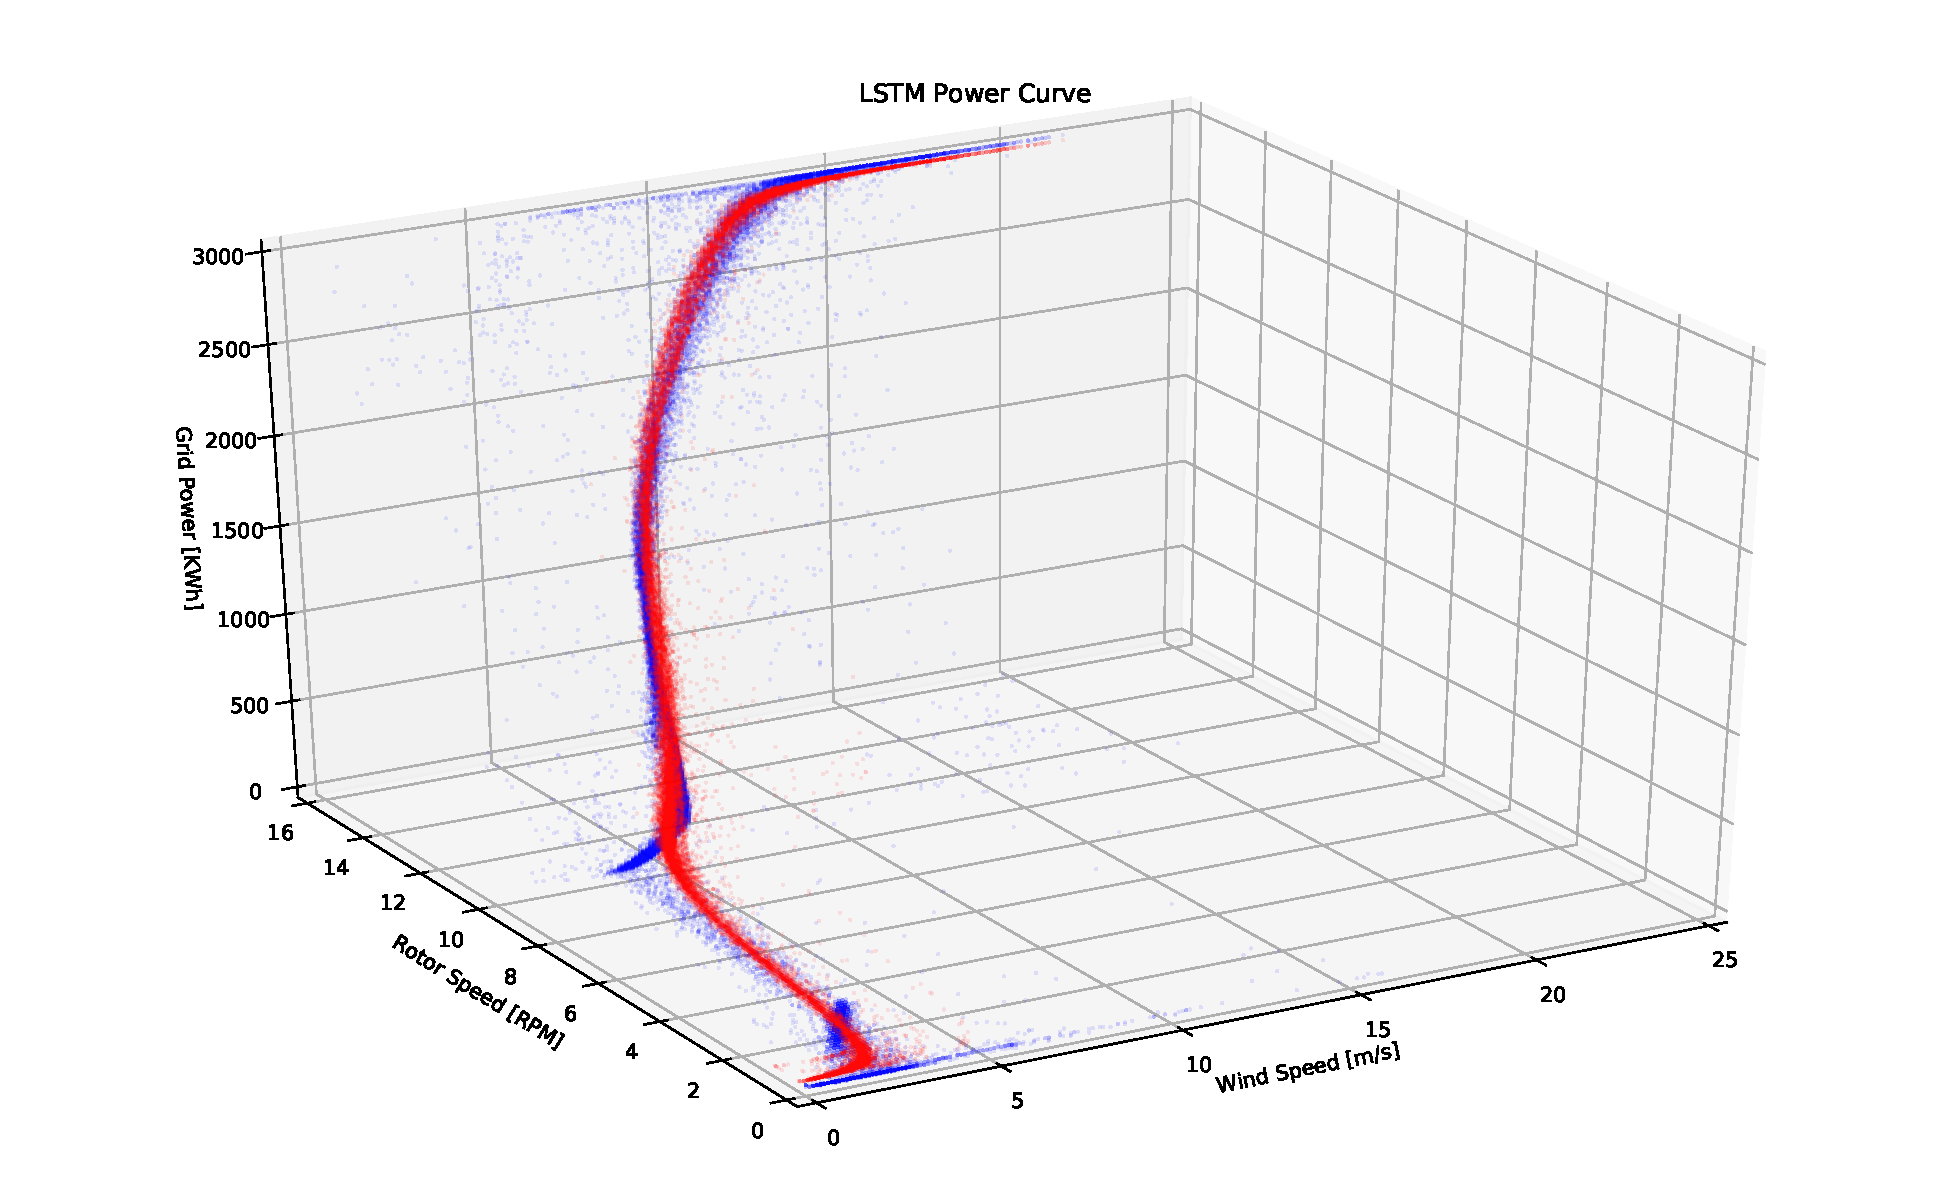
\includegraphics[width=0.47\textwidth]{lstm_power_curve_128_1_MSE.pdf}
       \label{fig:1-lstm-power_curve-figa}
  }
  
  \subfigure[RNN with L1 loss]{
       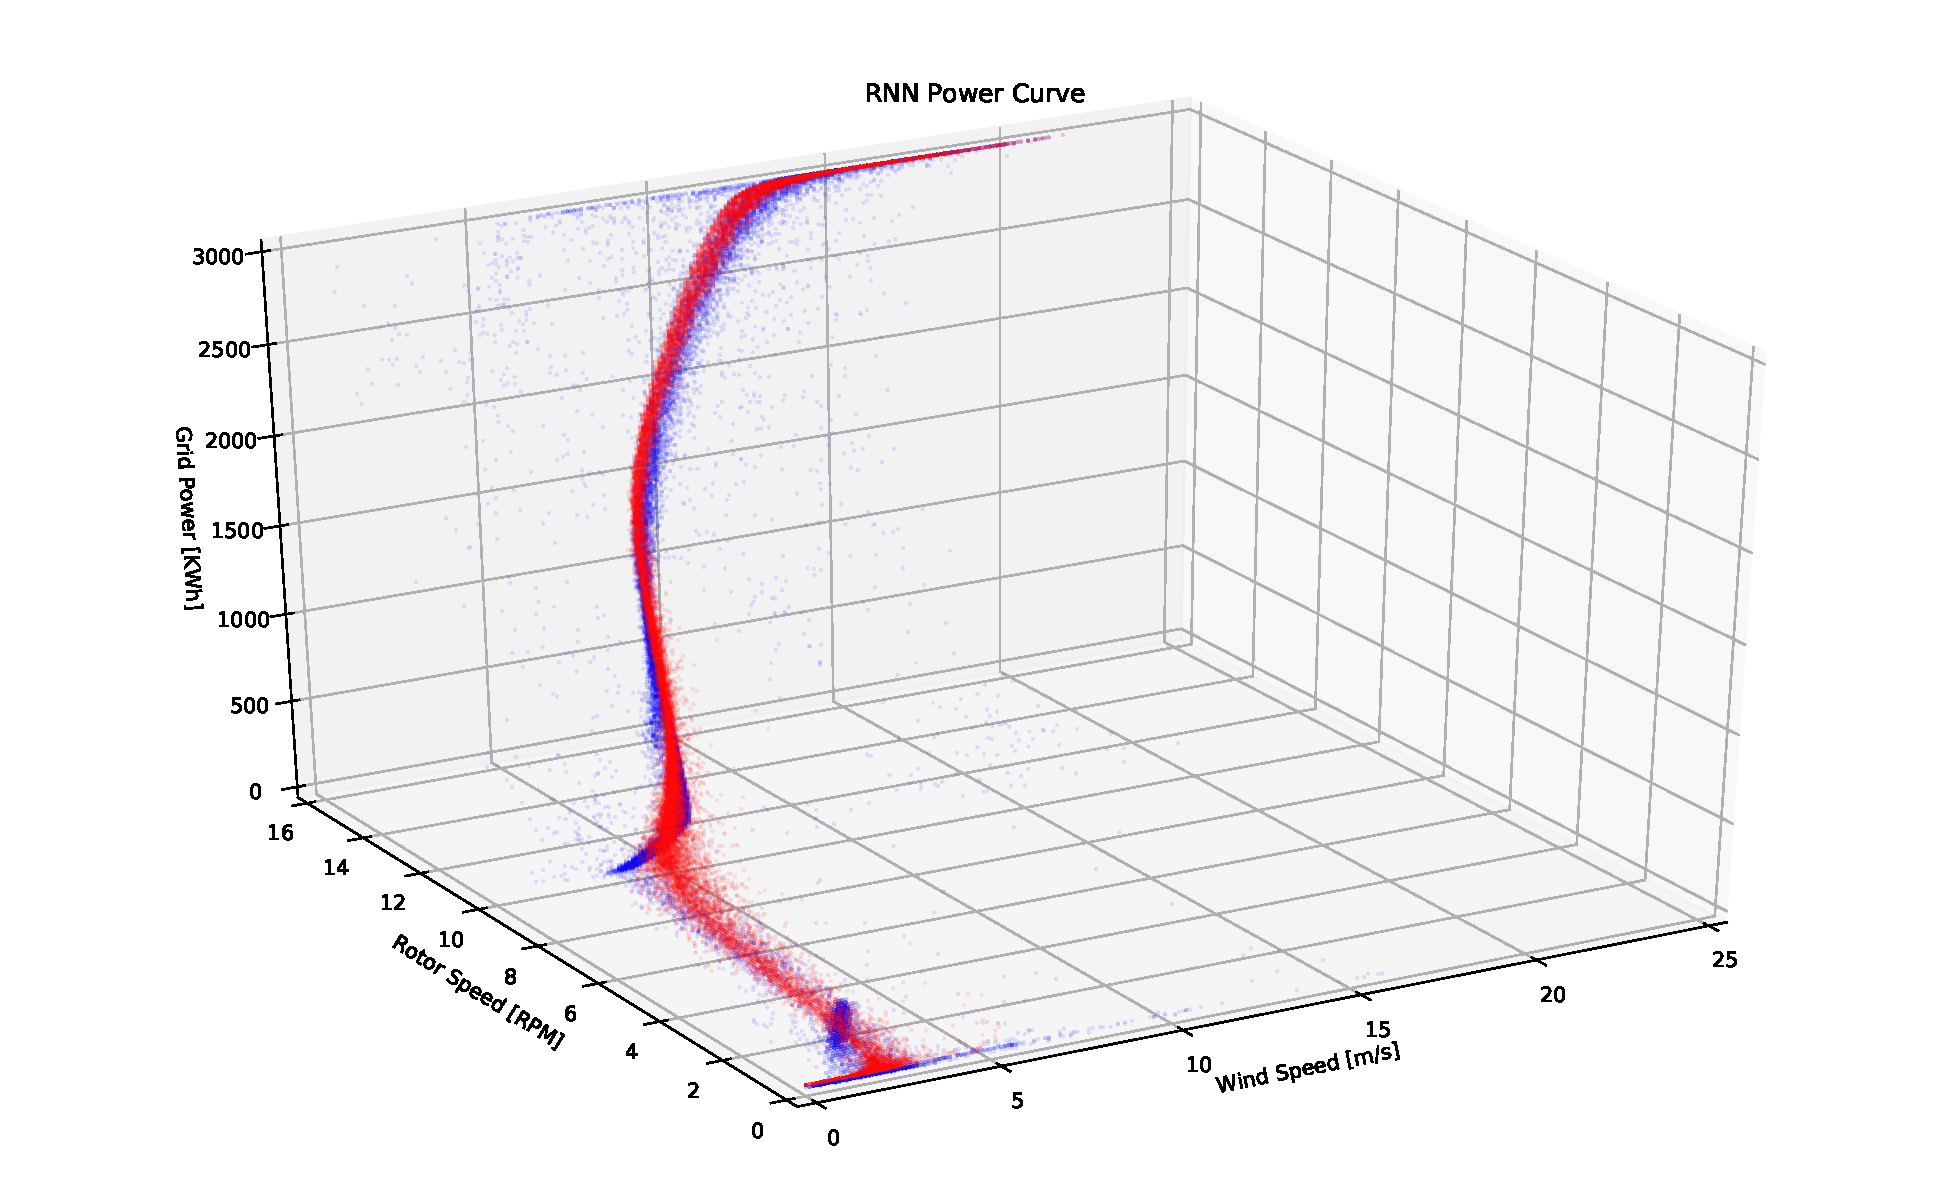
\includegraphics[width=0.47\textwidth]{rnn_power_curve_128_1_L1.pdf}
       \label{fig:1-rnn-power_curve-figb}
  }%
  \hfill
  \subfigure[LSTM with L1 loss]{
       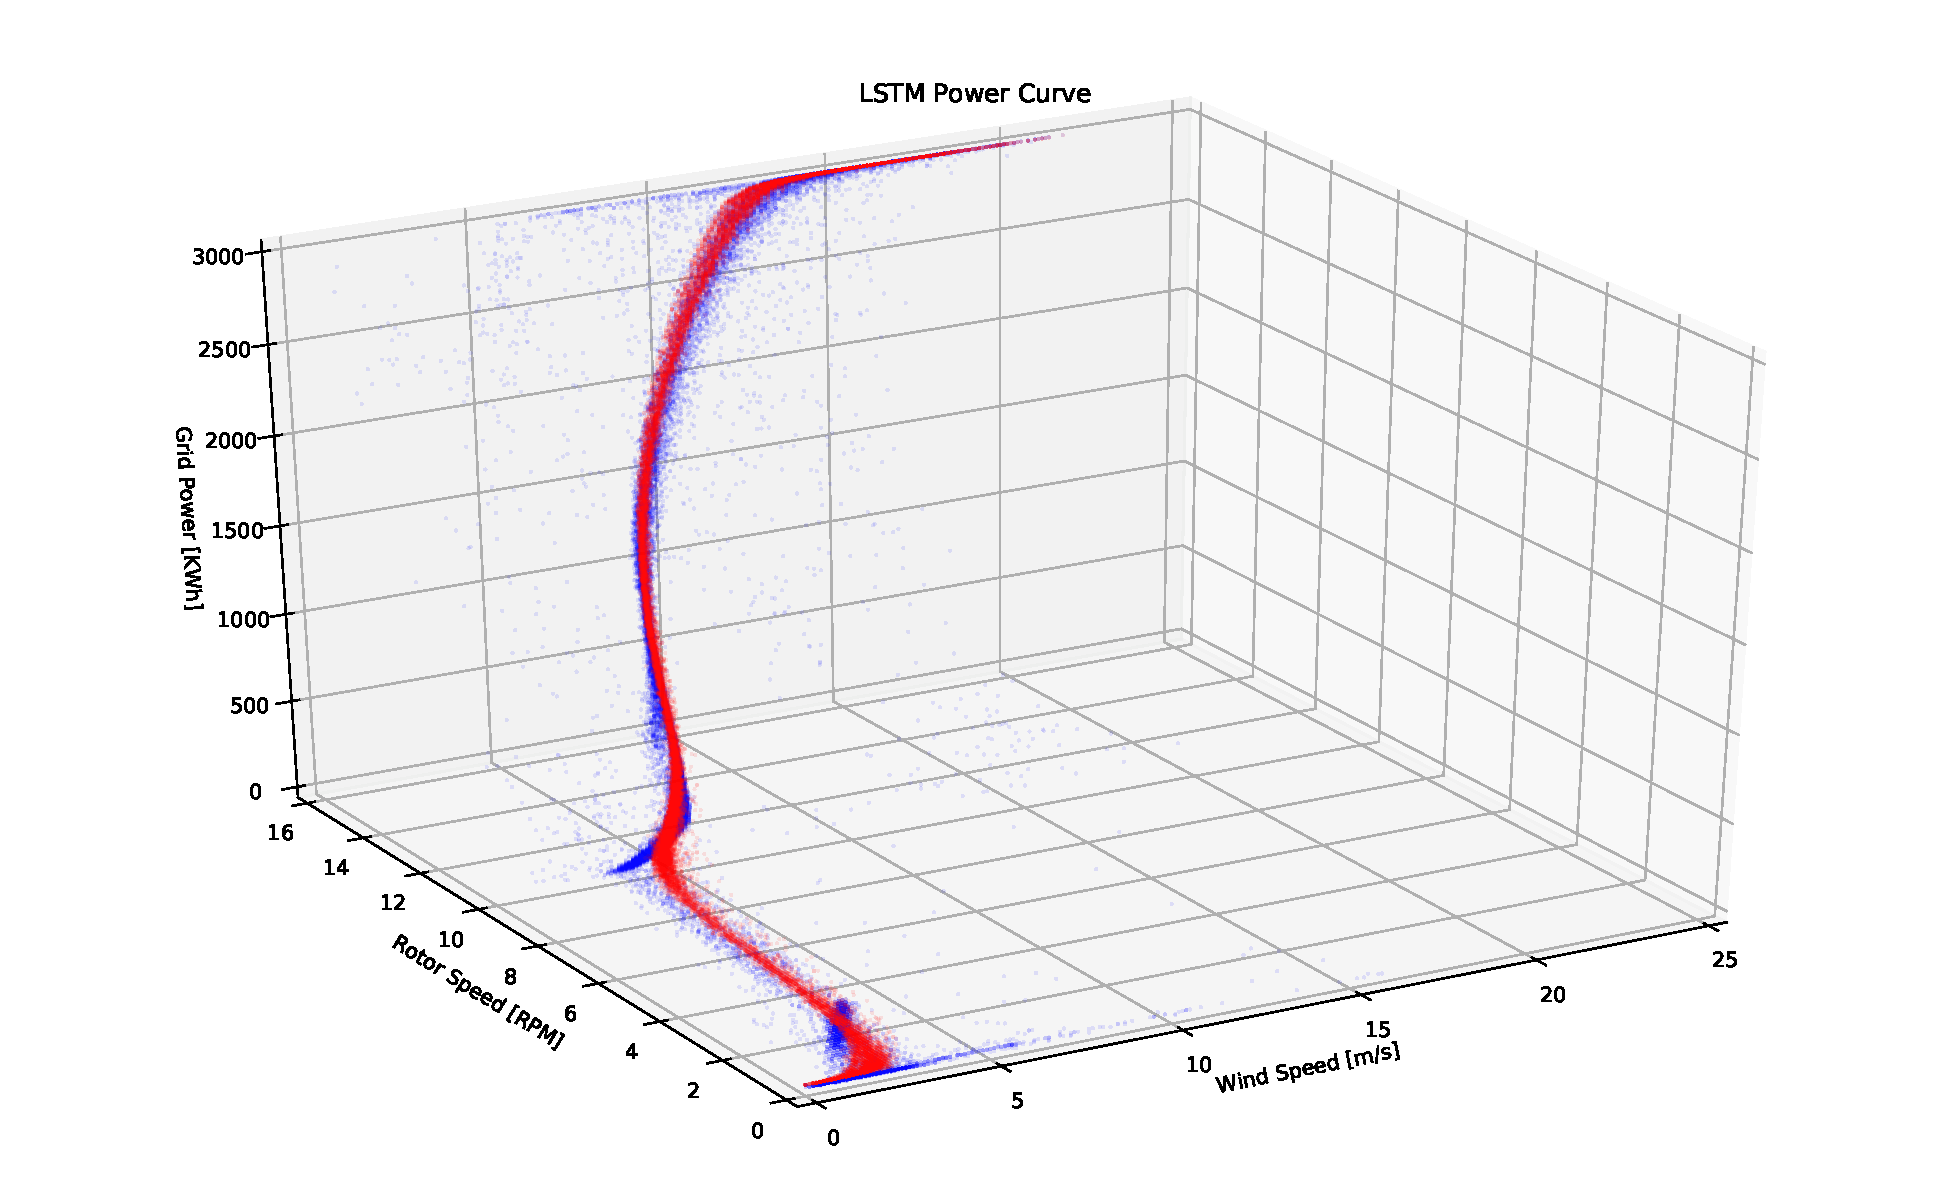
\includegraphics[width=0.47\textwidth]{lstm_power_curve_128_1_L1.pdf}
        \label{fig:1-lstm-power_curve-figb}
  }
  
  \subfigure[RNN with Tukey's biweight loss]{
       %\centering
       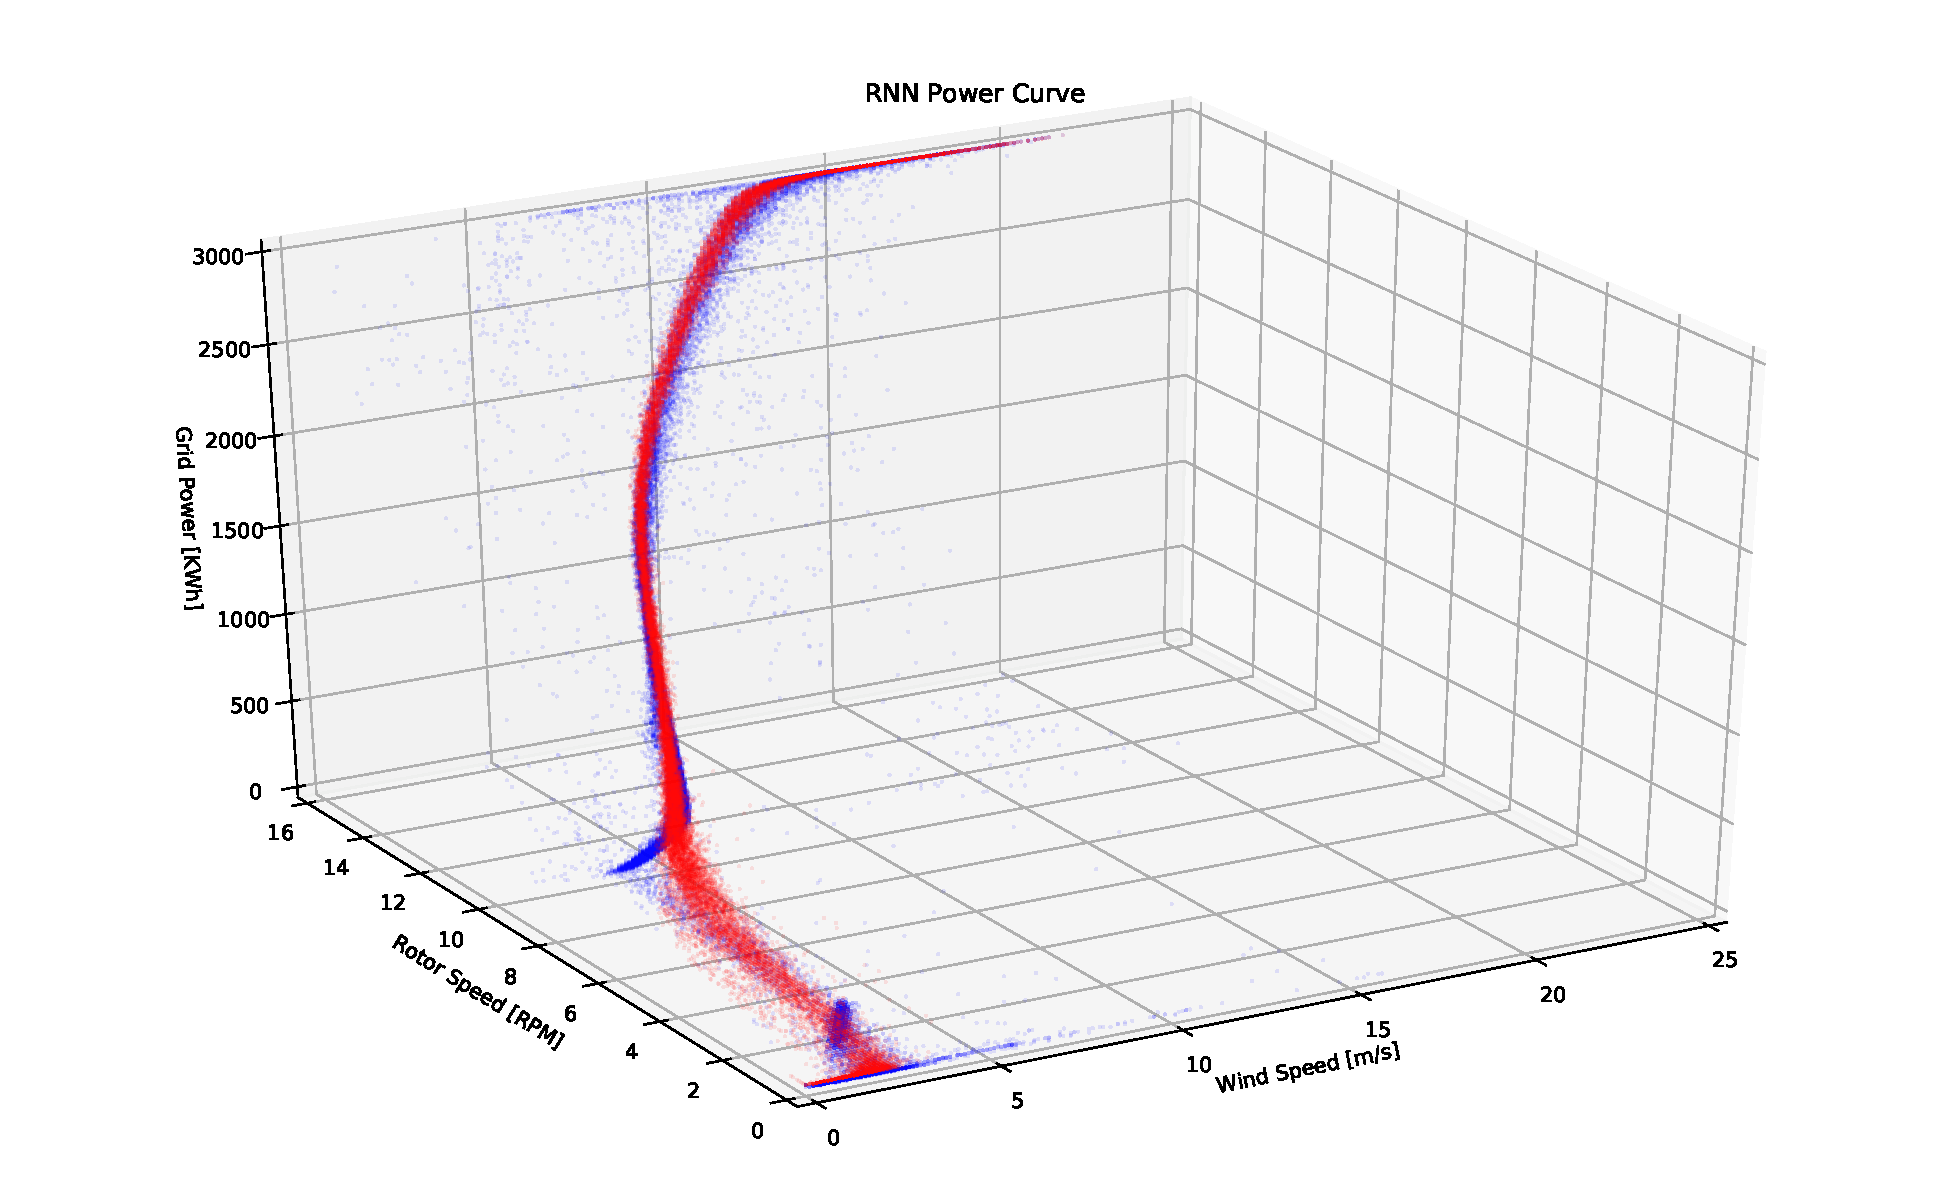
\includegraphics[width=0.47\textwidth]{rnn_power_curve_128_1_tukey.pdf}
        \label{fig:1-rnn-power_curve-figc}
  }%
  \hfill
  \subfigure[LSTM with Tukey's biweight loss]{
       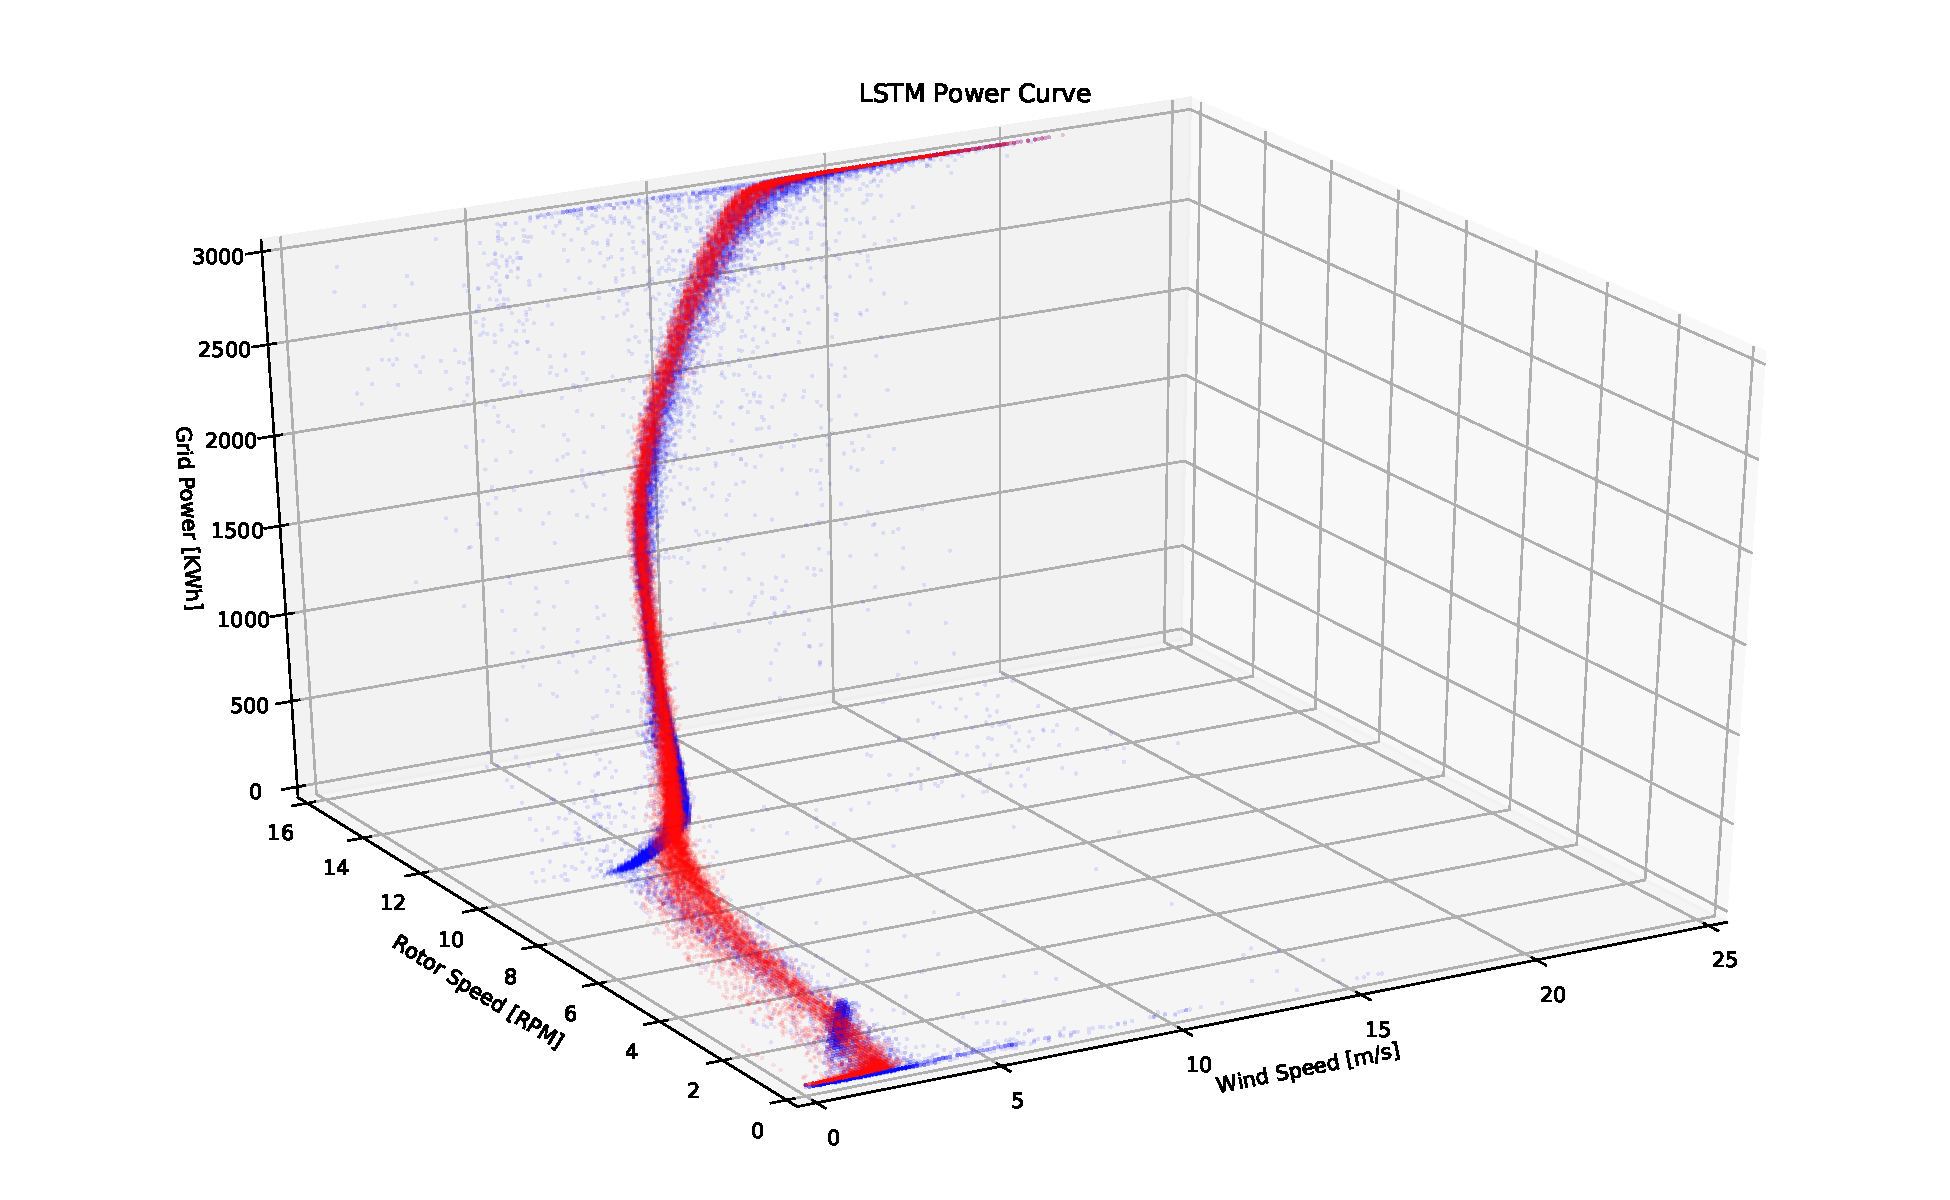
\includegraphics[width=0.47\textwidth]{lstm_power_curve_128_1_tukey.pdf}
       \label{fig:1-lstm-power_curve-figc}
  }
  \vspace{10pt}
  \caption{Generated from 1-layer network and observed power curves}
  \label{fig:1-deep_power_curves}
\end{figure}

\begin{figure}
    \centering
  \subfigure[RNN with MSE loss]{
       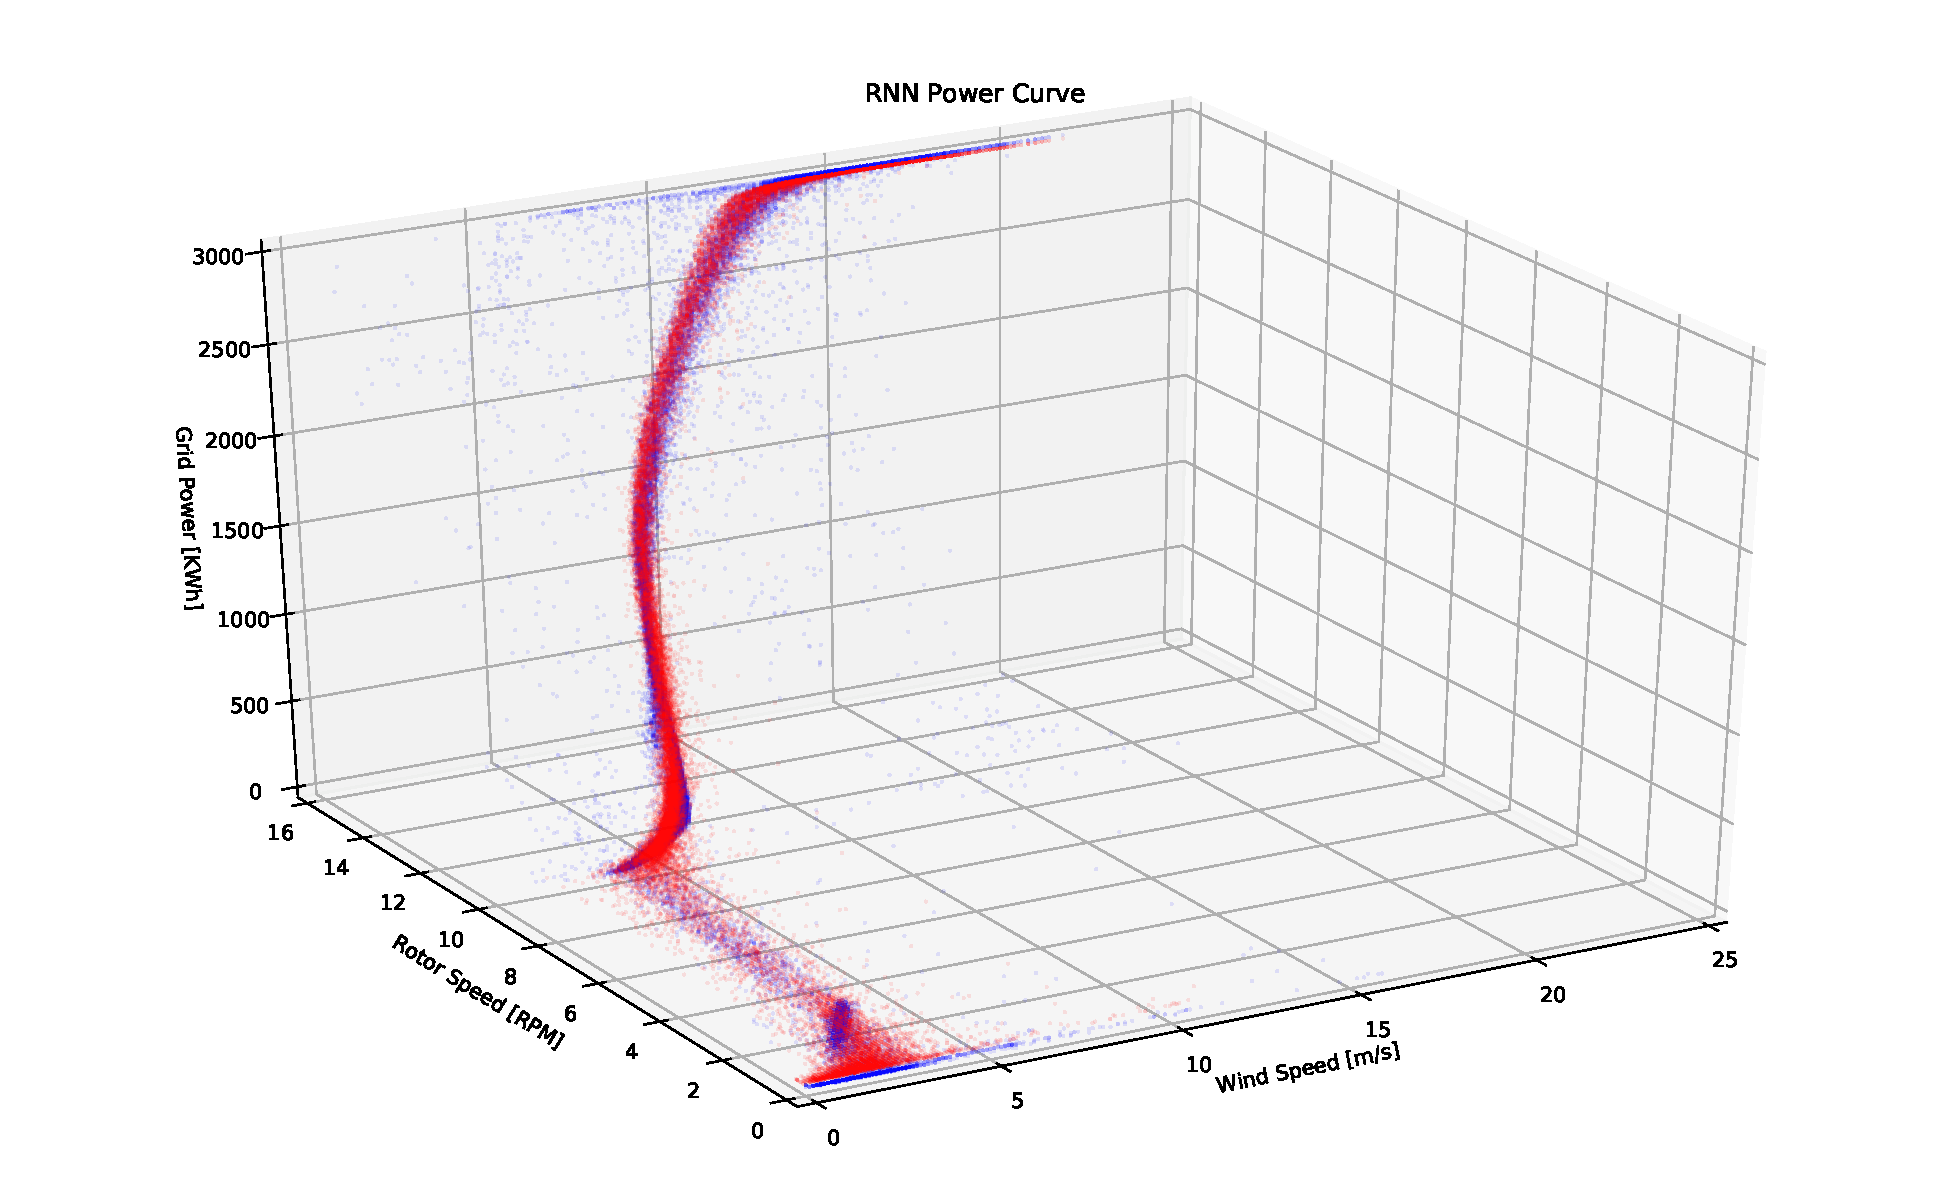
\includegraphics[width=0.47\textwidth]{rnn_power_curve_128_2_MSE.pdf}
       \label{fig:2-rnn-power_curve-figa}
    }%
  \hfill
  \subfigure[LSTM with MSE loss]{
       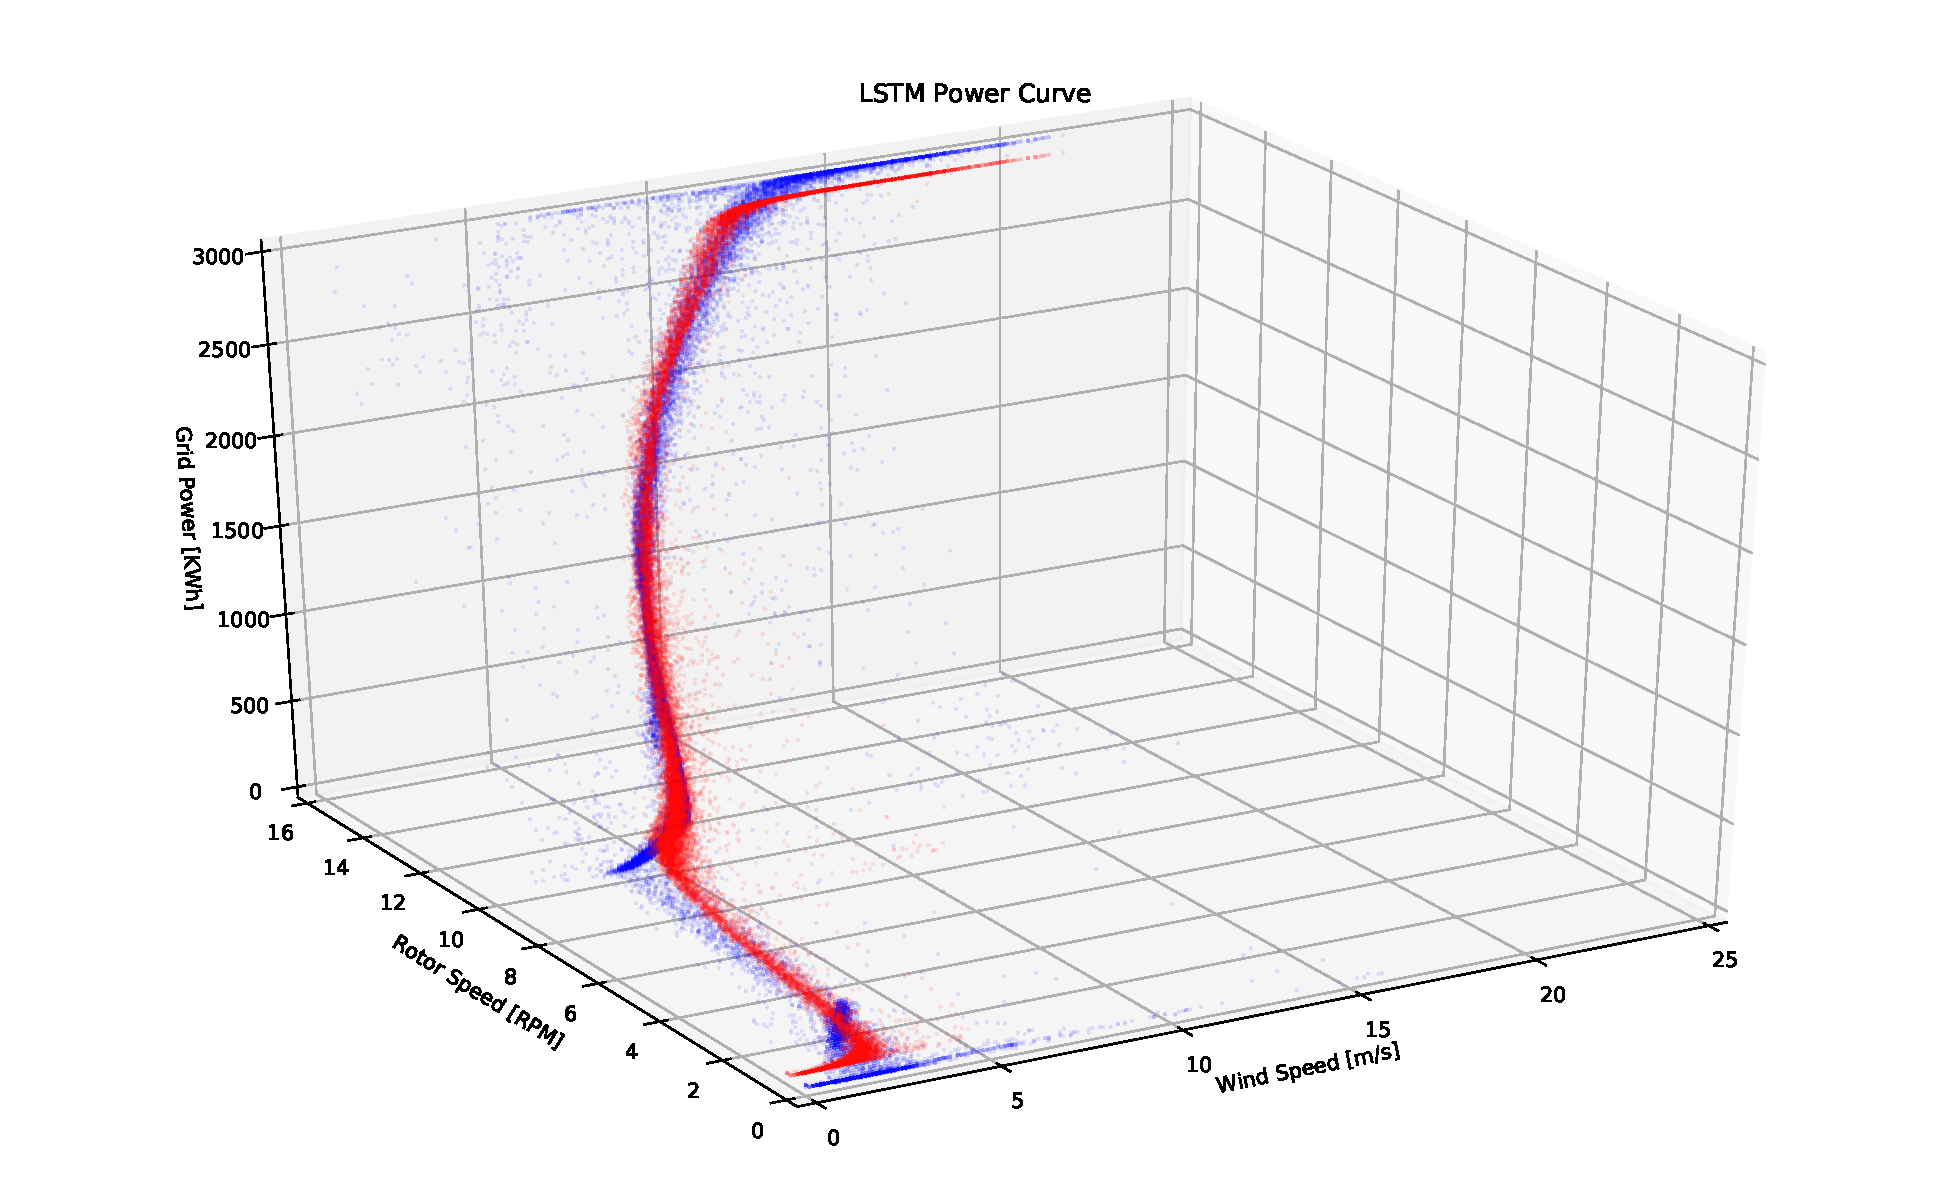
\includegraphics[width=0.47\textwidth]{lstm_power_curve_128_2_MSE.pdf}
       \label{fig:2-lstm-power_curve-figa}
  }
  
  \subfigure[RNN with L1 loss]{
       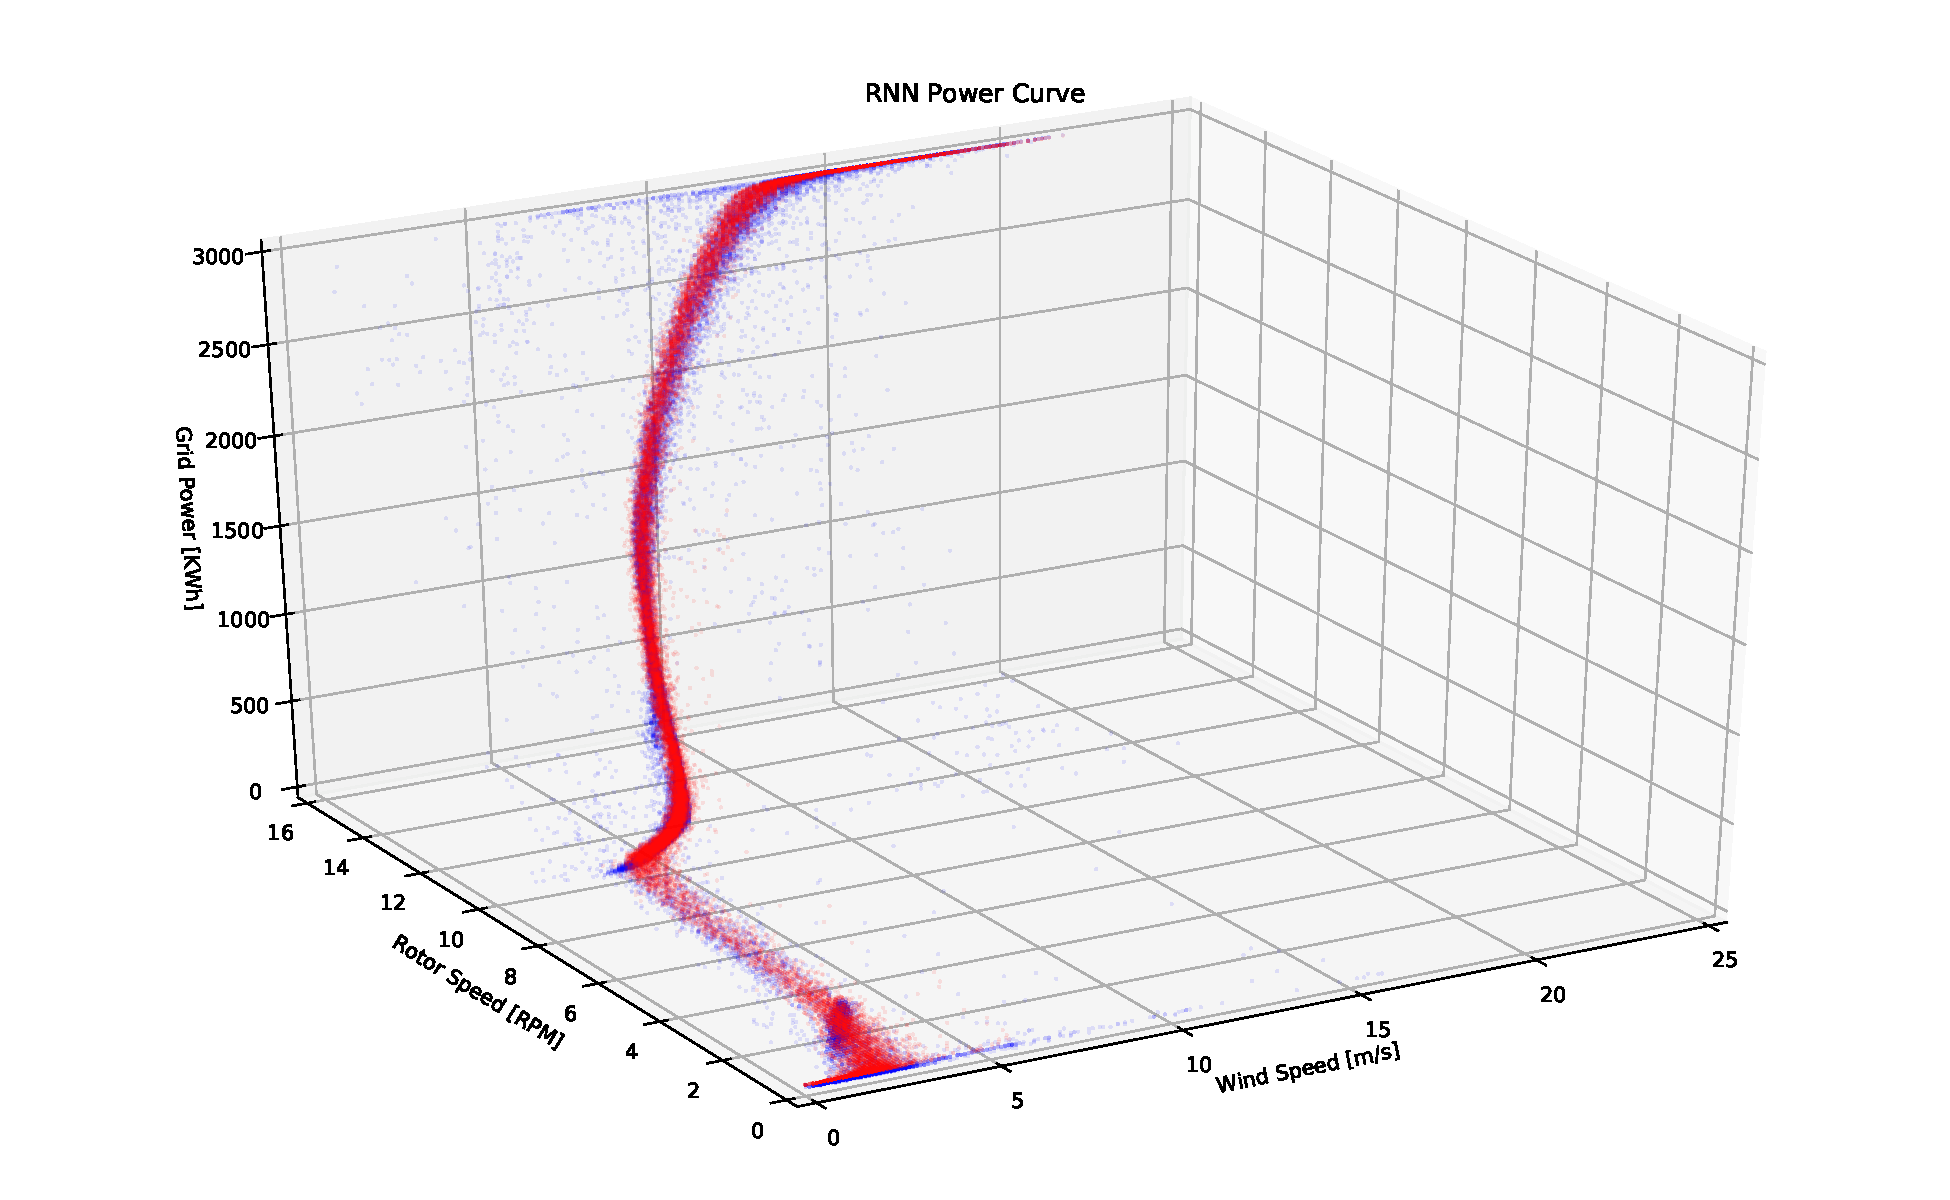
\includegraphics[width=0.47\textwidth]{rnn_power_curve_128_2_L1.pdf}
       \label{fig:2-rnn-power_curve-figb}
  }%
  \hfill
  \subfigure[LSTM with L1 loss]{
       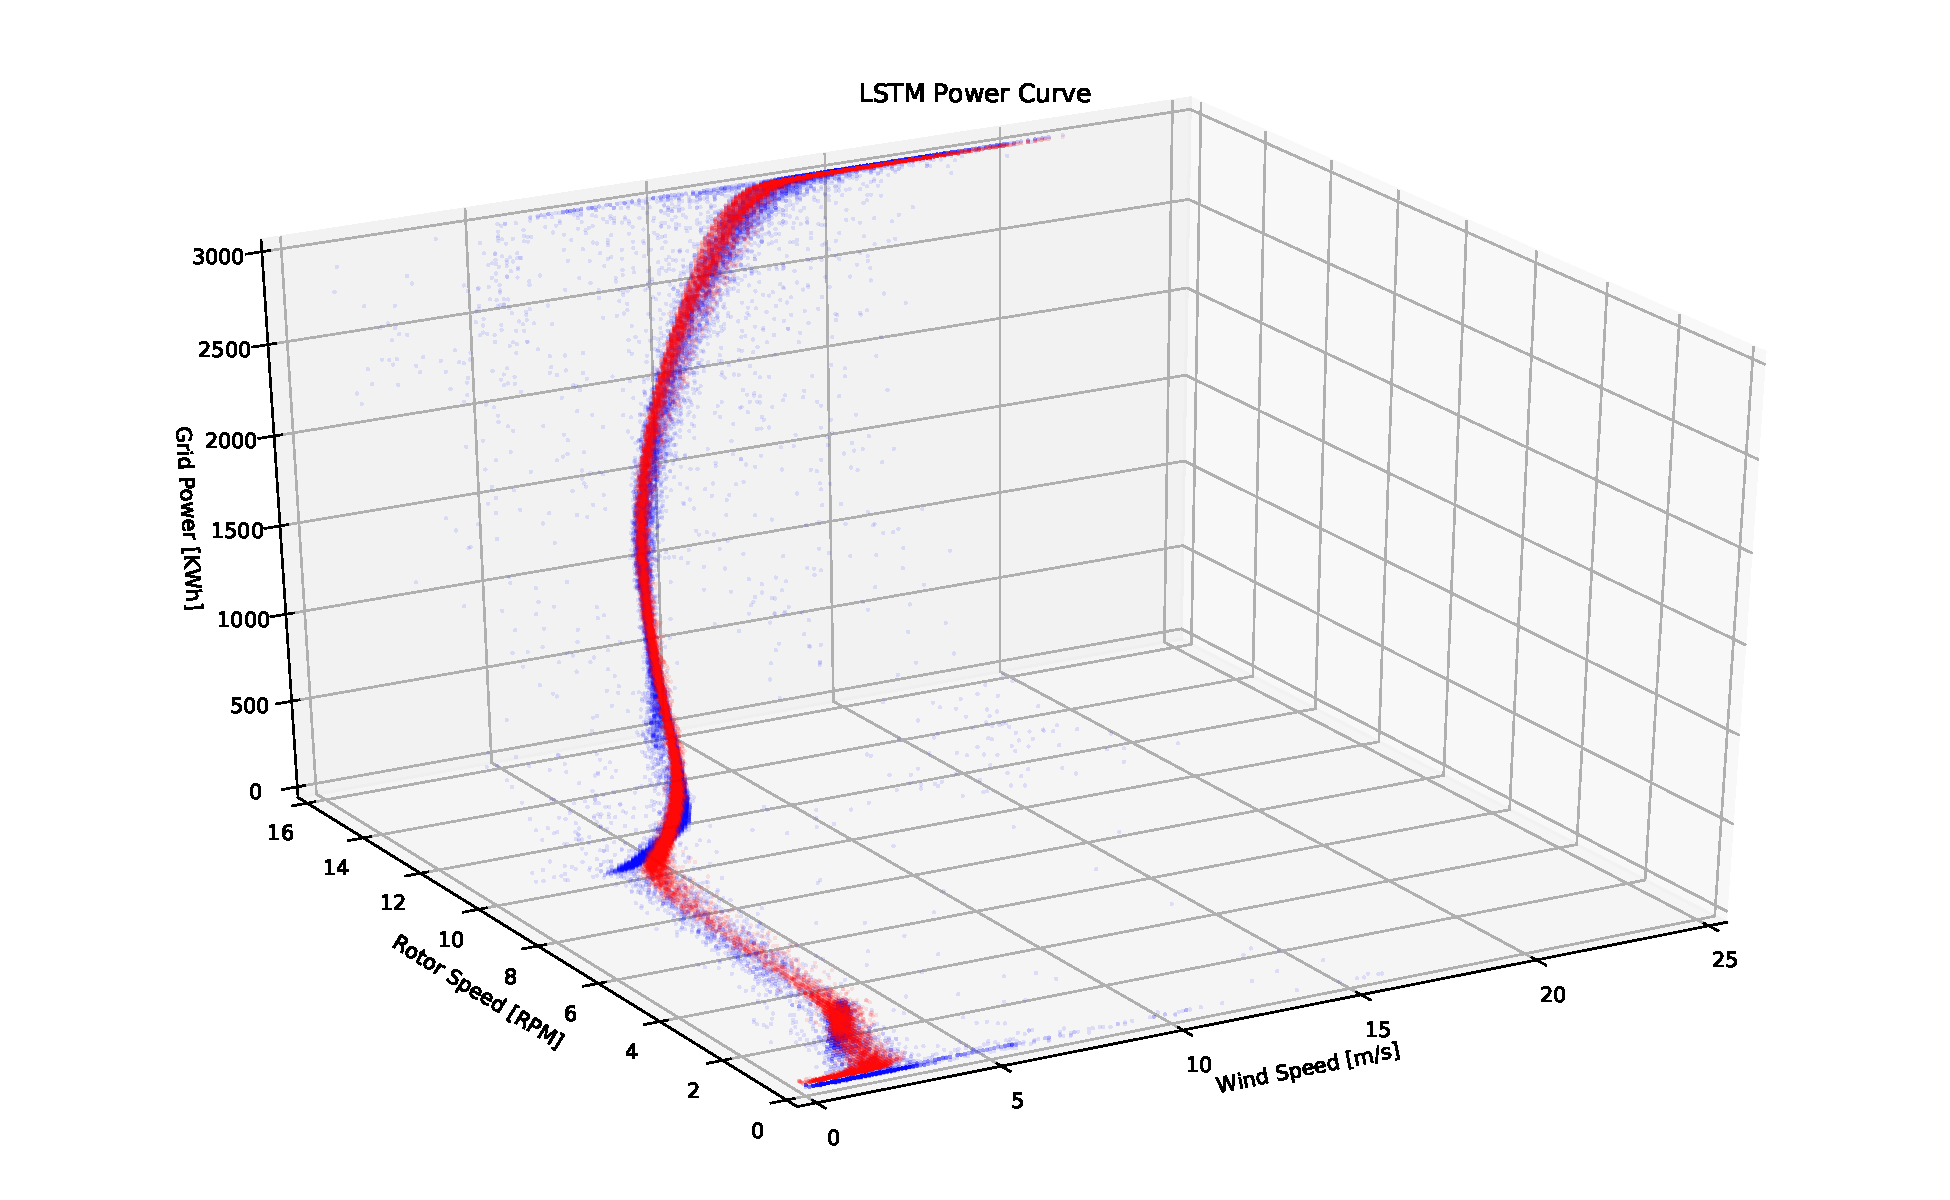
\includegraphics[width=0.47\textwidth]{lstm_power_curve_128_2_L1.pdf}
        \label{fig:2-lstm-power_curve-figb}
  }
  
  \subfigure[RNN with Tukey's biweight loss]{
       %\centering
       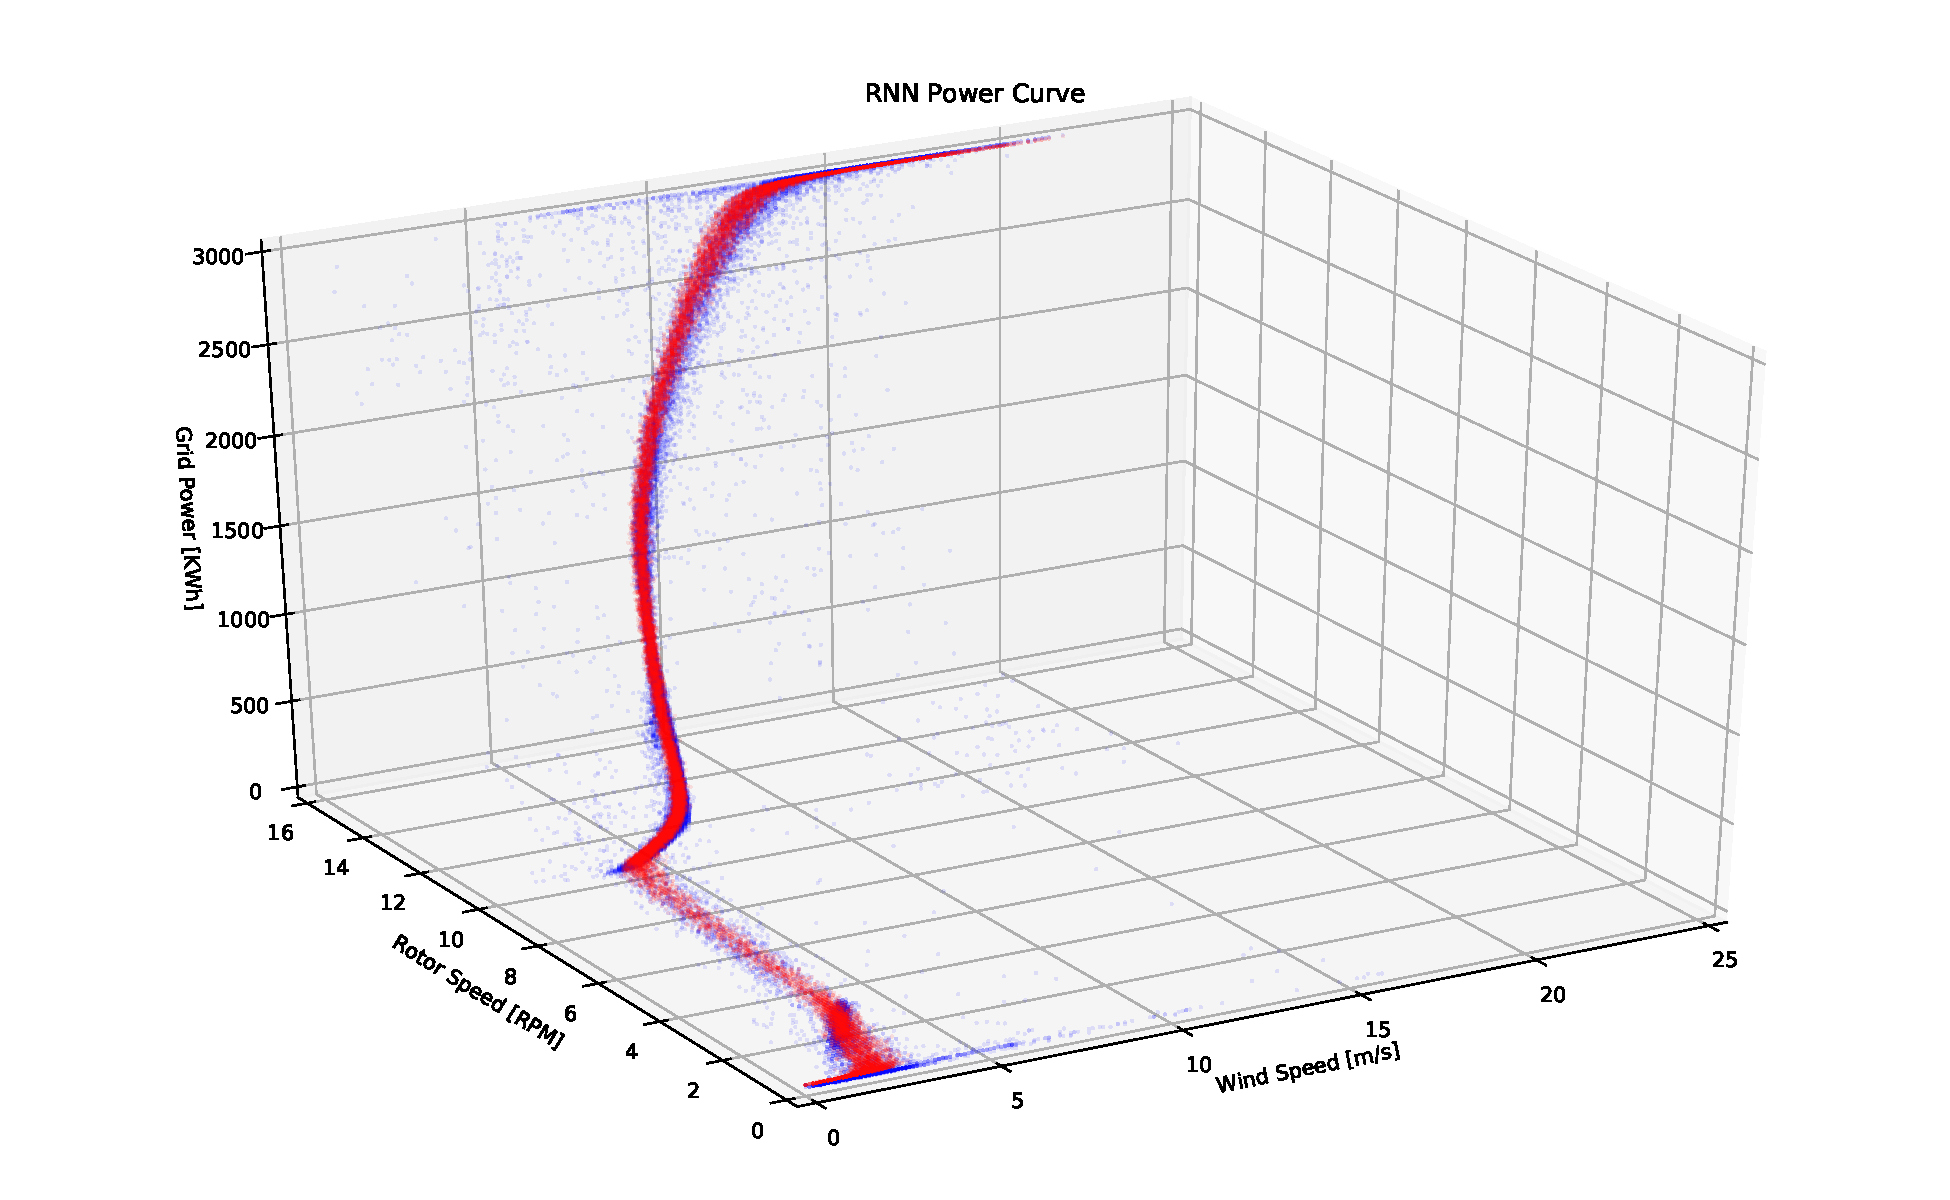
\includegraphics[width=0.47\textwidth]{rnn_power_curve_128_2_tukey.pdf}
        \label{fig:2-rnn-power_curve-figc}
  }%
  \hfill
  \subfigure[LSTM with Tukey's biweight loss]{
       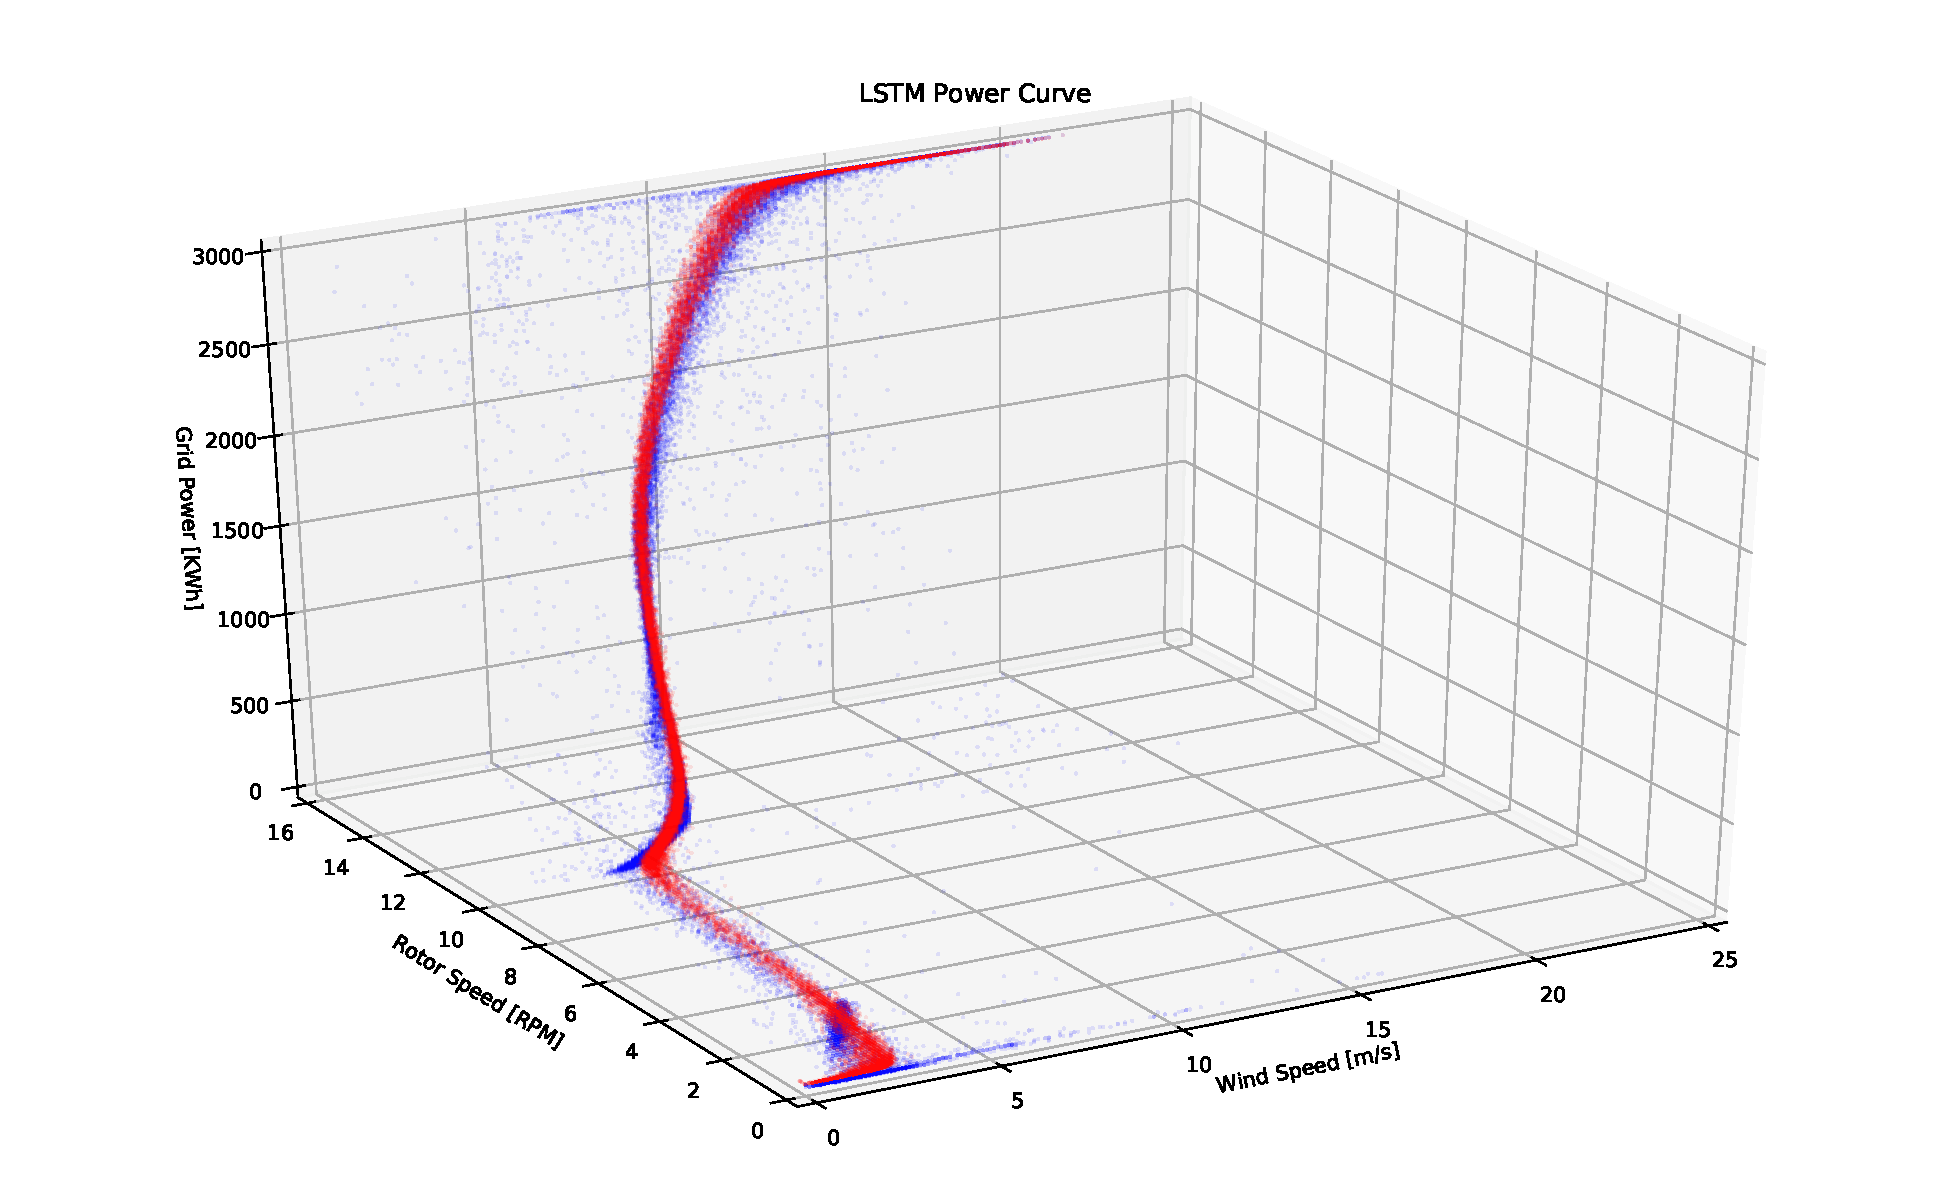
\includegraphics[width=0.47\textwidth]{lstm_power_curve_128_2_tukey.pdf}
       \label{fig:2-lstm-power_curve-figc}
  }
  \vspace{10pt}
  \caption{Generated from 2-layer network and observed power curves}
  \label{fig:2-deep_power_curves}
\end{figure}



\begin{figure}
    \centering
  \subfigure[RNN with MSE loss]{
       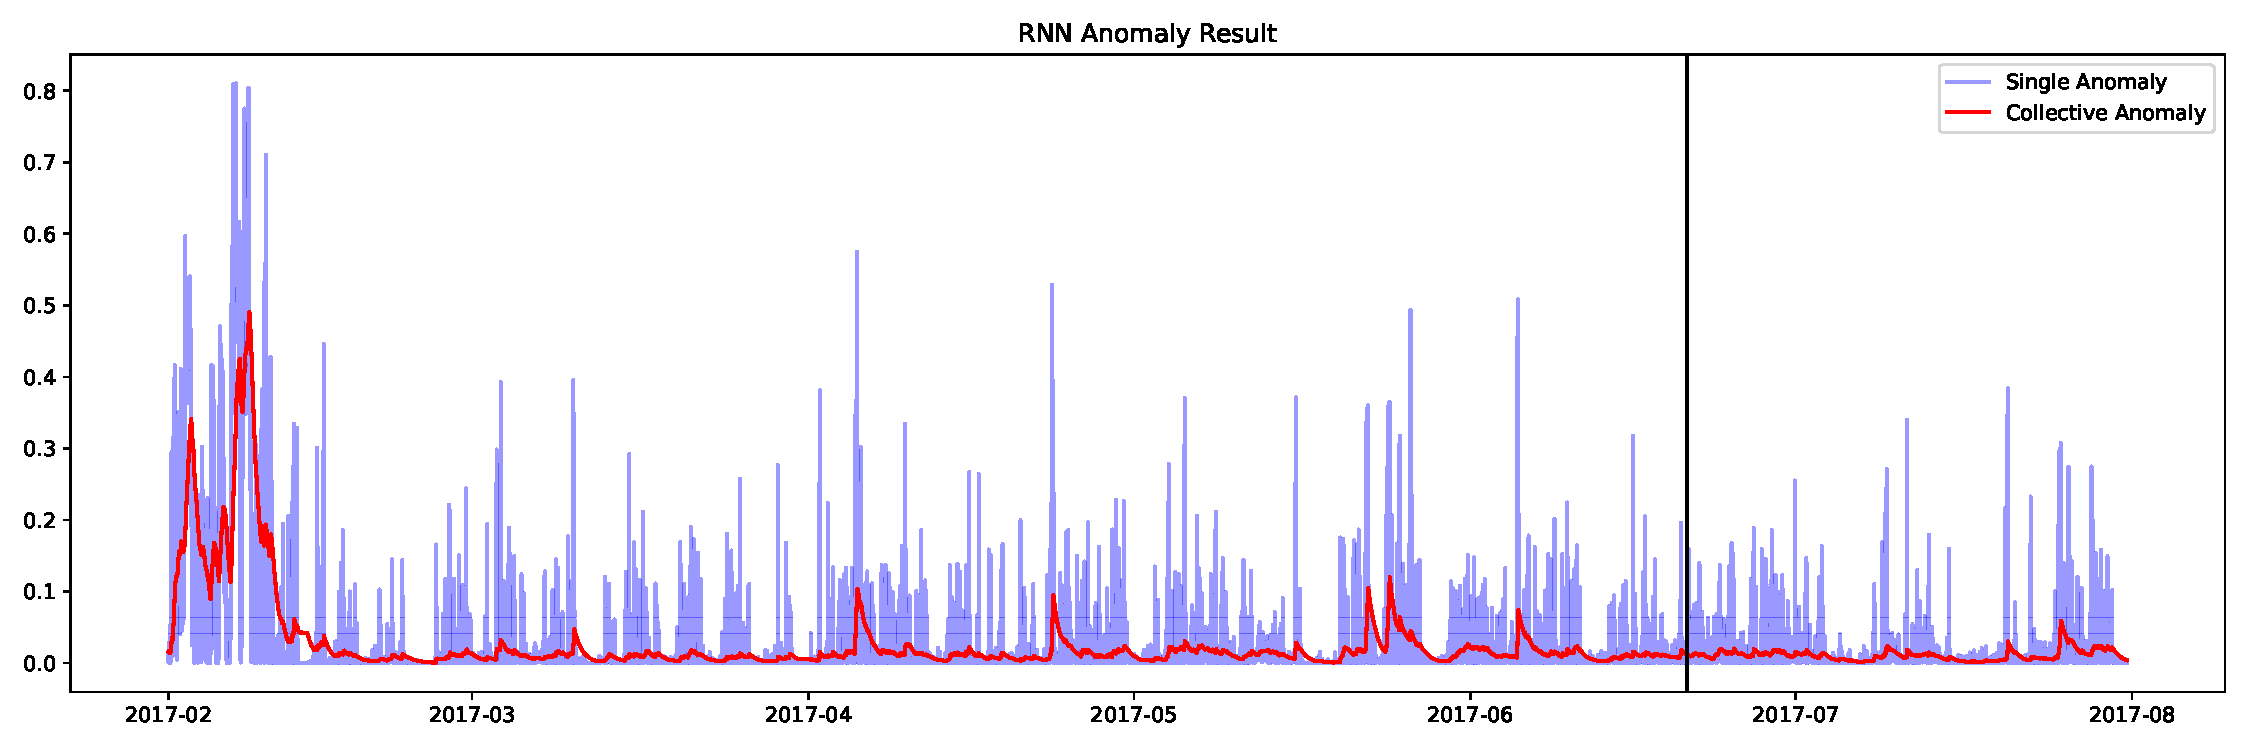
\includegraphics[width=0.48\textwidth]{rnn_anomaly_128_1_MSE.pdf}
       \label{fig:1-rnn-anomaly-figa}
    }%
  \hfill
  \subfigure[LSTM with MSE loss]{
       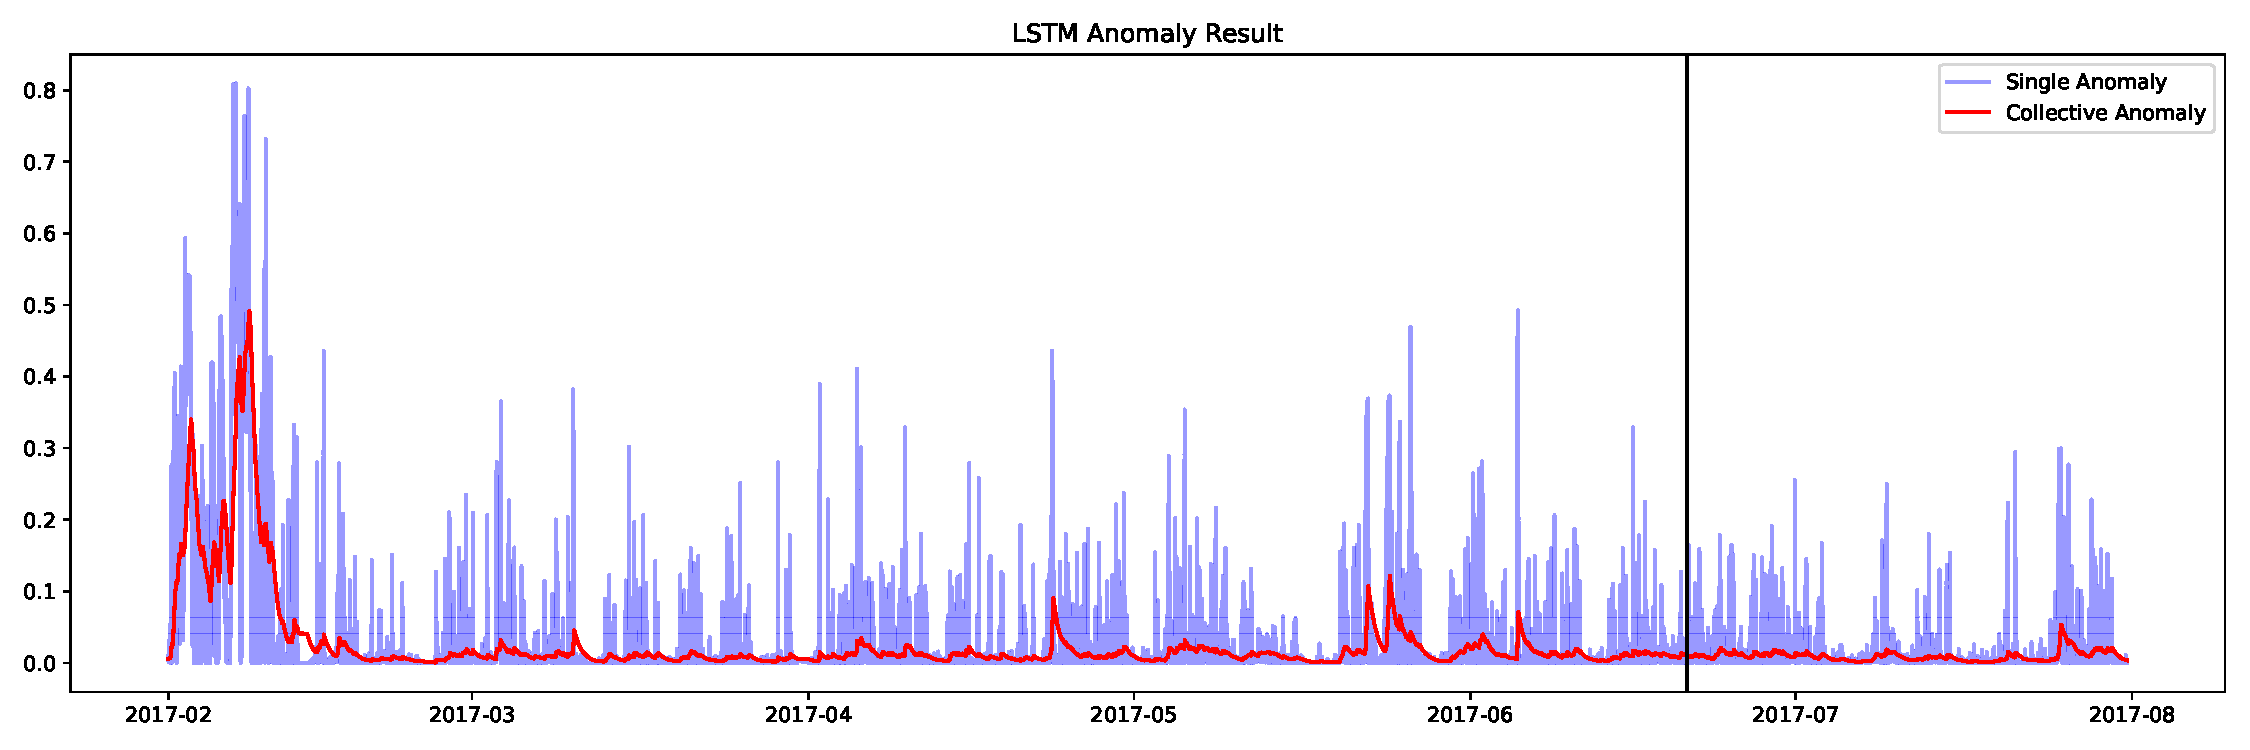
\includegraphics[width=0.48\textwidth]{lstm_anomaly_128_1_MSE.pdf}
       \label{fig:1-lstm-anomaly-figa}
  }
  
  \subfigure[RNN with L1 loss]{
       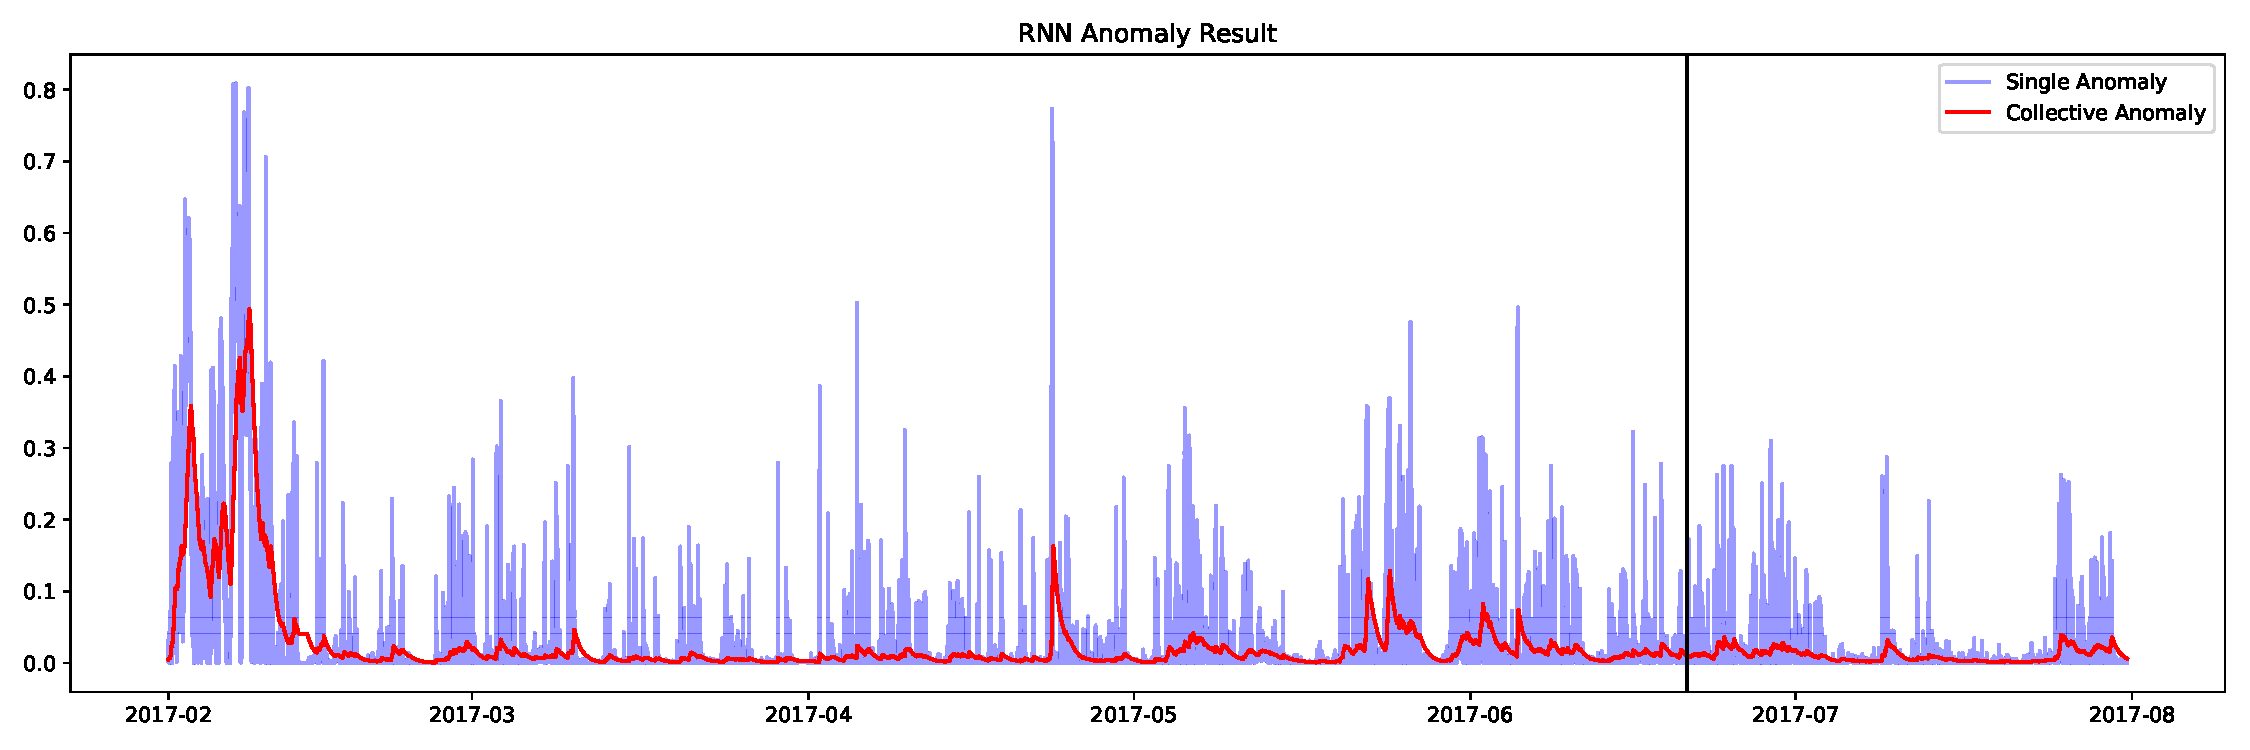
\includegraphics[width=0.48\textwidth]{rnn_anomaly_128_1_L1.pdf}
       \label{fig:1-rnn-anomaly-figb}
  }%
  \hfill
  \subfigure[LSTM with L1 loss]{
       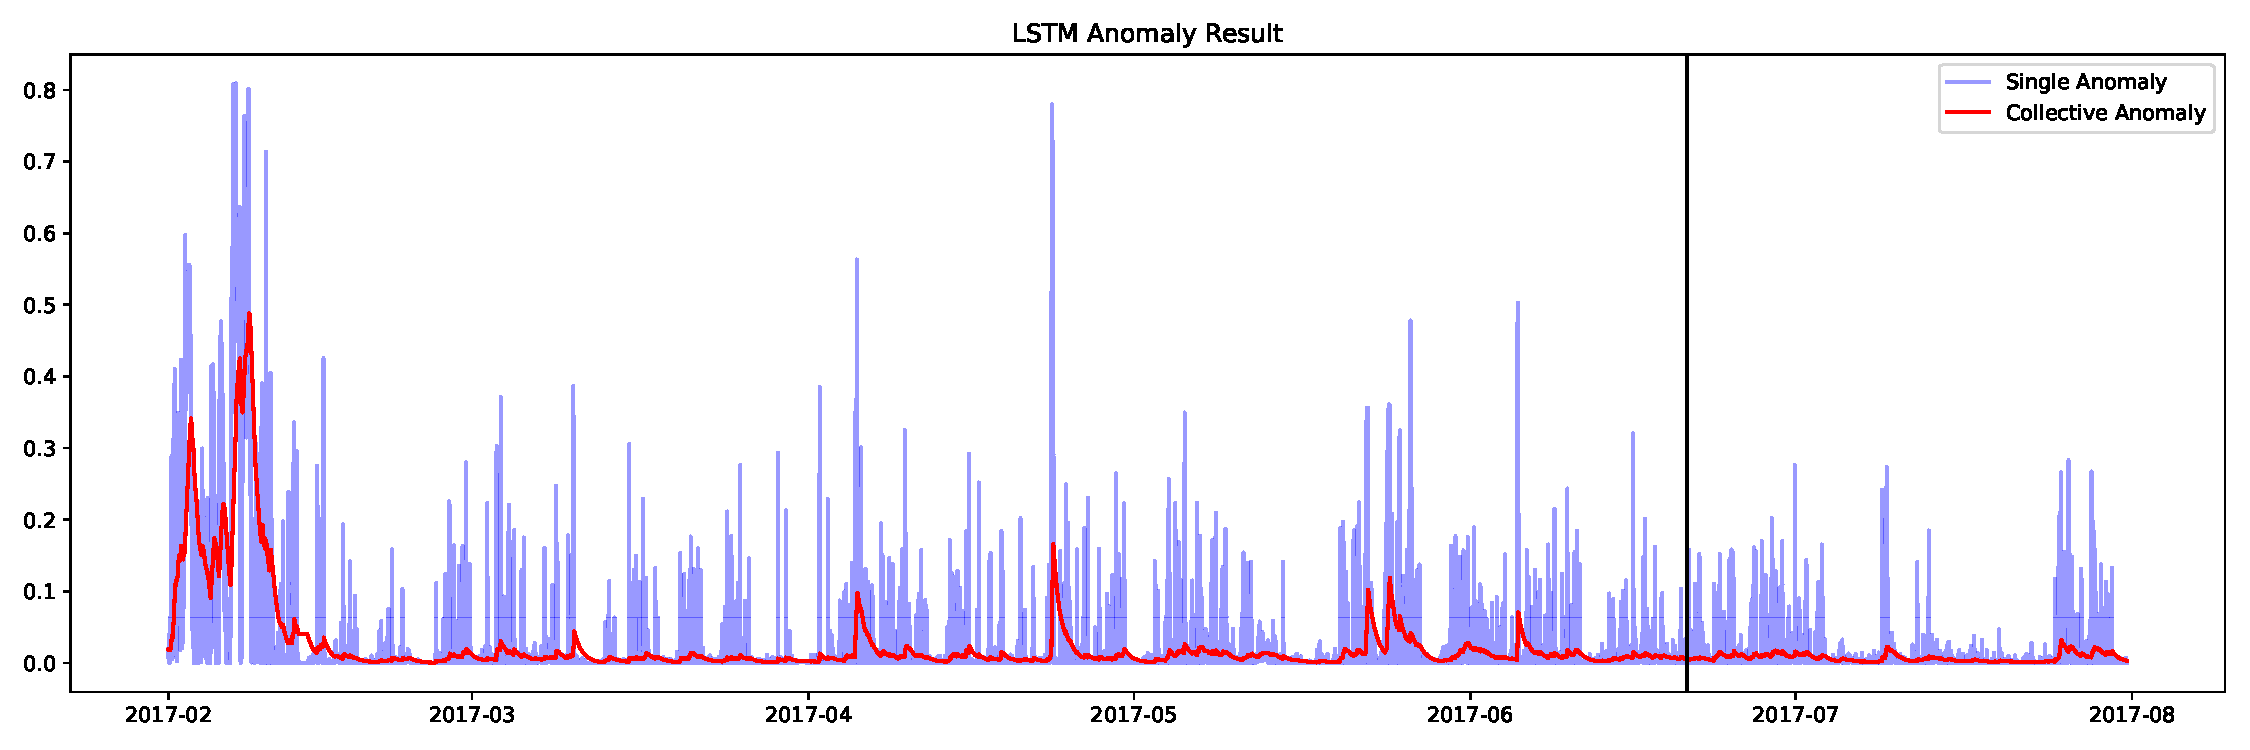
\includegraphics[width=0.48\textwidth]{lstm_anomaly_128_1_L1.pdf}
        \label{fig:1-lstm-anomaly-figb}
  }
  
  \subfigure[RNN with Tukey's biweight loss]{
       %\centering
       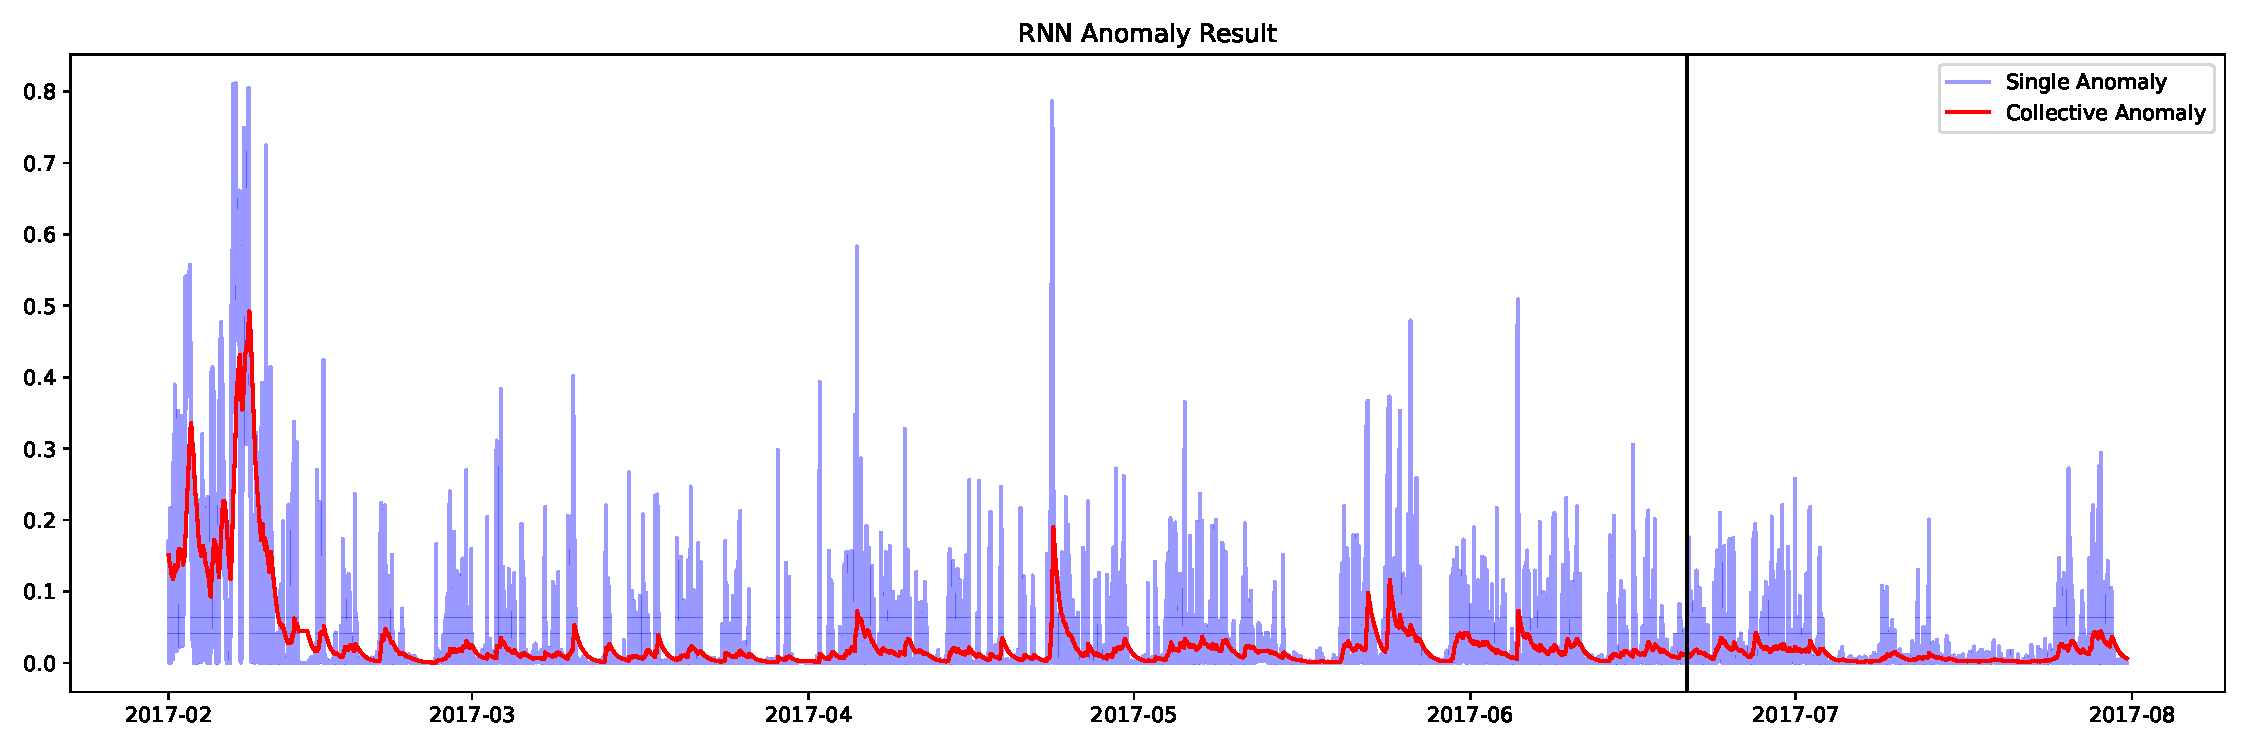
\includegraphics[width=0.48\textwidth]{rnn_anomaly_128_1_tukey.pdf}
        \label{fig:1-rnn-anomaly-figc}
  }%
  \hfill
  \subfigure[LSTM with Tukey's biweight loss]{
       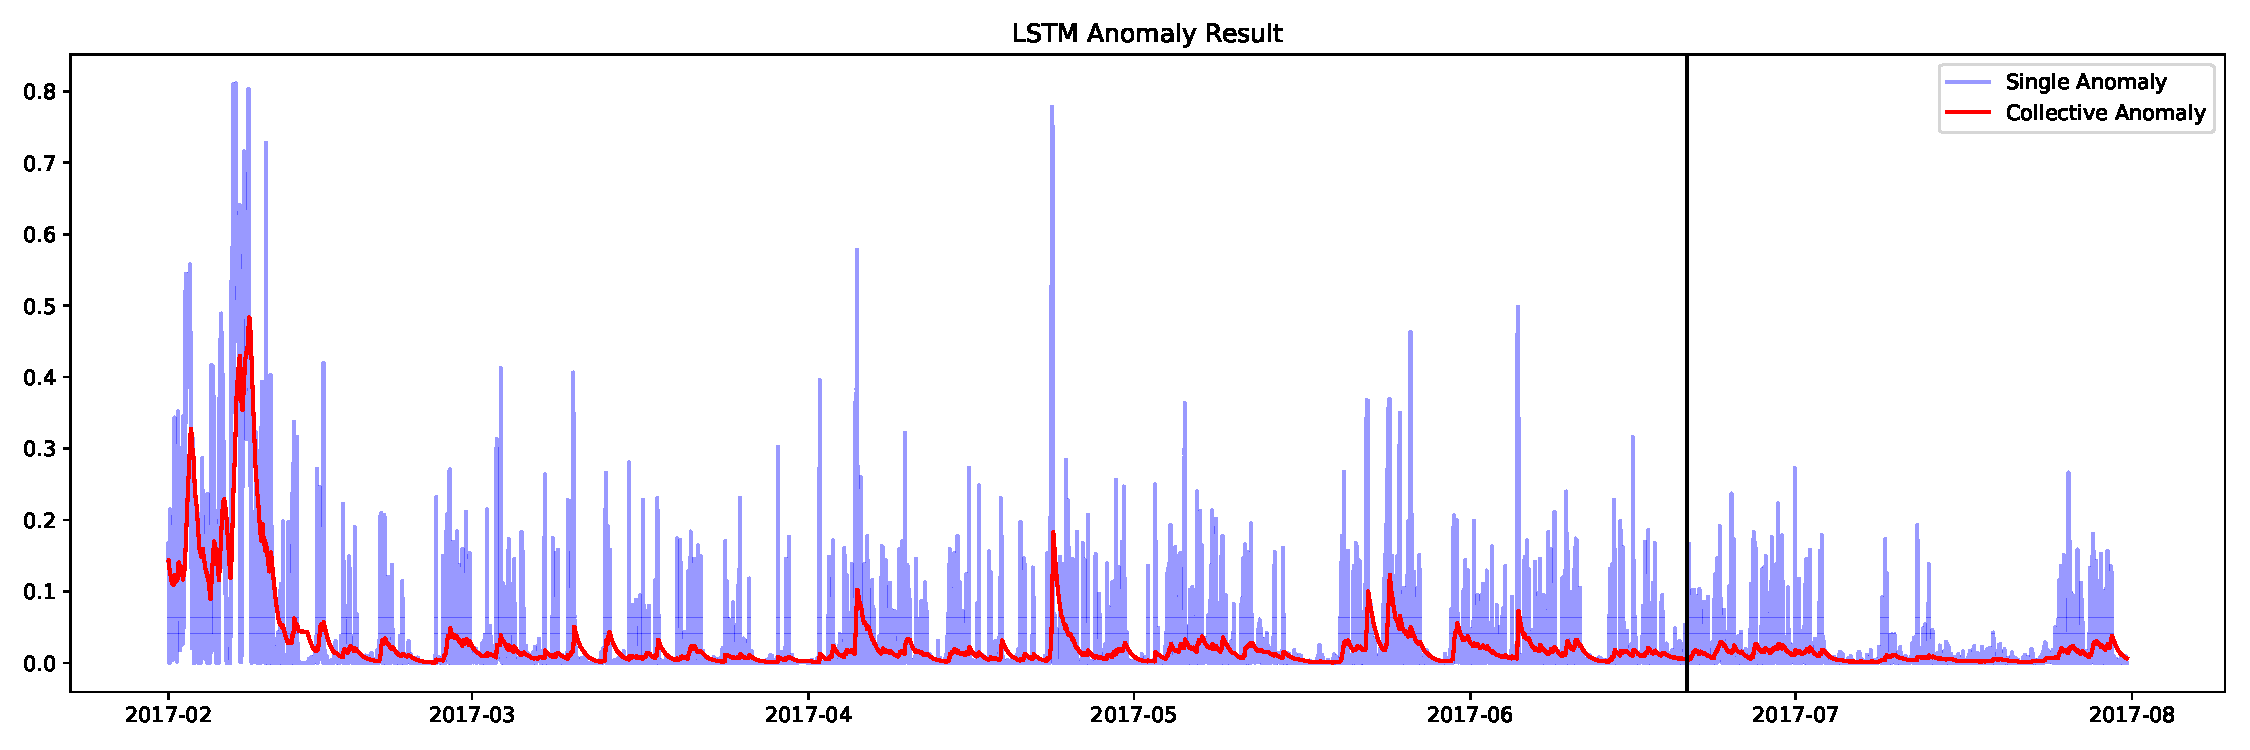
\includegraphics[width=0.48\textwidth]{lstm_anomaly_128_1_tukey.pdf}
       \label{fig:1-lstm-anomaly-figc}
  }
  \vspace{10pt}
  \caption{Anomaly scores of the $1$-layered networks on test data.}
  \label{fig:1-deep_anomalies}
\end{figure}


\begin{figure}
    \centering
  \subfigure[RNN with MSE loss]{
       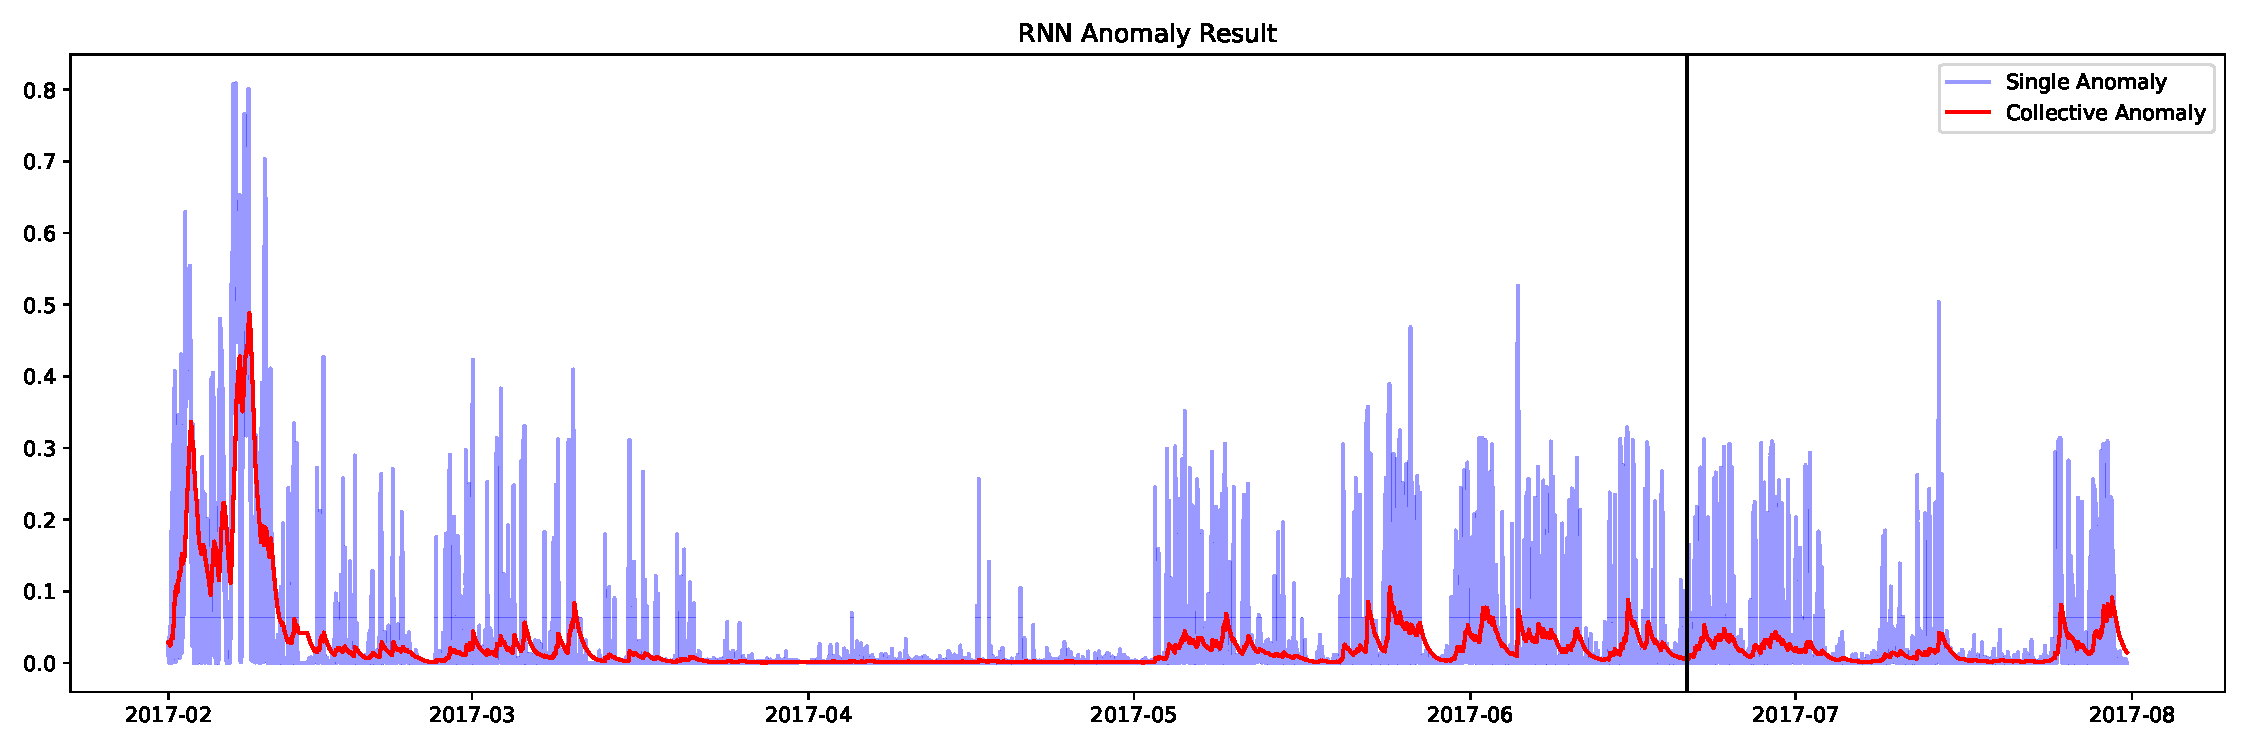
\includegraphics[width=0.48\textwidth]{rnn_anomaly_128_2_MSE.pdf}
       \label{fig:2-rnn-anomaly-figa}
    }%
  \hfill
  \subfigure[LSTM with MSE loss]{
       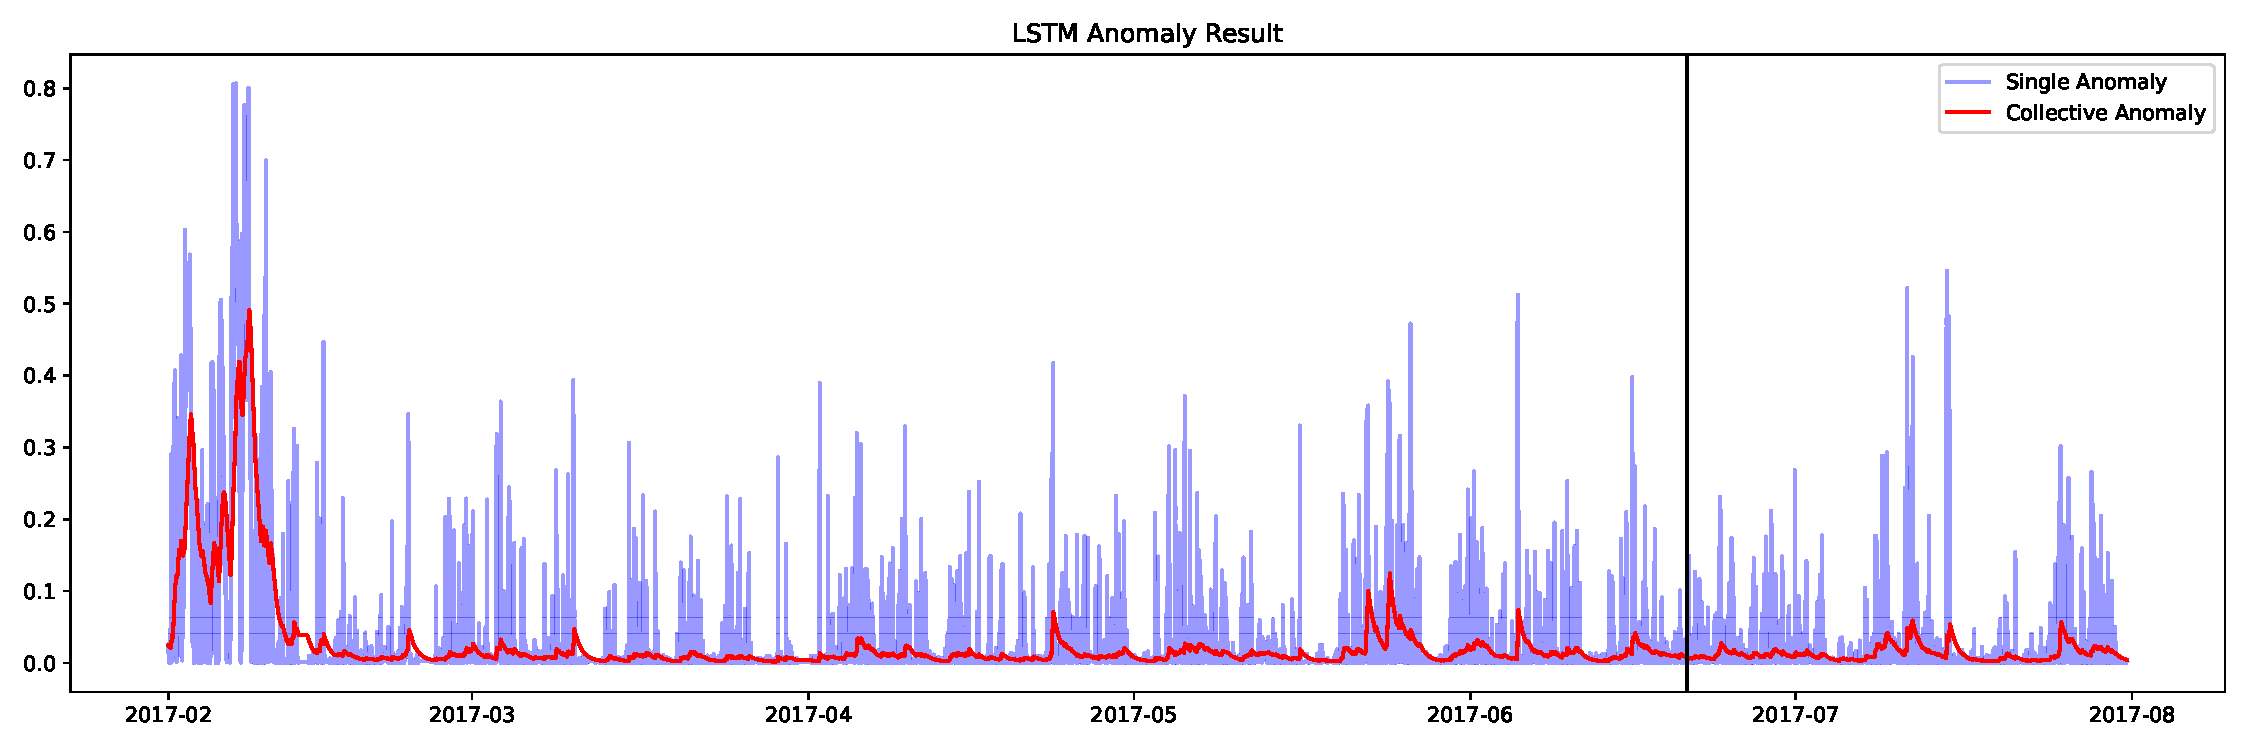
\includegraphics[width=0.48\textwidth]{lstm_anomaly_128_2_MSE.pdf}
       \label{fig:2-lstm-anomaly-figa}
  }
  
  \subfigure[RNN with L1 loss]{
       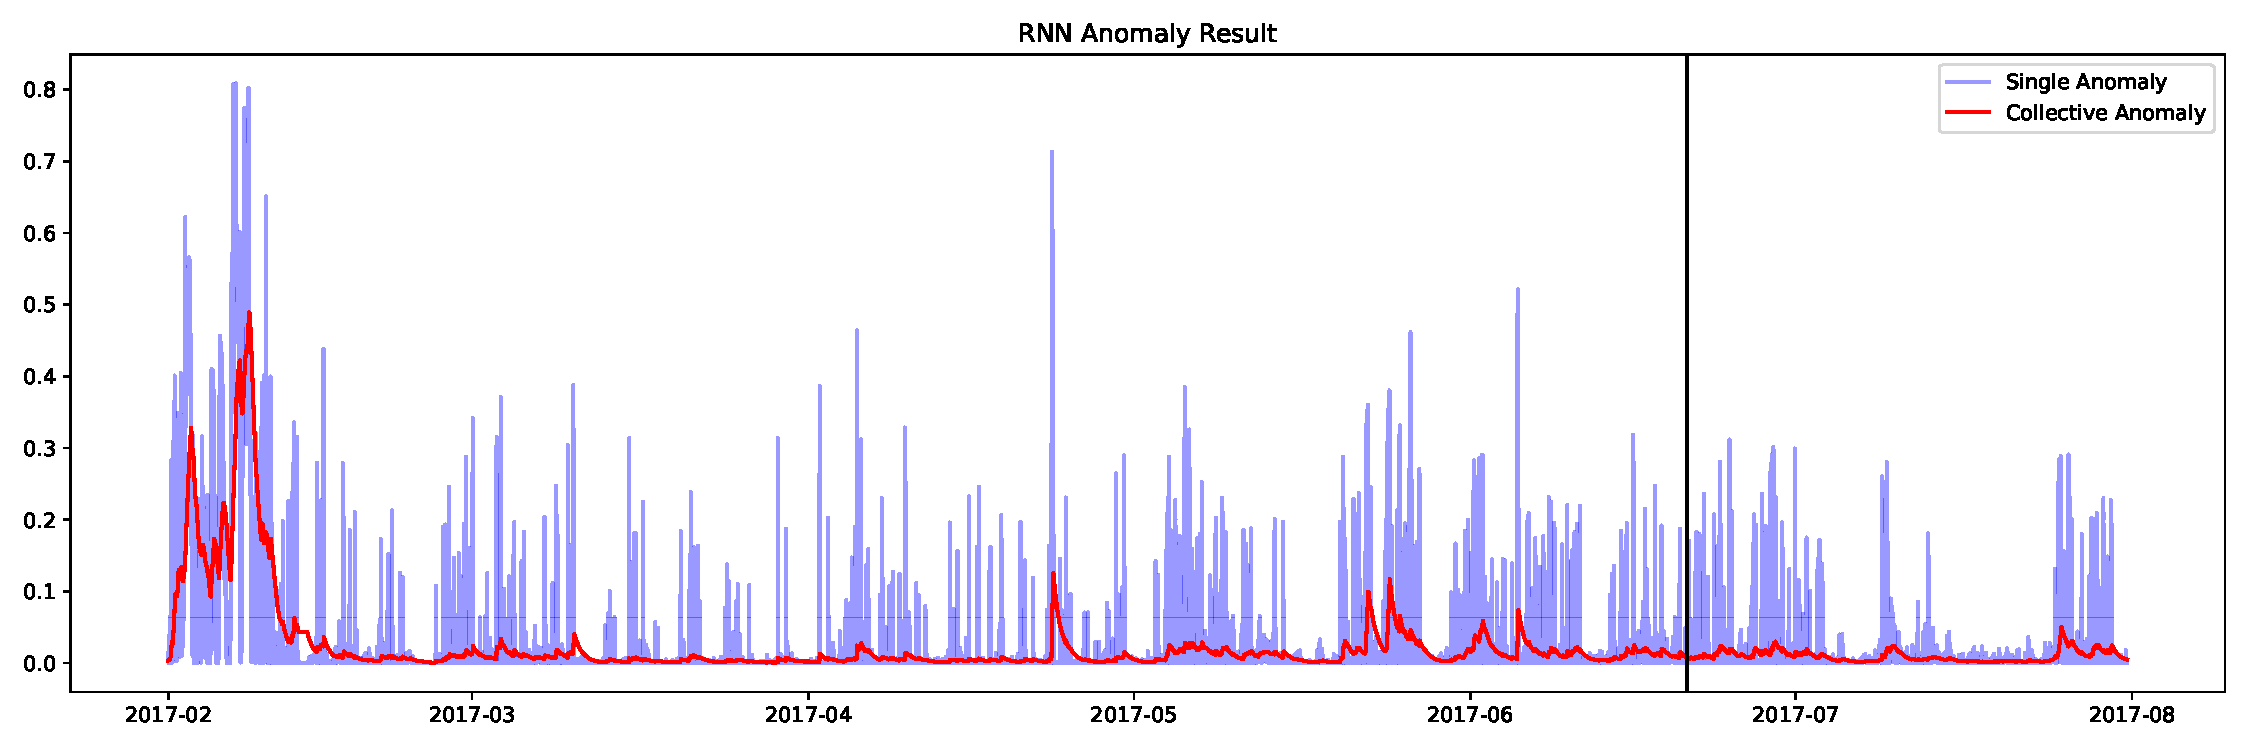
\includegraphics[width=0.48\textwidth]{rnn_anomaly_128_2_L1.pdf}
       \label{fig:2-rnn-anomaly-figb}
  }%
  \hfill
  \subfigure[LSTM with L1 loss]{
       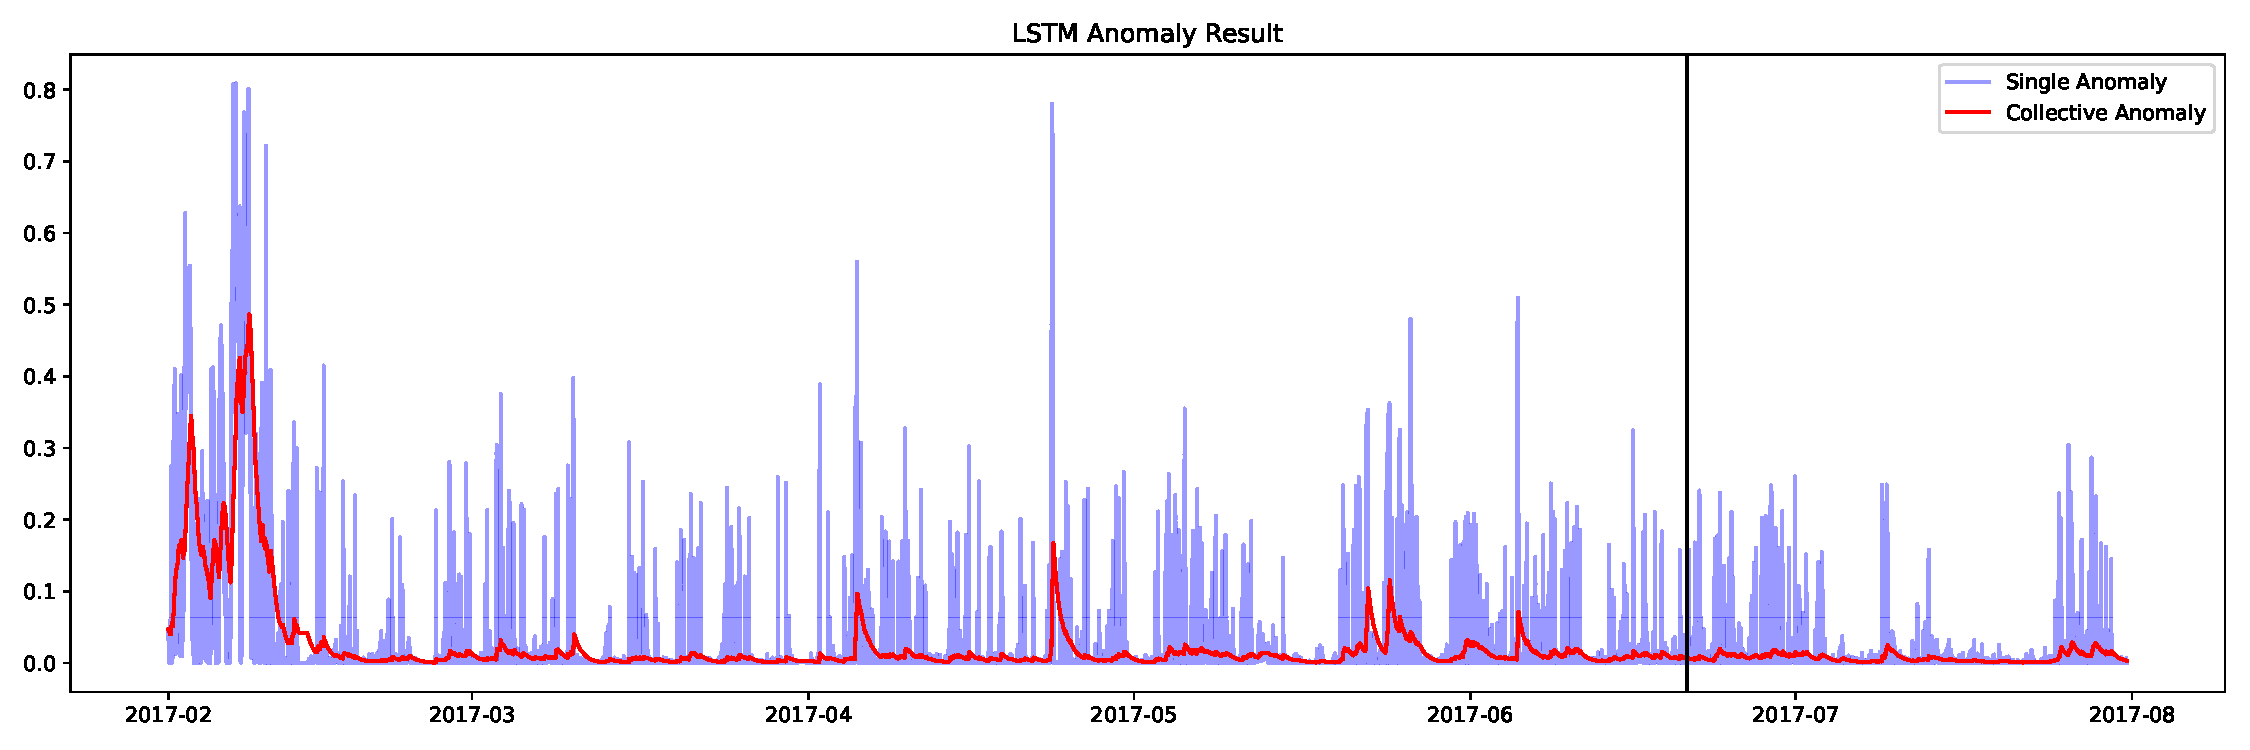
\includegraphics[width=0.48\textwidth]{lstm_anomaly_128_2_L1.pdf}
        \label{fig:2-lstm-anomaly-figb}
  }
  
  \subfigure[RNN with Tukey's biweight loss]{
       %\centering
       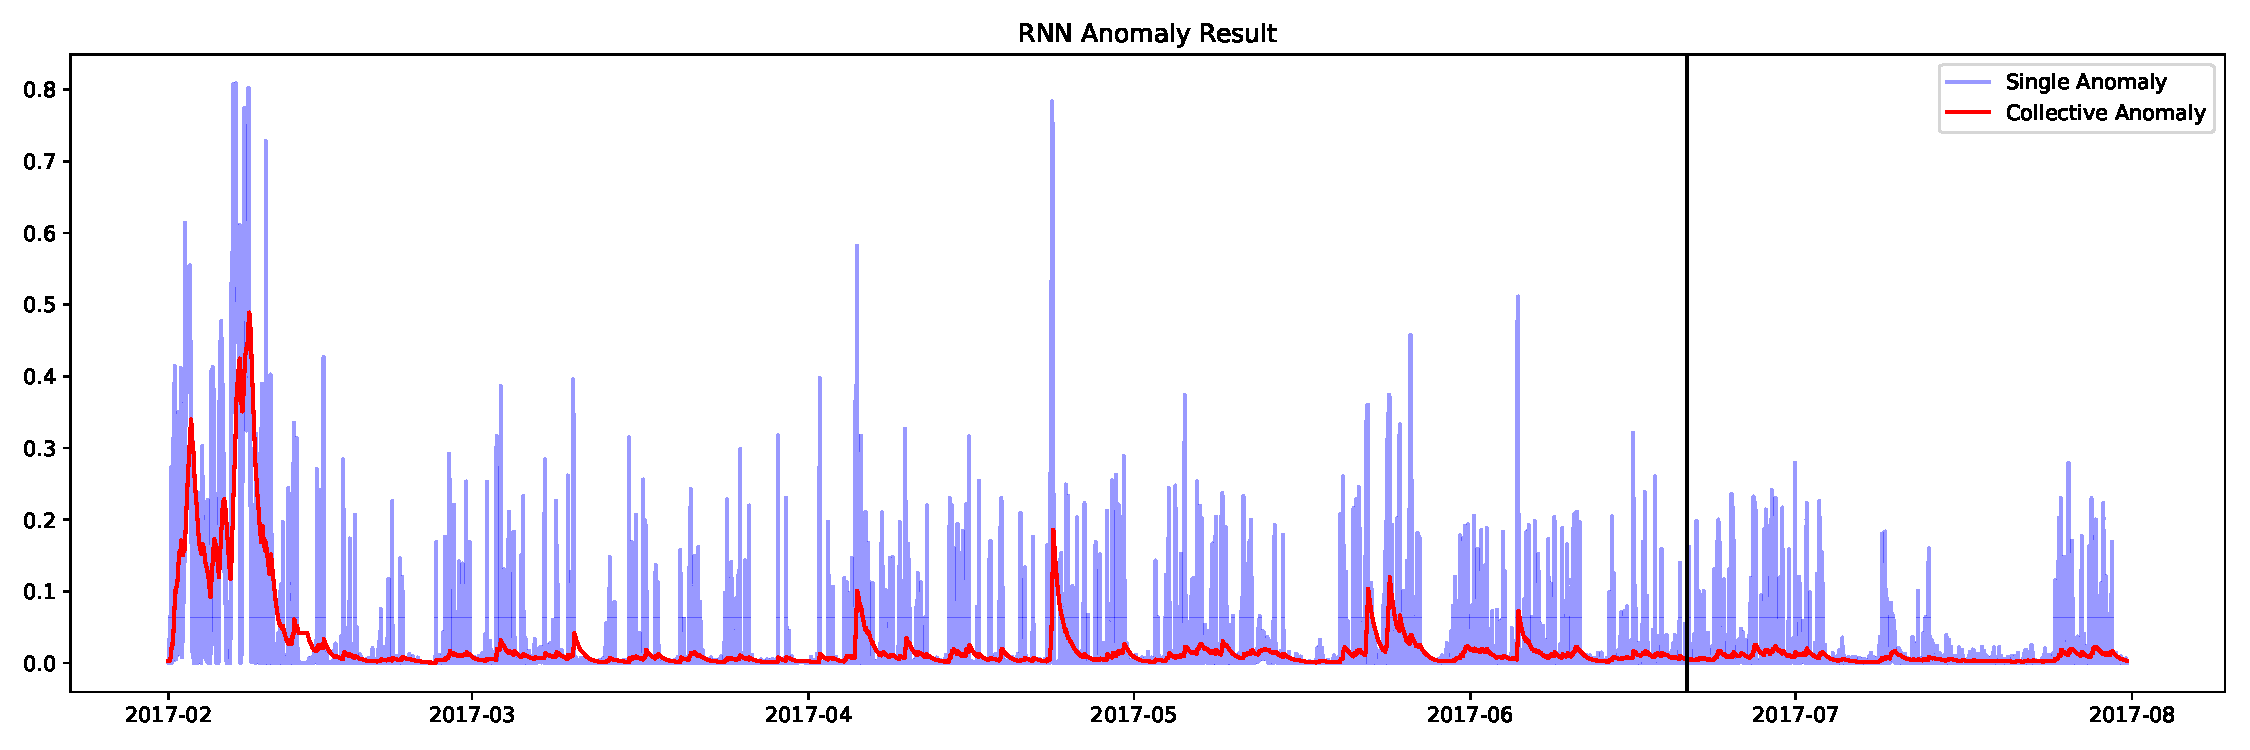
\includegraphics[width=0.48\textwidth]{rnn_anomaly_128_2_tukey.pdf}
        \label{fig:2-rnn-anomaly-figc}
  }%
  \hfill
  \subfigure[LSTM with Tukey's biweight loss]{
       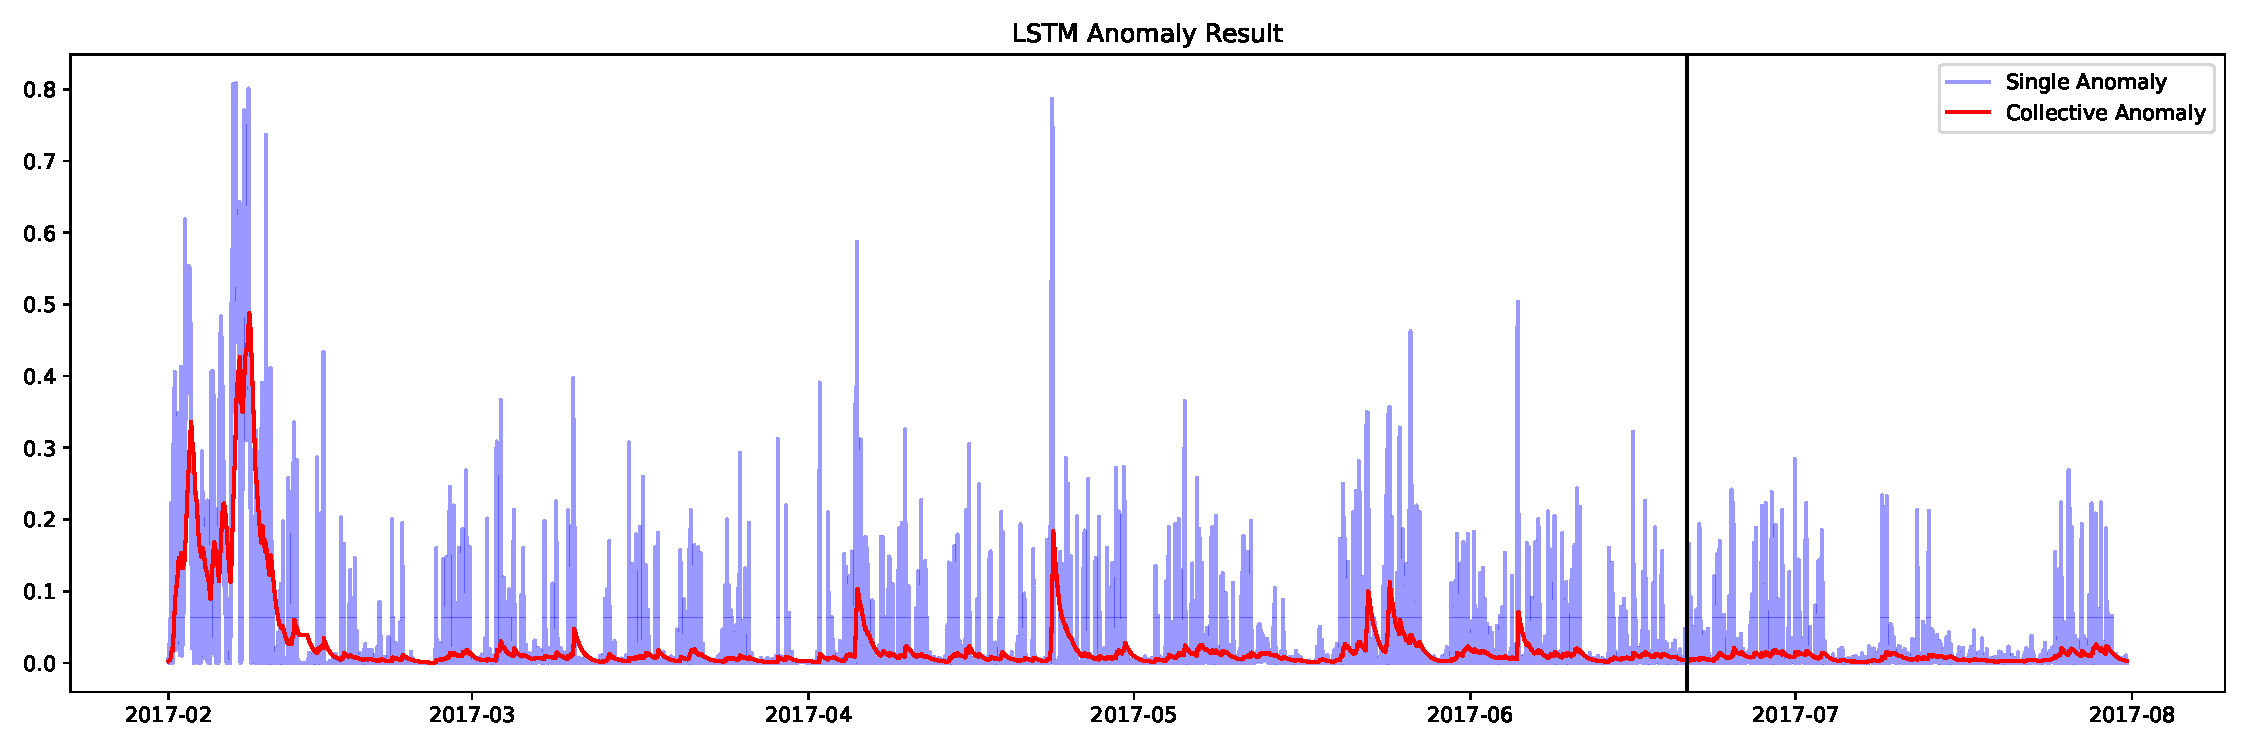
\includegraphics[width=0.48\textwidth]{lstm_anomaly_128_2_tukey.pdf}
       \label{fig:2-lstm-anomaly-figc}
  }
  \vspace{10pt}
  \caption{Anomaly scores of the $2$-layered (stacked) networks on test data.}
  \label{fig:2-deep_anomalies}
\end{figure}

\chapter{CONCLUSION AND FUTURE WORK}
\label{chapter:conclusion-and-future-work}
In this work, we developed some models and algorithms for anomaly detection in time series data.
We conducted our work in two different approaches, which are statistical algorithms and deep learning based sequence models. As a result of this work, we developed two different models that can perform on the same datasets, and that can create a similar anomaly score.

As a statistical approach, we developed a special kind of hidden Markov model which can handle noisy real-world data and can perform anomaly detection task on this data. We assign one additional hidden state, `outlier state' to the latent space to explain noisy, unwanted observations. This is similar to what we did in the GMM. In GMM, we defined Gaussian mixtures, which correspond to latent states of the system, and we represented an additional Gaussian mixture with has high variance, which corresponds to `outlier state' in HMM. However, in GMM, we can track anomalies only from the outlier state. If an observation falls into outlier state, then the model arises an anomaly error. This approach has the following  main drawbacks which we solved with HMM;

\begin{enumerate}
    \item The observations in the outlier state are often not outliers of the system we seek to detect. The observations in this state are mostly composed of errors in the observations.
    \item GMM can not track the state transitions. Therefore, if unexpected observations occur, GMM cannot detect it.
\end{enumerate}

% As deep learning approaches, we propose models which are constructed with RNN and LSTM, respectively. 
The deep learning based models we proposed are constructed with RNN and LSTM.
This part of our study emerged by combining specific parts of two studies \cite{malhotra2015long,bontemps2016collective}. Malhotra et.al. in \cite{malhotra2015long} performed anomaly detection method on cyclic data; on the other hand, Bontemps et.al. in \cite{bontemps2016collective} tried to identify the collective anomalies. 
In the light of these studies, we developed an anomaly detection model which first learns the patterns of the system and then evaluates the new coming observations considering the previous observations. 
This model, similar to HMM, track more complex state transition, and therefore, it can catch the collective anomalies.
We were able to observe the effects of the degree of past dependence on the system.
Since LSTMs are very successful in capturing past links, we are achieving much more successful results with LSTMs when the system has such a dynamic.

As we demonstrated in our experiments, the proposed models are powerful, flexible, and yield good results in an arguably challenging problem. Nonetheless, both models and applications can be further improved in many respects. Possible future research directions are as follows:

\begin{enumerate}
    \item Although our HMM model is successful in detecting anomaly states, it is not equally successful in capturing the change of system over time. Therefore, over time, its performance may decline.
    \item Our LSTM model is successful in capturing collective anomalies but can be sensitive to missing data, which in some cases may adversely affect system performance.
    \item In order to solve the two problems mentioned above, a more complex model can be created including the combination of LSTM and HMM or the particle filter.
    \item Coupled anomaly detection is planned to be developed. Conduction of anomalies in the systems by looking at other parallel systems will improve the analysis and anomaly warnings.
\end{enumerate}


\bibliographystyle{styles/fbe_tez_v11}
\bibliography{references}

\appendix
\chapter{COMPARISON OF THE LOSS FUNCTIONS}
\label{chapter:comparison-of-the-loss-functions}
Neural networks are trained under loss functions. So, for this purpose, we will compare the MSE loss, L1 loss, and Tukey's Biweight loss.

During the analysis, let $r_t = y_t - \hat{y}_t$ is residual for single output and let $\rho(.)$ corresponds to error for given residual. The loss of individual residuals are as follows:

\begin{eqnarray}
\rho(r_t) & = & \frac{1}{2} r_t^2 \label{eq:mse}\\
\rho(r_t) & = & \left|r_t\right| \label{eq:l1}\\
\rho(r_t) & = & \left\{\begin{array}{ll}{\frac{c^{2}}{6}\left[1-\left(1-\left(\frac{r_{i}}{c}\right)^{2}\right)^{3} \right]} & {, \text { if }\left|r_{i}\right| \leq c} \\ {\frac{c^{2}}{6}} & {, \text { if }\left|r_{t}\right|>c}\end{array}\right. \label{eq:tukey}
\end{eqnarray}

Where Equation \ref{eq:mse} corresponds to MSE loss, Equation \ref{eq:l1} refers to L1 loss and Equation \ref{eq:tukey} corresponds to Tukey's biweight loss functions. The results and figures of these losses are shown in the Figure \ref{fig:loss}.

\begin{figure}
    \centering
    \includegraphics[width=0.9\textwidth]{figures/loss.pdf}
    \caption{Comparison of the loss functions}
    \label{fig:loss}
\end{figure}

The gradients of these loss functions are shown in Figure \ref{fig:gradient}.
Mathematically, these gradients are as follows, respectively:

\begin{eqnarray}
\rho^{\prime}(r_t) & = & r_t \label{eq:mse-derivative}\\
\rho^{\prime}(r_t) & = & \left\{\begin{array}{ll}{-1} & {, \text { if }\left|r_{t}\right|<0} \\ {1} & {, \text { if }\left|r_{t}\right|>0}\end{array}\right. \label{eq:l1-derivative}\\
\rho^{\prime}(r_t) & = & \left\{\begin{array}{ll}{r_{i}\left(1-\left(\frac{r_{t}}{c}\right)^{2}\right)^{2}} & {, \text { if }\left|r_{t}\right| \leq c} \\ {0} & {, \text { if }\left|r_{t}\right|>c}\end{array}\right. \label{eq:tukey-derivative}
\end{eqnarray}

\begin{figure}
    \centering
    \includegraphics[width=0.9\textwidth]{figures/gradient.pdf}
    \caption{Comparison of the gradients of loss functions}
    \label{fig:gradient}
\end{figure}

The choice of $c$ of the `Tukey's biweight' loss depends on the `asymptotic efficiency'. Practically it sets to $4.685$, and it provides an asymptotic efficiency $95\%$ that of linear regression for the normal distribution. In the use case, one should calculate the {\it median absolute deviation} (MAD) of the residuals and set the new residuals as follows:

\begin{eqnarray}
    r_{t}^{\mathrm{MAD}} & =& \frac{r_t}{1.4826 \times \mathrm{MAD}_{t}}
\end{eqnarray}

\end{document}